% Load the kaobook class
\documentclass[
	fontsize=10pt, % Base font size
	twoside=true, % Use different layouts for even and odd pages (in particular, if twoside=true, the margin column will be always on the outside)
	%open=any, % If twoside=true, uncomment this to force new chapters to start on any page, not only on right (odd) pages
	secnumdepth=1, % How deep to number headings. Defaults to 1 (sections)
	numbers=noenddot, % Comment to output dots after chapter numbers; most common values are: enddot, noenddot, auto
]{kaobook}

% Choose the language
\usepackage[english]{babel} % Load characters and hyphenation
\usepackage[english=british]{csquotes}	% English quotes

% Load packages for testing
\usepackage{blindtext}


% Packages by Pascal
\let\listofalgorithms\relax
\let\l@algorithm\relax
\usepackage{algorithm}
\usepackage{algpseudocode}
\usepackage{tabularx}
\usepackage{threeparttable}
\usepackage{longtable}
\usepackage{xspace}
\usepackage{enumitem}      % for \setlist — already may be in kaobook, safe to add
\usepackage[edges]{forest}
\usepackage{subcaption}
\usetikzlibrary{trees, positioning, calc}

% Load the bibliography package
\usepackage{kaobiblio}
\addbibresource{thesis.bib} % Bibliography file
\addbibresource{imported_papers/ACU_JAIR/cleaned_references.bib}

% Load mathematical packages for theorems and related environments
\usepackage{kaotheorems}

% Load the package for hyperreferences
\usepackage{kaorefs}

% Load pdfpages for the custom title page
\usepackage{pdfpages}



% ── Custom commands shared across chapters ────────────────────────────────

% ACU survey counters
\newcommand{\numagents}{87\xspace}
\newcommand{\numdatasets}{33\xspace}

% Roman numeral helpers
\newcommand{\uproman}[1]{\uppercase\expandafter{\romannumeral#1}}
\newcommand{\lowroman}[1]{\romannumeral#1\relax}

% Citation aliases — biblatex equivalents
% Natbib-style \citet[pre][post]{key} and \citep[pre][post]{key}
\providecommand{\citet}{}
\providecommand{\citep}{}
\RenewDocumentCommand{\citet}{o o m}{%
    \IfNoValueTF{#1}{\textcite{#3}}{%
        \IfNoValueTF{#2}{\textcite[#1]{#3}}{\textcite[#1][#2]{#3}}}%
}
\RenewDocumentCommand{\citep}{o o m}{%
    \IfNoValueTF{#1}{\parencite{#3}}{%
        \IfNoValueTF{#2}{\parencite[#1]{#3}}{\parencite[#1][#2]{#3}}}%
}

% \citepeg{key} → (e.g., Author 20XX)
\NewDocumentCommand{\citepeg}{m}{%
    \parencite[e.g.,][]{#1}%
}

% ACM template no-ops for imported papers
\providecommand{\Description}[2][]{}
\providecommand{\numpapers}{87\xspace}

% cleveref name overrides — place AFTER kaorefs loads cleveref
\crefname{figure}{Figure}{Figures}
\Crefname{figure}{Figure}{Figures}
\crefname{section}{Section}{Sections}
\Crefname{section}{Section}{Sections}
\crefname{equation}{Eq.}{Eqs.}
\Crefname{equation}{Eq.}{Eqs.}
\crefname{appendix}{Appendix}{Appendix}
\Crefname{appendix}{Appendix}{Appendix}
\crefname{table}{Table}{Table}
\Crefname{table}{Table}{Table}




\graphicspath{{images/}{./}{figures/}{imported_papers/ACU_JAIR/figures/}{imported_papers/ACU_JAIR/}} % Paths where images are looked for

\makeindex[columns=3, title=Alphabetical Index, intoc] % Make LaTeX produce the files required to compile the index

% Load custom thesis styles (colors, fonts, etc.)
% -------------------------------------------------------------
% thesis_style.tex
% This file defines custom style updates for the PhD thesis,
% including colors and fonts.
% -------------------------------------------------------------

% 1. Define custom colors for the document
% You can change these RGB values to match your university's branding
\definecolor{ThesisDarkRed}{RGB}{140, 0, 0}
\definecolor{ThesisAccentRed}{RGB}{210, 0, 0}
\definecolor{ThesisGray}{RGB}{100, 100, 100}

% 2. Update font formatting for headings using KOMA-Script commands
% This applies the dark blue color to chapters, sections, etc.
\addtokomafont{chapter}{\color{ThesisDarkRed}}
\addtokomafont{section}{\color{ThesisDarkRed}}
\addtokomafont{subsection}{\color{ThesisAccentRed}}
\addtokomafont{subsubsection}{\color{ThesisAccentRed}}
\addtokomafont{paragraph}{\color{ThesisAccentRed}}
\addtokomafont{captionlabel}{\color{ThesisDarkRed}\bfseries}
\addtokomafont{pagenumber}{\color{ThesisGray}}

% 3. Update hyperlink colors
% Here we apply the custom colors to links, citations, and URLs
\hypersetup{
    colorlinks=true,
    linkcolor=black,
    filecolor=black,
    urlcolor=ThesisDarkRed,
    citecolor=ThesisDarkRed,
}

% 4. Enable chapter formatting
% kaobook supports different chapter styles (e.g. kao, plain)
\setchapterstyle{kao}

% 5. Cross-referencing helpers using cleveref
% This ensures consistent formatting (e.g., "Figure" vs "Fig." etc.) across the document.
% By default kaobook uses noabbrev for cleveref. If you prefer abbreviations
% (so \cref outputs Fig. instead of Figure), uncomment the next lines:
% \crefname{figure}{Fig.}{Figs.}
% \Crefname{figure}{Fig.}{Figs.}
% \crefname{equation}{Eq.}{Eqs.}
% \Crefname{equation}{Eq.}{Eqs.}
% \crefname{table}{Tab.}{Tabs.}
% \Crefname{table}{Tab.}{Tabs.}
% \crefname{section}{Sec.}{Secs.}
% \Crefname{section}{Sec.}{Secs.}

% Standardized helper macros bridging to \cref
\newcommand{\figref}[1]{\cref{#1}}
\newcommand{\tabref}[1]{\cref{#1}}
\newcommand{\secref}[1]{\cref{#1}}
\newcommand{\chapref}[1]{\cref{#1}}
\newcommand{\eqnref}[1]{\cref{#1}}
\newcommand{\appref}[1]{\cref{#1}}


\begin{document}

\frontmatter % Denotes the start of the pre-document content, uses roman numerals

%----------------------------------------------------------------------------------------
%	OUTPUT TITLE PAGE
%----------------------------------------------------------------------------------------

% Include the custom title page
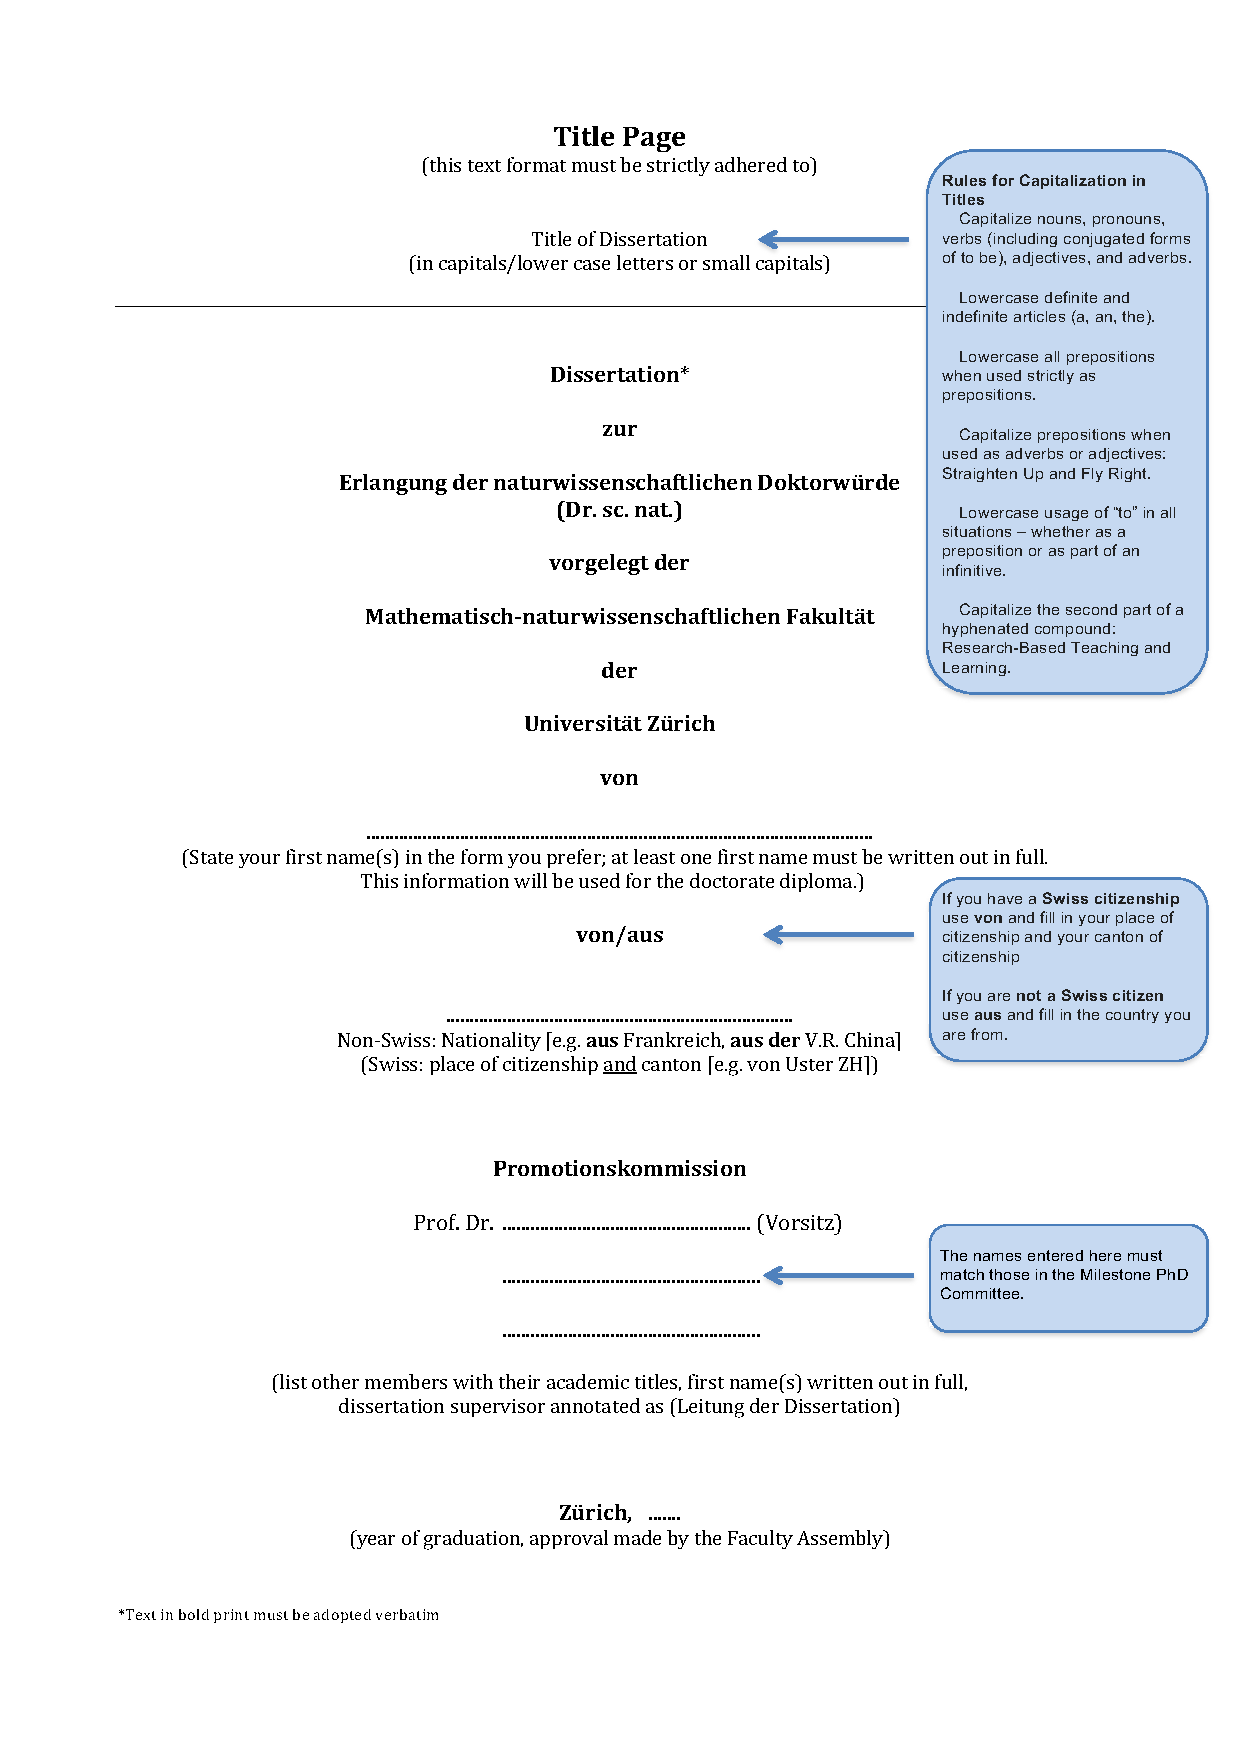
\includepdf[pages=-]{figures/Titelblatt_E_POV2011.pdf}

%%%%%%%%%%%%%%%%%%%%%%%%%%%%%%%%%%%%%%%%%%%%%%%%%%%%%%%%%%%%%%%%%%%%%%%%%%%%%%%%
%\titlehead{Doctoral Dissertation}

\subject{Doctoral Dissertation}
\title[Bridging the Agentic Gap]{
    Bridging the Agentic Gap
}
\subtitle{Dual Paradigms in Structured Representations and Deep Generative World Models}

\author[Pascal Sager]{Pascal Sager}
\date{December 1, 2026}
\publishers{University of Zurich}

\maketitle

%----------------------------------------------------------------------------------------
%	ABSTRACT
%----------------------------------------------------------------------------------------

\chapter*{Abstract}
\addcontentsline{toc}{chapter}{Abstract}
%
%
The past decade of deep learning has produced systems of impressive capability, 
yet their deployment in demanding real-world settings consistently exposes a 
recurring cluster of failures: brittleness to distributional shift, inability 
to compose learned concepts in novel ways, and error accumulation that renders 
long-horizon planning unreliable. This thesis argues that these failures are 
not incidental engineering shortcomings but structural consequences of how 
current architectures represent knowledge. We propose a research direction that 
moves from diagnosing these failures, through mitigating them with principled 
constraints, toward a paradigm shift grounded in neuro-inspired computation.

We begin with a comprehensive survey and taxonomy of agents for computer use 
(ACUs), systems that automate complex tasks on digital devices given 
natural-language instruction. Covering 87 research papers and 33 benchmark 
datasets, we identify six persistent research gaps, including insufficient 
generalisation, limited planning, and a disconnect between laboratory evaluation 
and real-world deployment. We argue that these gaps are symptomatic of 
structural limitations in the underlying learning paradigm rather than a matter 
of scale alone. Two supporting studies corroborate this diagnosis from 
independent directions. A benchmark of efficient large language models shows 
that the compression methods currently needed to make these models accessible 
systematically degrade the reasoning capabilities they are meant to preserve. 
A compositional visual reasoning framework further demonstrates that 
state-of-the-art architectures, including those with strong inductive biases 
for compositionality, consistently fail to generalise to novel rule combinations.

To understand the origin of these failures, we develop a mathematical framework 
for analysing the representational geometry of self-attention matrices. We prove 
that the choice of training objective, bidirectional versus autoregressive, 
dictates a precise structural signature in the learned weight matrices: symmetry 
in the former, directionality and column dominance in the latter. These results 
are validated across ModernBERT, GPT, LLaMA3, and Mistral on text, vision, and 
audio modalities. They establish that the geometry of learned representations is 
a mathematical consequence of the training objective. Current architectures do 
not discover structure in the world; they embed the statistical structure of 
their loss function.

Given this diagnosis, we investigate whether imposing hard, mathematically 
grounded constraints on deep learning systems can correct specific failure modes. 
We introduce \textit{Koopman-JEPA}, a self-supervised world model that lifts 
complex visual observations into a latent space governed by globally linear 
dynamics. In standard nonlinear world models, approximation errors compound 
exponentially across rollout steps via the Lipschitz constant of the composed 
functions. By replacing these nonlinear rollouts with matrix multiplications 
over a stable linear operator, error accumulation is bounded to grow linearly 
with horizon. Three variants with progressively stronger spectral constraints 
on the transition matrix culminate in a Cayley parameterisation that 
architecturally enforces strict stability and satisfies the stabilisability 
precondition of discrete-time linear quadratic regulation. Koopman variants 
reduce long-horizon prediction error by up to 99\% on action-free tasks and 
91\% on action-conditioned tasks at a ten-step horizon, while improving sample 
efficiency by approximately sixteen-fold when only ten percent of training data 
is available. Two complementary studies show that the constraint principle 
generalises across domains. Encoding tissue-specific Hounsfield unit ranges as 
binary input masks compensates for data scarcity in clinical CT segmentation, 
and a hybrid retrieval architecture that grounds predictions via external 
structured knowledge achieves first place on the CLEF CheckThat! 2025 
development leaderboard without any external training data.

Finally, we ask whether constraint engineering alone is sufficient or whether 
the representational substrate must itself change. We introduce the 
\textit{Cooperative Network Architecture} (CNA), which replaces distributed 
activation patterns with dynamically assembled, recurrently connected networks 
of neurons called \textit{nets}, built from overlapping fragments learned 
without supervision from regularities in sensory input. Because nets are 
composable by construction, CNA exhibits figure completion, noise resilience, 
and generalisation to out-of-distribution patterns without retraining. These 
properties emerge from the representational principle of the architecture rather 
than from loss engineering.

Together, these contributions trace a path from empirical diagnosis through 
principled mitigation to architectural reconception. We conclude that 
constraint-based approaches offer the most immediate practical gains, but that 
achieving robust and composable intelligence ultimately requires representational 
structures that embed invariance and compositionality by design, a direction in 
which neuro-inspired computation remains the most principled guide.


\chapter*{Zusammenfassung}
\addcontentsline{toc}{chapter}{Zusammenfassung}
\input{sections/0-2_abstract_de}

%----------------------------------------------------------------------------------------
%	PREFACE
%----------------------------------------------------------------------------------------

\chapter*{Preface}

The journey culminating in this thesis, *Bridging the Agentic Gap*, has been anything but a straight line. If my publication record leading up to this point appears somewhat fragmented, it is a direct reflection of my genuine, unbridled excitement for the field of Artificial Intelligence. I have always been drawn to diverse ideas and collaborations, and while this led me down varied research paths, at the given time and context, pursuing every single one of those threads made perfect sense. Ultimately, it was this wide-ranging curiosity that allowed me to synthesize the dual paradigms presented in this work: the biologically-inspired structural approach of neuroscience and the scalable realm of deep generative world models.

This journey truly began when my original plan to pursue a full-time Master's degree was wonderfully derailed. Prof. Dr. Thilo Stadelmann offered me the opportunity to study part-time while working in his research lab. That decision changed everything. I stayed on through my subsequent studies and into this PhD, always feeling incredibly fortunate for the immense freedom and decision-making power I was given to explore the topics I was most passionate about. Thilo, thank you for your mentorship, for sponsoring my initial fellowship, and for the countless highlights at the ZHAW Centre for Artificial Intelligence. It has been a pleasure being a part of this journey, from the centre's founding to its growth into seven research groups. 

I am equally indebted to the head of my committee, Prof. Dr. Benjamin Grewe, who so warmly welcomed me into his lab. The opportunity to work at the intersection of neuroscience and AI under your guidance was instrumental in shaping the foundational concepts of this thesis. I would also like to express my sincere gratitude to Prof. Dr. Giacomo Indiveri for serving on my committee, as well as to Dr. Jan Milan Deriu, Dr. Jorge Peña Querlata, and Prof. Dr. Christoph von der Malsburg, all of whom provided vital support, insights, and encouragement during different phases of my research.

My research was also made possible through the generous support of the DIZH (Digitalization Initiative of the Zurich Higher Education Institutions), and I am deeply grateful to the Canton of Zurich for awarding me the fellowship that funded the latter stages of this work.

Finally, the most profound thanks belong to my family. Over the course of this PhD, our family beautifully grew from three to five. To my wonderful wife, Dona Belle: thank you for your endless patience, your unwavering support, and for keeping everything together while I was lost in research. To my oldest son, Leeroy, and my daughters, Reyna and Elody: you are my greatest achievements. Thank you for reminding me every day of the real world outside of deep learning models. 


%----------------------------------------------------------------------------------------
%	TABLE OF CONTENTS & LIST OF FIGURES/TABLES
%----------------------------------------------------------------------------------------

\begingroup % Local scope for the following commands

% Define the style for the TOC, LOF, and LOT
\setlength{\textheight}{230\vscale} % Manually adjust the height of the ToC pages

% Turn on compatibility mode for the etoc package
\etocstandarddisplaystyle % "toc display" as if etoc was not loaded
\etocstandardlines % "toc lines as if etoc was not loaded

\tableofcontents % Output the table of contents

\listoffigures % Output the list of figures

\let\cleardoublepage\bigskip
\let\clearpage\bigskip

\listoftables % Output the list of tables

\endgroup

%----------------------------------------------------------------------------------------
%	MAIN BODY
%----------------------------------------------------------------------------------------

\mainmatter % Denotes the start of the main document content, resets page numbering and uses arabic numbers
\setchapterstyle{kao} % Choose the default chapter heading style



%----------------------------------------------------------------------------------------
%	PART I: THE FOUNDATION
%----------------------------------------------------------------------------------------

\pagelayout{wide}
\addpart{The Foundation}
\pagelayout{margin}

\chapter{Introduction}\label{chap:introduction}
\margintoc
% ─────────────────────────────────────────────────────────────────────────────
\section{The Gap Between Competence and Understanding}
\label{sec:intro_gap}
% ─────────────────────────────────────────────────────────────────────────────

The past decade of machine learning research has been defined by a striking
asymmetry. Progress on benchmarks has been rapid and measurable. Progress on
the underlying question of what learned representations actually encode has
been slow and contested. The two trajectories have now diverged to a degree
that demands explanation.

Contemporary deep learning systems achieve results that would have seemed
implausible a decade ago. Large language models pass professional licensing
examinations, synthesise code from natural-language specifications, and
produce coherent text across domains that require substantial world
knowledge~\cite{brown_gpt3, wei_emergent}. Vision systems trained on
internet-scale data match or exceed human performance on curated image
classification benchmarks~\cite{dosovitskiy_vit, zhai_scaling}. Reinforcement
learning agents master games of enormous strategic depth, from Go to
StarCraft~\cite{silver_alphago, vinyals_starcraft}. By the standard measures
of the field, progress has been exceptional.

Yet when these same systems are placed outside the conditions under which they
were evaluated, a different picture emerges. An agent that reliably completes
multi-step tasks on familiar software interfaces fails when the interface
changes, when the task sequence is novel, or when an unexpected state requires
a response not present in its training distribution~\cite{acu_survey}. A
language model that solves competition-level mathematics cannot reliably apply
a simple spatial rule to a grid of objects it has not seen
before~\cite{cogitao}. A world model that accurately predicts one step ahead
diverges catastrophically over a ten-step horizon, accumulating errors that
render its predictions useless for planning~\cite{koopman_jepa}. These are not
isolated failures attributable to insufficient data or model capacity. They
form a pattern.

The pattern is this: current deep learning systems exhibit high competence
within the statistical regime of their training distribution and brittle
behaviour outside it. They are sensitive to surface features in ways that
suggest their internal representations do not encode the structural properties
of their environment. They fail at tasks that require composing learned
concepts in configurations not encountered during training. And they degrade
under distribution shift in ways that are disproportionate to the magnitude
of the shift. These observations are not new, and individual instances of them
have been documented extensively in the
literature~\cite{geirhos_shortcut, lake_generalization, marcus_deep_learning}.
What has been lacking is a unifying account of why they occur and what, if
anything, can be done about them.

This thesis provides such an account. We argue that the failures listed above
are not incidental consequences of imperfect training or insufficient scale.
They are structural consequences of what gradient-based optimisation on a
fixed objective actually produces: representations whose geometry is
determined by the statistical structure of the training signal rather than
by the causal structure of the world. This claim is not merely
programmatic. In Chapter~\ref{chap:selfattention} we establish it
mathematically for the case of self-attention, the representational mechanism
at the core of modern Transformer architectures, and validate it empirically
across multiple model families and input modalities. From this diagnosis,
two distinct lines of response follow, each explored in depth in the
chapters that follow.


% ─────────────────────────────────────────────────────────────────────────────
\section{The Standard Explanation and Why It Is Insufficient}
\label{sec:intro_scaling}
% ─────────────────────────────────────────────────────────────────────────────

The dominant response to the observed failure modes has been to appeal to
scale. The empirical scaling laws of~\cite{kaplan_scaling, hoffmann_chinchilla}
show that model performance on standard benchmarks improves predictably with
increases in parameter count, dataset size, and compute budget. Under this
view, the failures described above are temporary artefacts of systems that are
not yet large enough: with sufficient scale, generalisation will follow.

We take this argument seriously. The empirical evidence for scaling is
substantial, and dismissing it would be intellectually dishonest. The question
is not whether scale produces improvements, but whether it addresses the
specific class of failures that motivates this thesis. We argue that it does
not, and we present two bodies of evidence in support of this claim.

The first concerns the relationship between model capacity and practical
usability. The compression methods currently required to deploy large models in
resource-constrained settings, including quantisation and low-rank
adaptation~\cite{dettmers_qlora, hu_lora}, do not merely reduce a model's
memory footprint. They degrade its reasoning capabilities in ways that are
disproportionate to the degree of compression applied~\cite{private_llm}. In a
systematic benchmark covering seven methods across two major families of
efficient inference technique, we find that quantised models exhibit
qualitative deterioration in text quality and structured reasoning that is
detectable both by automated metrics and by human evaluators, even at
quantisation levels that are routinely described as lossless in the
literature~\cite{private_llm}. This finding matters for the scaling argument
because it reveals that the capabilities produced by large-scale training are
not robustly encoded: they are sensitive to the precise arithmetic used to
represent the weights. A representation that encodes genuine structural
knowledge of its domain should not be so fragile.

The second body of evidence concerns compositional generalisation. If the
failures observed in deployed systems were primarily a scale problem, one would
expect them to diminish as model capacity increases, and to be
particularly severe in architectures that lack specific structural inductive
biases. We find the opposite. Using the COGITAO framework~\cite{cogitao},
a controlled evaluation environment for compositional and systematic
generalisation in object-centric visual reasoning, we test architectures that
incorporate precisely the inductive biases that compositionality is thought to
require: diffusion-based Transformers and recurrent architectures with
adaptive computation time. Despite strong in-domain performance, these models
fail systematically when task rules are composed in configurations not seen
during training~\cite{cogitao}. The failure is not ameliorated by the
inductive biases; it appears to be a deeper property of how gradient-based
learning encodes multi-step relational structure.

Taken together, these findings suggest that the failures are not primarily
a quantitative shortfall in scale or a qualitative shortfall in architecture
design. They point instead to something more fundamental: a mismatch between
what gradient-based optimisation on a fixed objective produces and what is
required for reliable performance on tasks that demand structured understanding.


% ─────────────────────────────────────────────────────────────────────────────
\section{A Structural Diagnosis: Training Objectives Shape Representations}
\label{sec:intro_diagnosis}
% ─────────────────────────────────────────────────────────────────────────────

To understand the source of these failures, it is necessary to examine what
backpropagation-trained systems actually learn. The standard account describes
learning as function approximation: given a dataset and a loss function, gradient
descent finds parameters that minimise the loss, and the resulting function
generalises to new inputs to the extent that those inputs are drawn from the
same distribution as the training data. This account is accurate as far as it
goes. The question it leaves open is what structure the learned function has
beyond its loss value, and whether that structure is appropriate for the tasks
to which the system will be applied.

We address this question directly in Chapter~\ref{chap:selfattention}, where we
develop a mathematical framework for analysing the internal structure of
self-attention matrices in trained Transformer models. Self-attention is not
merely a component of modern architectures; it is the primary mechanism by
which these models organise and retrieve information, and understanding its
representational geometry is essential for understanding what these models
know and how they know it.

Our central finding is the following. The structural properties of learned
self-attention weight matrices are determined by the training objective, not
by the content of the training data. Bidirectional training objectives, of the
kind used in encoder models such as BERT and ModernBERT, induce symmetry in the
self-attention weight matrices. Autoregressive training objectives, of the kind
used in decoder models such as GPT, LLaMA, and Mistral, induce directionality
and column dominance. These structural signatures are not noise; they are
mathematically derivable from the gradient flow induced by each objective, and
they are empirically consistent across model families and across input
modalities including text, vision, and audio~\cite{selfattention_structures}.

The implication of this result for the question of generalisation is direct.
If the geometry of a model's representations is determined by the structure
of its training objective, then the representations encode the statistical
patterns that the objective is sensitive to, not the causal or structural
properties of the domain from which the training data was drawn. A model
trained with a next-token prediction objective does not, as a consequence of
that training, learn that objects in the world have stable identities, that
causes precede effects, or that rules compose in a specific algebraic
structure. It learns to predict the next token. The representations it develops
are optimised for that task and are well-calibrated within the statistical
regime where that task is well-defined. Outside that regime, they carry no
guarantees.

This diagnosis is not a claim that Transformer models are useless or that they
learn nothing of value. They clearly do learn a great deal. The claim is more
specific: the structure of what they learn is shaped by the objective, and
the failure modes observed empirically are predictable consequences of this
shaping. Compositional generalisation fails because the training objective does
not make the model sensitive to compositional structure; it makes the model
sensitive to co-occurrence statistics. Long-horizon planning fails because no
standard training objective rewards the model for maintaining internally
consistent predictions over extended sequences of interactions. Distributional
robustness fails because the representations are calibrated to the training
distribution, not to the underlying generative process that produced it.

This diagnosis raises a precise research question: given that these failures
are structural properties of what gradient-based learning on standard objectives
produces, what can be done? We pursue two distinct lines of response in this
thesis, which we introduce in the following section.


% ─────────────────────────────────────────────────────────────────────────────
\section{Two Lines of Response}
\label{sec:intro_responses}
% ─────────────────────────────────────────────────────────────────────────────

The diagnosis of Section~\ref{sec:intro_diagnosis} admits two logically
distinct responses. The first accepts the basic framework of gradient-based
learning on fixed objectives and asks whether hard mathematical constraints,
imposed architecturally or through domain knowledge, can correct specific
failure modes before they manifest. The second asks whether the representational
substrate must itself change: whether the class of architectures that
gradient-based learning is applied to needs to be fundamentally reconceived.
We pursue both, and we are explicit about what each can and cannot achieve.

\subsection{Hard Constraints as Structural Corrections}
\label{subsec:intro_constraints}

If a failure mode can be identified precisely enough to be formalised, it can
often be corrected by imposing a constraint that prevents it. This is the
principle underlying the first line of response, and we instantiate it
across three domains in Chapters~\ref{chap:koopman}
and~\ref{chap:constraints}.

The most precise instance concerns multi-step prediction in learned world
models. In any nonlinear world model, approximation errors compound across
rollout steps: each step applies a function with some Lipschitz constant
greater than one, and errors at each step are amplified by that constant in
subsequent steps, producing exponential divergence over long
horizons~\cite{koopman_jepa}. This failure is not a consequence of
insufficient model capacity or imperfect training. It is a mathematical
property of nonlinear function composition. It cannot be corrected by scaling
or by improved optimisation, because it is structural.

We address this failure in Chapter~\ref{chap:koopman} by introducing
Koopman-JEPA, a self-supervised world model that lifts complex visual
observations into a latent space where the dynamics of the environment are
represented by a globally linear operator. In this lifted space, multi-step
prediction reduces to iterated matrix multiplication, and error accumulation
is bounded to grow linearly with horizon rather than exponentially. We develop
three variants with progressively stronger spectral constraints on the
transition matrix, culminating in a Cayley parameterisation that
architecturally enforces strict stability and satisfies the stabilisability
precondition of discrete-time linear quadratic regulation. The empirical
results are correspondingly precise: Koopman variants reduce long-horizon
prediction error by up to 99\% on action-free tasks and 91\% on
action-conditioned tasks at a ten-step horizon, compared to a baseline that
diverges catastrophically at the same horizon~\cite{koopman_jepa}.

The constraint principle is not limited to dynamics. In Chapter~\ref{chap:constraints},
we examine two further cases where structural knowledge, encoded as a hard
constraint, compensates for what unconstrained gradient-based learning fails
to recover. In the domain of clinical image segmentation, encoding
tissue-specific Hounsfield unit ranges as binary input masks, a constraint
derived directly from the biophysics of X-ray attenuation documented in the
medical literature, improves segmentation accuracy by up to 5\% on
intramuscular adipose tissue and enables a model trained on 50\% of the
available data to match the performance of one trained on the
full dataset~\cite{hu_ranges}. In the domain of information retrieval, a
hybrid pipeline that combines lexical precision, dense semantic retrieval, and
large-language-model-based re-ranking, effectively grounding inference in a
structured external knowledge source at test time, achieves first place on the
CLEF CheckThat! 2025 development leaderboard and third place on the hidden
test set without any external training data~\cite{deep_retrieval}.

These three cases illustrate different forms of the same principle. In each,
a specific, identifiable failure mode of unconstrained gradient-based learning
is corrected by encoding structural knowledge that the training objective is
not sensitive to. The constraint operates at a different level from the
objective: it does not change what the model is trained to do, but it changes
the space of solutions available to it.

We are explicit about the limits of this approach. Constraint engineering
requires that the structure of the failure mode be known in advance, that it
be formalised precisely enough to be encoded architecturally or in the input
representation, and that the constraint be compatible with gradient-based
optimisation. For many of the most consequential failure modes of current AI
systems, including generalisation to novel compositional structures and
reliable behaviour under large distributional shift, these conditions are
difficult to satisfy. Correcting these failures requires not a better
constraint but a different kind of representation.

\subsection{Representational Reconception}
\label{subsec:intro_paradigm}

The second line of response begins from the observation that the failure modes
are not merely failures of a particular architecture or training procedure.
They are failures of the representational principle common to virtually all
current deep learning: the encoding of information in dense, distributed
activation patterns over unstructured weight matrices, updated globally by
gradient descent. Systems of this kind can represent anything, in the sense
that they are universal function approximators. But representational universality
is not the same as representational appropriateness. A representation that
can encode any function provides no guarantee that the function it has learned
is the right one, in the sense of capturing the stable, compositional, invariant
structure that tasks outside the training distribution require.

Biological neural systems take a different approach. The visual system, to take
the most studied case, does not represent visual scenes as dense, unstructured
activation patterns over all its neurons simultaneously. It organises
representations hierarchically and compositionally, with neurons that respond
to local features assembled into larger structural units that respond to
progressively more abstract properties of the
scene~\cite{hubel_receptive, felleman_hierarchy}. The representations are
sparse, structured, and invariant to a range of transformations by construction,
not as a consequence of training on a sufficiently large dataset with a
sufficiently expressive architecture.

In Chapter~\ref{chap:cna} we introduce the Cooperative Network Architecture
(CNA), which proposes a fundamental departure from distributed representation
toward structured assembly. Rather than encoding sensory input as a pattern of
activation over a fixed weight matrix, CNA represents its input through a
dynamically assembled network of neurons, termed a \textit{net}, constructed
from overlapping \textit{net fragments} learned from statistical regularities
in the input without supervision. Because nets are compositional by
construction, novel inputs are represented by assembling fragments in new
configurations rather than by interpolating within a learned embedding space.
This representational principle produces properties that are absent from
standard deep learning architectures: figure completion, noise resilience, and
generalisation to out-of-distribution inputs emerge from the structure of the
representation rather than from loss engineering~\cite{cna}.

CNA does not inherit the scaling infrastructure of standard deep learning.
The dynamic assembly of structured networks is not straightforwardly
expressible as dense matrix multiplication, and it does not currently benefit
from the hardware and software optimisations that make large-scale gradient
descent practical. This is a genuine limitation. But it is important not to
conflate the scalability of an approach with its correctness. The evidence
presented in this thesis suggests that the approach currently at scale is
not producing the representational properties required for robust generalisation.
CNA demonstrates that those properties can be produced by a different
representational principle, establishing a proof of concept for a class of
architectures worth developing further.

The relationship between the two lines of response is not competitive.
Constraint engineering within the current paradigm and representational
reconception beyond it operate at different timescales and address different
aspects of the problem. The constraint-based approaches of
Chapters~\ref{chap:koopman} and~\ref{chap:constraints} offer immediate,
deployable corrections to specific and well-understood failure modes.
The architectural approach of Chapter~\ref{chap:cna} addresses the underlying
representational question that constraint engineering leaves open.
Both are necessary parts of a serious response to the diagnosis of
Section~\ref{sec:intro_diagnosis}.


% ─────────────────────────────────────────────────────────────────────────────
\section{Why This Matters}
\label{sec:intro_stakes}
% ─────────────────────────────────────────────────────────────────────────────

The failures described in this thesis are not purely of theoretical interest.
As AI systems are increasingly deployed in settings where they must act
autonomously over extended time horizons, on tasks that were not anticipated
at training time, and in environments that differ from their training conditions,
the gap between benchmark competence and reliable behaviour becomes consequential.

Our survey of agents for computer use~\cite{acu_survey}, covering 87 research
papers and 33 benchmark datasets, documents this gap directly. The systems
that currently achieve the strongest results on ACU benchmarks are evaluated
under conditions that differ systematically from those of real-world deployment:
tasks are shorter, interfaces are more uniform, and failure cases are less
diverse. When deployment conditions are examined, the gap between benchmark
performance and practical utility is substantial. The six research gaps we
identify, including insufficient generalisation, limited planning horizons,
and a disconnect between research evaluation and deployment constraints,
are not incidental properties of immature technology. They are predictable
consequences of the structural limitations diagnosed in this thesis.

The stakes extend beyond the computer use setting. In clinical AI, where
segmentation models are trained on datasets that are expensive to acquire and
annotate, the inability to generalise from limited data under distributional
shift has direct consequences for patient outcomes~\cite{hu_ranges}. In
scientific literature retrieval, where the task requires bridging informal
natural-language descriptions and formal academic knowledge bases, the failure
of purely parametric models to ground their outputs in precise, verifiable
sources limits their utility for high-stakes
applications~\cite{deep_retrieval}. The argument of this thesis, that these
failures share a structural cause and admit structured responses, is therefore
not only of scientific interest. It has implications for the conditions under
which AI systems can be deployed responsibly.


% ─────────────────────────────────────────────────────────────────────────────
\section{Research Questions}
\label{sec:intro_questions}
% ─────────────────────────────────────────────────────────────────────────────

The preceding sections motivate four research questions that organise the
contributions of this thesis.

\begin{enumerate}

    \item \textbf{What are the concrete, systematic failure modes of
    state-of-the-art deep learning systems when deployed in demanding
    real-world settings?} This question motivates Part~\ref{part:failures},
    where we survey agents for computer use and examine two independent failure
    domains to establish an empirical foundation for the rest of the thesis.

    \item \textbf{What structural properties of learned representations
    underlie these failures?} This question motivates
    Part~\ref{part:diagnosis}, where we develop a mathematical framework
    for analysing self-attention geometry and show that the structure of learned
    representations is determined by the training objective.

    \item \textbf{Can hard inductive constraints, imposed architecturally or
    through domain knowledge, correct specific failure modes within the existing
    deep learning paradigm?} This question motivates
    Part~\ref{part:constraints}, where we introduce Koopman-JEPA and examine
    two complementary applications of domain-structural constraints.

    \item \textbf{Can neuro-inspired representational principles address the
    limitations that constraint engineering within the current paradigm cannot?}
    This question motivates Part~\ref{part:paradigm}, where we introduce the
    Cooperative Network Architecture and examine the representational properties
    it produces.

\end{enumerate}


% ─────────────────────────────────────────────────────────────────────────────
\section{Contributions of This Thesis}
\label{sec:intro_contributions}
% ─────────────────────────────────────────────────────────────────────────────

The primary contributions of this thesis are as follows.

\paragraph{A comprehensive survey and taxonomy of agents for computer use.}
We survey 87 research papers and 33 benchmark datasets on ACUs, introduce a
multifaceted taxonomy structured along domain, interaction, and agent
perspectives, and identify six persistent research gaps that characterise the
current state of the field~\cite{acu_survey}. Beyond its value as a reference
for the ACU community, this survey establishes the empirical basis for the
thesis argument: the identified gaps are symptomatic of structural properties
of the underlying learning paradigm.

\paragraph{A mathematical framework for analysing self-attention geometry.}
We derive the structures governing weight updates in self-attention matrices
under different training objectives, prove that bidirectional training induces
symmetry and autoregressive training induces directionality and column
dominance, and validate these theoretical results empirically across
ModernBERT, GPT, LLaMA3, and Mistral on text, vision, and audio
modalities~\cite{selfattention_structures}. We further show that symmetric
initialisation improves encoder performance on language tasks, demonstrating
that the theoretical analysis yields actionable insights.

\paragraph{Koopman-JEPA: a self-supervised world model with provably linear
error accumulation.}
We introduce Koopman-JEPA, which lifts visual observations into a latent space
governed by a globally linear operator, bounding multi-step prediction error
to grow linearly with horizon rather than exponentially~\cite{koopman_jepa}.
We develop three variants with progressively stronger spectral constraints,
culminating in a Cayley parameterisation that satisfies the stabilisability
precondition of discrete-time linear quadratic regulation. We provide both
theoretical bounds and extensive empirical validation, showing up to 99\% and
91\% reduction in prediction error on action-free and action-conditioned tasks
respectively, and approximately 16-fold improvement in sample efficiency at
10\% data availability.

\paragraph{Structured inductive biases for data-efficient learning and
inference-time grounding.}
We demonstrate that encoding tissue-specific Hounsfield unit ranges as binary
input masks improves CT segmentation accuracy and data efficiency in
resource-constrained clinical settings~\cite{hu_ranges}. We further demonstrate
that a hybrid retrieval pipeline combining lexical, semantic, and
cross-encoder re-ranking achieves state-of-the-art performance on scientific
literature retrieval from informal social media descriptions without external
training data~\cite{deep_retrieval}. Together with Koopman-JEPA, these
contributions establish that the constraint principle generalises across
domains and structural levels.

\paragraph{The Cooperative Network Architecture.}
We introduce CNA, which represents sensory input through dynamically assembled
networks of neurons built from compositional fragments learned without
supervision~\cite{cna}. CNA demonstrates that figure completion, noise
resilience, and out-of-distribution generalisation can be produced by a
representational principle rather than by loss engineering, establishing
a foundation for neuro-inspired architectures that embed structural invariance
by design.


% ─────────────────────────────────────────────────────────────────────────────
\section{Thesis Structure}
\label{sec:intro_structure}
% ─────────────────────────────────────────────────────────────────────────────

The remainder of this thesis is organised as follows.

Chapter~\ref{chap:background} provides the technical background required to
follow the subsequent chapters. It covers the foundations of gradient-based
learning and Transformer architectures, the theory of Koopman operators and
their relevance to dynamical systems learning, and the neuro-inspired concepts
that motivate the Cooperative Network Architecture.

\textbf{Part~\ref{part:failures}: Identifying Failures.}
Chapter~\ref{chap:acu} presents the comprehensive survey and taxonomy of agents
for computer use, documenting the six research gaps and arguing that they are
symptomatic of structural limitations in the current learning paradigm.
Chapter~\ref{chap:contextual} synthesises supporting evidence from two
independent domains: the benchmark of efficient large language models and the
evaluation of compositional generalisation using COGITAO.

\textbf{Part~\ref{part:diagnosis}: Diagnosing the Root Cause.}
Chapter~\ref{chap:selfattention} presents the mathematical framework for
self-attention geometry, establishes the theoretical results on symmetry and
directionality, and discusses the implications for understanding what
gradient-based learning on standard objectives produces.

\textbf{Part~\ref{part:constraints}: Mitigating Failures with Hard Constraints.}
Chapter~\ref{chap:koopman} introduces Koopman-JEPA, presenting both the
theoretical analysis of error accumulation in nonlinear world models and the
full empirical evaluation of the Koopman variants.
Chapter~\ref{chap:constraints} examines two complementary instantiations of
the constraint principle: Hounsfield unit masks for clinical segmentation and
hybrid retrieval for scientific literature grounding.

\textbf{Part~\ref{part:paradigm}: A Change of Paradigm.}
Chapter~\ref{chap:cna} introduces the Cooperative Network Architecture,
presents its representational principle, and evaluates the structural
properties it produces. Chapter~\ref{chap:dfc} presents the second
neuro-inspired contribution of this thesis~[to be completed].

Chapter~\ref{chap:discussion} synthesises the findings across all four parts,
discusses the trade-offs between constraint engineering and representational
reconception, and situates the thesis contributions within the broader
trajectory of AI research. Chapter~\ref{chap:conclusion} states the
conclusions of the thesis.

\bigskip

\noindent A note on authorship. This thesis is cumulative: it is based on
published and submitted research articles produced in collaboration with
co-authors. All primary contributions, those presented as full chapters, are
works in which the thesis author holds a first or shared-first authorship
position. Supporting contributions, presented as shorter sections in
Chapters~\ref{chap:contextual} and~\ref{chap:constraints}, are works with
more limited author involvement. In all cases, the specific contribution of
the thesis author is stated at the opening of the relevant chapter or section.
The framing, argumentation, and synthesis that connect the individual works
into the thesis narrative are the sole work of the thesis author.

\chapter{Theoretical Foundations and Background}\label{chap:foundations_background}
\margintoc

This chapter positions the contributions of this thesis within the broader
research literature. Because the thesis spans several distinct research areas,
the related work is organised thematically rather than chronologically. Each
section introduces the relevant body of prior work, identifies the specific
limitations or open questions that motivate the contributions of this thesis,
and explains how those contributions relate to, depart from, or extend the
existing literature. Detailed discussion of closely related work for each
individual contribution is deferred to the corresponding chapter, where it
can be presented in direct relation to the specific technical claims being made.

% ─────────────────────────────────────────────────────────────────────────────
\section{Autonomous Agents and Computer Use}
\label{sec:rw_agents}
% ─────────────────────────────────────────────────────────────────────────────

The idea of automating computer tasks through high-level instruction has a
long history in human-computer interaction research, from early work on
programming by demonstration~\cite{cypher_watch, myers_pbd} to the web
automation systems of the 2000s~\cite{leshed_CoScripter}. These early systems
operated on structured representations of the interface, such as the
application's internal state tree or the underlying HTML, and were limited to
tasks in applications they had been explicitly programmed for.

The introduction of large-scale language models shifted this paradigm
fundamentally. \cite{nakano_webgpt} demonstrated that language models could
be fine-tuned to interact with web browsers using text-based observations,
and \cite{yao_webshop} showed that language-model-based agents could complete
shopping tasks on a simulated web environment. Subsequent work extended this
to general desktop environments~\cite{OSWorld, xie_osworld},
mobile platforms~\cite{rawles_androidworld, zhang_android_eval}, and
cross-platform settings~\cite{koh_visualwebarena, zhou_webarena}.

The introduction of vision-language models (VLMs) opened a new direction:
agents that observe the interface as a screenshot rather than as structured
text. \cite{shaw_pixels} showed that a VLM-based agent could locate interface
elements from screenshots without access to the underlying accessibility tree,
and \cite{hong_cogagent} trained a specialised VLM for GUI understanding and
interaction. \cite{claude_computer_use} and \cite{openai_cua} demonstrated
capable screenshot-based agents built on large foundation models. The trend
toward vision-based observation is now dominant in the literature.

On the learning side, the dominant paradigm remains behaviour cloning from
human demonstrations~\cite{humphreys_data_driven, zheng_synapse}. Approaches
using reinforcement learning are less common due to the difficulty of
specifying automatic reward functions for open-ended computer tasks, though
recent work has explored reward models trained from human
feedback~\cite{xu_aguvis} and process reward models for step-level
supervision~\cite{pan_autonomous}.

Despite this progress, systematic evaluations consistently find that current
ACU systems fail in qualitatively similar ways across platforms and
architectures~\cite{OSWorld, koh_visualwebarena}. The specific failure
characterisation, and the argument that these failures have a structural rather
than an engineering origin, is the contribution of the survey presented in
Chapter~\ref{chap:acu}. Existing surveys of the field~\cite{durante_agent,
wang_survey_agents} provide useful taxonomies but do not develop the structural
argument that connects the observed failures to the properties of the learning
paradigm. Our survey is distinguished both by its scope, covering 87 papers
and 33 datasets, and by the analytical framing it imposes on the field.

% ─────────────────────────────────────────────────────────────────────────────
\section{Efficiency of Large Language Models}
\label{sec:rw_efficiency}
% ─────────────────────────────────────────────────────────────────────────────

The computational cost of training and serving large language models has
motivated an extensive literature on methods for reducing their resource
requirements. We distinguish three families of approach.

\textbf{Model quantisation} reduces the numerical precision of model weights
and activations, typically from 32-bit or 16-bit floating point to lower
bit-width integer or floating-point formats. Post-training quantisation methods
including GPTQ~\cite{frantar_gptq} and AWQ~\cite{lin_awq} achieve 4-bit
weight quantisation with limited average benchmark degradation.
\cite{dettmers_llmint8} introduced 8-bit quantisation with mixed-precision
decomposition, and \cite{dettmers_qlora} extended this to enable
quantised fine-tuning. Despite the widespread adoption of these methods and
their description as near-lossless in the literature, their effect on
qualitative reasoning capability, as opposed to aggregate benchmark scores,
has not been systematically studied.

\textbf{Low-rank adaptation} (LoRA)~\cite{hu_lora} fine-tunes a pre-trained
model by learning low-rank updates to its weight matrices, keeping the
original weights frozen. This reduces the number of trainable parameters by
orders of magnitude and makes fine-tuning feasible on consumer hardware.
Extensions including QLoRA~\cite{dettmers_qlora} combine quantisation with
low-rank adaptation to further reduce memory requirements.

\textbf{Knowledge distillation}~\cite{hinton_distillation} trains a smaller
student model to mimic the behaviour of a larger teacher, producing compact
models with performance closer to the teacher than a model of similar size
trained from scratch would achieve. Distillation has been applied extensively
to language models~\cite{sanh_distilbert, gu_minillm}.

The benchmark presented in Chapter~\ref{chap:contextual} evaluates seven
methods from the quantisation and low-rank adaptation families against a
common protocol that includes both quantitative benchmarks and a structured
qualitative human evaluation. The key finding, that quantisation methods
marketed as lossless produce measurable qualitative degradation in reasoning
and text quality that standard benchmarks fail to detect, is not established
by any prior work. This finding has direct implications for the ACU literature,
where reasoning quality rather than average benchmark performance is the
operationally relevant measure.

% ─────────────────────────────────────────────────────────────────────────────
\section{Compositional Generalisation}
\label{sec:rw_compositionality}
% ─────────────────────────────────────────────────────────────────────────────

The question of whether neural networks can learn compositional representations
has been debated since the earliest critiques of connectionist
systems~\cite{fodor_connectionism}. Empirical investigation began in earnest
with the SCAN benchmark~\cite{lake_scan}, which tests whether
sequence-to-sequence models can generalise a set of compositional rules to
novel combinations. Subsequent work introduced more controlled benchmarks
including COGS~\cite{kim_cogs} for language, CLEVR~\cite{johnson_clevr} for
visual reasoning, and gSCAN~\cite{ruis_benchmark} for grounded instruction
following.

A consistent finding across these benchmarks is that standard neural
architectures, including Transformers of varying sizes, fail to generalise
systematically when test combinations differ from training combinations, even
when all individual components have been seen during training. This failure
is robust: it persists across architectures, training procedures, and data
augmentation strategies~\cite{dziri_faith, ontanon_making}.

Architectural responses to the compositional generalisation gap have taken
several directions. Modular architectures~\cite{andreas_neural, akyurek_dn}
explicitly decompose the computation into reusable modules, one per semantic
primitive, which are assembled at inference time. Disentangled
representations~\cite{higgins_beta, locatello_disentangling} attempt to
separate the factors of variation in the input into independent latent
dimensions. Graph neural networks~\cite{battaglia_relational} impose a
relational inductive bias suited to structured reasoning over object-attribute
pairs.

Despite these efforts, the gap remains open. Even architectures specifically
designed with compositional inductive biases continue to fail on novel
combinations that require applying a rule to objects or settings not seen in
training~\cite{bahdanau_scan}. The COGITAO framework, presented in
Chapter~\ref{chap:contextual}, addresses a significant limitation of prior
benchmarks: the combinatorial depth of existing evaluations is shallow,
and the number of unique task rules is small relative to the scale of the
models being evaluated. COGITAO generates millions of unique task rules at
adjustable composition depth, enabling a more stringent evaluation than
existing benchmarks and revealing failure modes that shallower evaluations
do not expose.

% ─────────────────────────────────────────────────────────────────────────────
\section{Mechanistic Interpretability of Transformers}
\label{sec:rw_interpretability}
% ─────────────────────────────────────────────────────────────────────────────

Understanding what Transformer models learn and how they represent information
internally has become a significant subfield of machine learning research,
commonly described as mechanistic interpretability. The goals of this research
are both scientific, advancing understanding of how learned representations
are organised, and practical, enabling more reliable and predictable model
behaviour.

Early work focused on probing: training lightweight classifiers on top of
frozen model representations to test whether specific types of information,
such as syntactic structure or semantic roles, are linearly decodable from
the representations~\cite{ettinger_probing, tenney_bert_linguistics,
clark_bert_attention}. This work established that Transformer representations
contain substantial structured information about their input, but the probing
methodology has been criticised for conflating what information is present in
the representation with what information the model actually uses during
inference~\cite{belinkov_probing}.

Attention visualisation, which inspects the attention weight matrix $A$ as a
direct window into the model's internal computation, became popular early but
has been shown to be an unreliable guide to the model's actual information
routing~\cite{jain_attention, wiegreffe_attention}. The attention weights
reflect the query-key similarities after softmax normalisation; they do not
directly reflect the causal influence of each position on the output.

More recent mechanistic work has focused on identifying circuits, subgraphs
of the attention and MLP components that implement specific
computations~\cite{olsson_context, wang_interpretability, elhage_circuits}.
This approach has produced detailed accounts of specific behaviours, such as
induction heads that implement in-context learning and name-mover heads that
track entity references across long sequences, but does not yet provide a
general account of how information is organised across the full model.

The mathematical framework developed in Chapter~\ref{chap:selfattention}
approaches the interpretability question from a different direction. Rather
than identifying circuits or probing for specific information, we derive the
structural properties of the attention weight matrices that are predicted by
the gradient dynamics of different training objectives. This is a
theory-first approach: we prove what structure the training process must
produce, then verify it empirically. This distinguishes our contribution from
the empirical-first approaches that dominate the mechanistic interpretability
literature, and it produces theoretical guarantees rather than empirical
observations. The result, that bidirectional objectives induce symmetry and
autoregressive objectives induce directionality and column dominance, is
not established by any prior work.

Related work on the geometry of learned representations includes studies of
the rank structure of attention weight matrices~\cite{chen_bert_rank,
guo_parameter}, the emergence of linear representations of
structure~\cite{park_linear, nanda_progress}, and analyses of how different
layers contribute differently to the representation of
syntax and semantics~\cite{jawahar_what}. Our work complements these by
providing a theoretical account of why specific geometric properties arise,
grounded in the mathematics of the training process itself.

% ─────────────────────────────────────────────────────────────────────────────
\section{World Models and Predictive Representation Learning}
\label{sec:rw_worldmodels}
% ─────────────────────────────────────────────────────────────────────────────

The idea that an intelligent agent should maintain an internal model of its
environment, which it uses to simulate the consequences of its actions before
executing them, has deep roots in both cognitive science~\cite{tolman_maps}
and reinforcement learning~\cite{sutton_dyna}. The operationalisation of this
idea in modern deep learning has taken several directions.

\textbf{Model-based reinforcement learning.} Systems such as
DreamerV3~\cite{hafner_dreamer3}, MBPO~\cite{janner_when}, and
TD-MPC2~\cite{hansen_tdmpc2} learn a world model jointly with a policy and
a value function, using the world model to generate synthetic rollouts for
policy improvement. These systems achieve state-of-the-art sample efficiency
on a range of continuous control benchmarks. However, they rely on generative
world models that predict in observation space, which is computationally
expensive and allocates model capacity to predicting irrelevant surface detail.

\textbf{Latent-space world models.} An alternative approach learns the world
model in a compressed latent space rather than in observation space. RSSM, the
recurrent state space model used in DreamerV3~\cite{hafner_dreamer3}, learns
a latent transition model alongside a decoder for optional reconstruction.
\cite{hafner_mastering} demonstrated that latent-space models can achieve
superhuman performance on Atari. A key limitation of these approaches is that
the latent space is not constrained to have any particular structure, and the
transition function is a learned nonlinear function without stability guarantees.

\textbf{Self-supervised and contrastive world models.} Recent work has moved
toward learning world models through self-supervised objectives that do not
require pixel-level reconstruction. \cite{guo_byol_explore} used a
bootstrapped self-supervised objective for exploration. \cite{schwarzer_spr}
showed that training on future latent state predictions with a momentum
encoder improves sample efficiency in model-free RL. The JEPA framework of
\cite{lecun_jepa} and its visual instantiation in~\cite{assran_ijepa}
demonstrated that predicting in representation space rather than observation
space yields more semantically structured representations.

Koopman-JEPA, presented in Chapter~\ref{chap:koopman}, builds on the JEPA
framework and addresses a specific limitation that none of the above works
resolves: the exponential accumulation of prediction errors in multi-step
rollouts. Prior work on Koopman-based world models~\cite{lusch_deep_koopman,
morton_deep_variational, wehmeyer_time} has established the value of the
linear lifting approach for dynamical systems analysis, but these works use
reconstruction-based objectives, do not study the stability of the learned
transition operator systematically, and have not been applied to the
multi-step prediction problem in visual model-based RL. The combination of
the JEPA objective with progressively constrained Koopman parameterisations,
and the formal connection to discrete-time LQR via the stabilisability
analysis, constitute the novel contributions of Chapter~\ref{chap:koopman}.

% ─────────────────────────────────────────────────────────────────────────────
\section{Koopman Operator Methods in Machine Learning}
\label{sec:rw_koopman}
% ─────────────────────────────────────────────────────────────────────────────

The application of Koopman operator theory to data-driven dynamical systems
modelling began with dynamic mode decomposition (DMD)~\cite{schmid_dmd} and
its extension to nonlinear observables in extended DMD
(EDMD)~\cite{williams_edmd}. These methods compute a linear approximation of
the Koopman operator from a finite dictionary of basis functions and have been
applied to fluid dynamics~\cite{rowley_spectral}, power
systems~\cite{susuki_koopman}, and robotic locomotion~\cite{shi_deep_koopman}.

The integration of Koopman operator theory with deep learning was proposed
by~\cite{lusch_deep_koopman}, who jointly learned the lifting function and
the transition matrix using a deep autoencoder with a Koopman-structured latent
dynamics model. Subsequent work explored auxiliary networks for eigenvalue
prediction~\cite{li_learning_koopman}, variational formulations for
uncertainty quantification~\cite{morton_deep_variational}, and applications
to control~\cite{shi_deep_koopman, han_deep_koopman_control}.

Spectral constraints on the Koopman transition matrix have been studied in the
context of stability. \cite{mamakoukas_derivative} enforces stable eigenvalues
through constrained optimisation. \cite{azencot_forecasting} parameterises the
transition matrix as a product of Householder reflections to enforce
orthogonality. Our Cayley parameterisation achieves the same orthogonality
guarantee through a different algebraic construction that is both differentiable
and compatible with standard optimisation, and we provide the first analysis
connecting the spectral properties of the learned Koopman matrix to the
stabilisability precondition of discrete-time LQR.

Koopman methods have also been applied to reinforcement learning as a tool for
improving the sample efficiency of model-based planning~\cite{bevanda_koopman,
weissenbacher_koopman}. These works use the linear structure of the Koopman
latent space to enable efficient trajectory optimisation but do not address
the error accumulation problem or the stability of long-horizon rollouts.

% ─────────────────────────────────────────────────────────────────────────────
\section{Inductive Biases and Structured Learning}
\label{sec:rw_inductive}
% ─────────────────────────────────────────────────────────────────────────────

The role of inductive biases in enabling generalisation from limited data is
one of the oldest questions in machine learning, formalised by
\cite{mitchell_bias} and given a principled Bayesian treatment by
\cite{wolpert_no_free_lunch}. The resurgence of interest in inductive biases
in the deep learning era has been driven by the observation that universal
approximation ability does not imply appropriate generalisation: a model that
can fit any function is not guaranteed to fit the right one from limited data.

\textbf{Architectural inductive biases} include translational equivariance
in convolutional networks~\cite{lecun_convnet}, permutation equivariance in
graph networks~\cite{battaglia_relational}, and equivariance to broader
symmetry groups in geometric deep learning~\cite{bronstein_geometric}. These
encode prior knowledge about the invariances that are relevant for a class of
tasks, and they have been shown to dramatically improve sample efficiency
when correctly matched to the task structure.

\textbf{Domain-knowledge biases} encode task-specific prior knowledge that is
not naturally expressed as an architectural symmetry. \cite{raissi_physics}
introduced physics-informed neural networks, which add terms to the training
loss that penalise violations of known physical laws. \cite{gu_structured}
incorporated structured state-space models with specific stability properties
into sequence models, improving their ability to capture long-range
dependencies. These approaches share the principle that known structure in
the domain should be reflected in the model, rather than being left to be
discovered from data.

The Hounsfield unit masking approach presented in Chapter~\ref{chap:constraints}
belongs to the domain-knowledge bias family, encoding the biophysics of X-ray
attenuation as a hard constraint on the model's input representation. The
prior work most closely related to this contribution is the use of domain
knowledge in medical image segmentation~\cite{taghanaki_deep_semantic,
chen_deep_anatomy}, which has largely focused on anatomical structure priors
rather than physical measurement constraints.

\textbf{Retrieval-based approaches} augment a parametric model with a
non-parametric external memory, grounding the model's outputs in retrieved
documents or knowledge. Retrieval-augmented generation
(RAG)~\cite{lewis_rag} concatenates retrieved passages with the model's
input and has been shown to improve factual accuracy and reduce
hallucination. \cite{borgeaud_retro} trained a language model from scratch
with retrieval, showing that retrieval enables smaller parametric models to
match the performance of much larger ones on knowledge-intensive tasks.
The hybrid retrieval pipeline presented in Chapter~\ref{chap:constraints}
extends this line of work to the scientific literature retrieval setting, where
the informal-to-formal language gap between social media posts and academic
abstracts requires both lexical precision and dense semantic generalisation.

% ─────────────────────────────────────────────────────────────────────────────
\section{Neuro-Inspired Architectures}
\label{sec:rw_neuroinspired}
% ─────────────────────────────────────────────────────────────────────────────

The relationship between biological neural computation and artificial neural
networks has been a source of both inspiration and controversy throughout the
history of the field. The perceptron~\cite{rosenblatt_perceptron} and the
multilayer perceptron~\cite{rumelhart_learning} were explicitly motivated by
simplified models of biological neurons, but subsequent developments in deep
learning have moved away from biological plausibility as an explicit design
criterion. The success of architectures with no direct biological counterpart,
such as Transformers and convolutional networks with batch normalisation, has
led many practitioners to treat biological plausibility as an aesthetic
preference rather than a scientific constraint.

We take a different view. The specific neuro-inspired principles that motivate
the contributions of Part~\ref{part:paradigm} are not appeals to biology as
an aesthetic; they are motivated by the concrete representational properties
that biological systems possess and artificial systems currently lack:
compositional organisation, robustness to input variation, and local learning
rules that do not require a globally propagated error signal. We survey the
relevant literature with this motivation in mind.

\textbf{Capsule networks and structured assemblies.} \cite{hinton_capsules}
proposed capsule networks as a departure from the scalar activation of standard
neurons toward structured representations that encode the pose and
configuration of objects. Subsequent work including
CapsNet~\cite{sabour_capsnet} and EM routing~\cite{hinton_em_routing}
demonstrated promising results on small-scale object recognition tasks, but
scaling to natural image benchmarks has proved difficult. The Cooperative
Network Architecture presented in Chapter~\ref{chap:cna} shares the motivation
of encoding structural relationships explicitly but takes a different approach,
using dynamically assembled nets rather than capsule routing, and learning
fragments from local statistics without supervision.

\textbf{Sparse coding and dictionary learning.} \cite{olshausen_sparse}
showed that optimising for sparse representations of natural images produces
oriented Gabor-like filters closely resembling the receptive fields of
primary visual cortex neurons. This result established a computational
principle, sparsity, that explains a structural property of biological
representations from first principles. Subsequent work extended sparse coding
to hierarchical settings~\cite{lee_sparse_deep} and connected it to
deep learning through dictionary learning~\cite{sulam_multi_layer}. The net
fragments of CNA are learned from local statistical regularities in a manner
conceptually related to dictionary learning, but the assembly mechanism and
the recurrent connectivity within nets are novel.

\textbf{Biologically plausible learning rules.} A substantial literature has
investigated learning rules that are local in the sense required by biological
plausibility, including contrastive Hebbian learning~\cite{movellan_contrastive},
equilibrium propagation~\cite{scellier_equilibrium}, predictive coding with
local updates~\cite{rao_predictive, millidge_predictive_coding}, and
forward-forward algorithms~\cite{hinton_forward_forward}. These approaches
avoid the non-locality of backpropagation and, in some cases, perform
comparably on simple benchmarks. Deep Feedback Control~\cite{dfc}, discussed
in Chapter~\ref{chap:dfc}, belongs to this family, proposing a feedback
control interpretation of the layer-wise update problem.

\textbf{Liquid neural networks and continuous-time dynamics.}
\cite{hasani_liquid} introduced liquid time-constant networks, a class of
recurrent networks with dynamics governed by ordinary differential equations
inspired by the nematode nervous system. These networks exhibit compact
representations and robust extrapolation to out-of-distribution inputs,
properties that share motivation with the CNA contribution. The key difference
is that liquid networks achieve these properties through differential equation
dynamics over fixed network topologies, while CNA achieves them through the
dynamic assembly of network topology itself.

% ─────────────────────────────────────────────────────────────────────────────
\section{Positioning This Thesis}
\label{sec:rw_positioning}
% ─────────────────────────────────────────────────────────────────────────────

The preceding sections have introduced the research areas that this thesis
intersects and identified the specific open questions that motivate its
contributions. We close this chapter by making the positioning of the thesis
explicit along three dimensions.

\textbf{Diagnosis before solution.} The majority of the works surveyed above
propose solutions to specific observed failures without providing a theoretical
account of why those failures occur. This thesis takes the diagnosis seriously
as a research contribution in its own right. The mathematical framework for
self-attention geometry in Chapter~\ref{chap:selfattention} is not a stepping
stone to a proposed fix; it is an account of what the current training paradigm
produces, from which the class of appropriate responses can be derived. This
distinguishes the thesis from the bulk of the architectural and training
literature, which addresses failure modes individually and empirically.

\textbf{The constraint-paradigm distinction.} Among the neuro-inspired and
structured learning works surveyed above, there is a tendency to frame
biological plausibility and engineering tractability as competing objectives.
This thesis argues for a more nuanced view: constraint-based approaches within
the current paradigm and paradigm-level reconception are complementary, not
competing, and the appropriate choice depends on how well the structure of the
failure mode can be characterised in advance. This framing, and the taxonomy
of constraint regimes it implies, is not present in the prior literature.

\textbf{Theoretical grounding across contributions.} The contributions of this
thesis are unusually diverse in their technical domains, spanning survey
methodology, mathematical analysis of attention geometry, Koopman operator
theory applied to self-supervised learning, domain knowledge integration in
clinical segmentation, information retrieval, and neuro-inspired architecture
design. What connects them is not a shared technique but a shared argument:
that the failures of current AI systems are structurally grounded and admit
structurally grounded responses. No existing work makes this argument across
this range of domains, and the synthesis of the contributions within a single
coherent framework is itself a contribution of the thesis.

%----------------------------------------------------------------------------------------
%	PART II: THE PROBLEM WITH CURRENT AGENTS
%----------------------------------------------------------------------------------------

\pagelayout{wide}
\addpart{The State of Current AI — Identifying Limitations}
\pagelayout{margin}


\chapter{Agents for Computer Use — A Systematic Survey of Capabilities and Gaps}
\margintoc
% =============================================================================
\chapter{Agents for Computer Use: A Comprehensive Survey}
\label{chap:acu}
% =============================================================================

% ─────────────────────────────────────────────────────────────────────────────
% PUBLICATION HEADER
% ─────────────────────────────────────────────────────────────────────────────

\begin{tcolorbox}[
    colback=gray!6,
    colframe=gray!35,
    arc=3pt,
    boxrule=0.4pt,
    left=8pt, right=8pt, top=6pt, bottom=6pt
]
\small
\textbf{Publication basis of this chapter}

\medskip
Sager, P.\,J., Meyer, B., Yan, P., von Wartburg-Kottler, R., Etaiwi, L.,
Enayati, A., Nobel, G., Abdulkadir, A., Grewe, B.\,F., \& Stadelmann, T.
(2026). A comprehensive survey of agents for computer use: Foundations,
challenges, and future directions. \textit{Journal of Artificial Intelligence
Research}, \textit{85}, 34. \cite{acu_survey}

\medskip
\textbf{Status:} Published.
\end{tcolorbox}

\bigskip

% ─────────────────────────────────────────────────────────────────────────────
\section*{Contribution Statement}
\label{sec:acu_contribution}
\addcontentsline{toc}{section}{Contribution Statement}
% ─────────────────────────────────────────────────────────────────────────────

The thesis author holds shared first authorship on this work with Benjamin
Meyer. The nature of the collaboration was deeply iterative and the
contributions of both first authors are interleaved throughout the paper in a
way that makes clean attribution of individual sections difficult. The following
account reflects the thesis author's best reconstruction of the intellectual
trajectory.

The project originated with the thesis author, who identified the absence of
a technology-agnostic, theoretically grounded taxonomy as a gap in the existing
ACU literature and initiated the survey independently. The initial structure of
the taxonomy and the selection of the three analytical perspectives — domain,
interaction, and agent — were proposed in a first draft by the thesis author.
Benjamin Meyer subsequently refined the taxonomy structure substantially,
improving its internal consistency and the precision of its category boundaries,
after which the thesis author revised the framework again. The final taxonomy
reflects this multi-pass collaborative development and cannot be attributed to
either first author alone.

The paper collection and classification process was carried out collectively by
all authors: each author independently read and classified a subset of the
surveyed papers into a shared structured spreadsheet, using the evolving
taxonomy as a classification schema. The survey structure, including the
identification and articulation of the six research gaps, was derived
inductively from the classification data through discussions involving both
first authors and with input from the senior authors Ahmed Abdulkadir,
Benjamin Grewe, and Thilo Stadelmann.

The framing of the survey's findings within the broader thesis argument
presented in this chapter — specifically, the interpretation of the six
research gaps as symptoms of structural limitations in the learning paradigm
rather than as incidental engineering shortcomings — is the intellectual
contribution of the thesis author and was developed in the context of this
thesis rather than the original paper.


% ─────────────────────────────────────────────────────────────────────────────
\section{Chapter Introduction}
\label{sec:acu_intro_thesis}
% ─────────────────────────────────────────────────────────────────────────────

The argument developed in Chapter~\ref{chap:introduction} rests on a specific
empirical claim: that the failures of current deep learning systems are not
distributed randomly across applications but form a consistent pattern,
one that is predictable from the structural properties of what
gradient-based learning produces. Establishing this claim requires an
empirical anchor — a domain in which the failure modes can be observed
concretely, measured systematically, and connected to the underlying learning
paradigm. Agents for computer use (ACUs) provide precisely this anchor.

ACUs are systems that execute complex tasks on digital devices given
instructions in natural language, automating workflows by controlling software
through low-level actions such as mouse clicks and touchscreen gestures. The
combination of natural language understanding, visual perception, multi-step
planning, and real-time interaction makes ACUs one of the most demanding
evaluation settings for contemporary AI. They are also among the most
practically consequential: a reliable general-purpose ACU would constitute a
qualitative shift in how AI systems are deployed. The gap between this
potential and the current reality, documented in detail in this chapter, is
the gap that motivates the rest of this thesis.

The contribution of this chapter is a comprehensive survey and taxonomy of the
ACU literature, covering 87 original research papers and 33 datasets published
between 2018 and 2024. We structure the literature using a three-perspective
taxonomy grounded in established agent theory — domain, interaction, and agent
perspectives — and apply it to identify six persistent research gaps. These
gaps are not presented here merely as a field-specific finding; they serve as
the empirical foundation for the structural diagnosis developed in
Part~\ref{part:diagnosis}.

Section~\ref{sec:acu_methodology} describes the survey methodology.
Sections~\ref{sec:field} through~\ref{sec:evaluation_agent} constitute the
core survey content, reproduced from the published paper with minor
reformatting for thesis consistency. Section~\ref{sec:acu_chapter_summary}
provides a new chapter summary that draws out the specific implications of the
survey findings for the thesis argument.

A note on scope: the broader literature on ACUs and the prior surveys in this
space are reviewed in Chapter~\ref{chap:relatedwork}, Section~\ref{sec:rw_agents}.
The methodology section below discusses methodological prior work specifically
relevant to the survey design; general contextualisation of the ACU field in
the literature is not repeated here.


% ─────────────────────────────────────────────────────────────────────────────
%
%   ██████╗ ██████╗ ██████╗ ███████╗    ██████╗  ██████╗ ██████╗ ██╗   ██╗
%  ██╔════╝██╔═══██╗██╔══██╗██╔════╝    ██╔══██╗██╔═══██╗██╔══██╗╚██╗ ██╔╝
%  ██║     ██║   ██║██████╔╝█████╗      ██████╔╝██║   ██║██║  ██║ ╚████╔╝
%  ██║     ██║   ██║██╔══██╗██╔══╝      ██╔══██╗██║   ██║██║  ██║  ╚██╔╝
%  ╚██████╗╚██████╔╝██║  ██║███████╗    ██████╔╝╚██████╔╝██████╔╝   ██║
%   ╚═════╝ ╚═════╝ ╚═╝  ╚═╝╚══════╝   ╚═════╝  ╚═════╝ ╚═════╝    ╚═╝
%
%   ═══════════════════════════════════════════════════════════════════════
%   INSERT SECTIONS 2–9 OF THE PUBLISHED PAPER HERE
%   (from \section{Formalizing the Problem} / \label{sec:field}
%    through \section{Evaluation} / \label{sec:evaluation_agent})
%
%   Renumber all figures and tables to the thesis scheme:
%     Figure 1  →  Figure~\ref{fig:acu_example}   (prefix: acu_)
%     Table 1   →  Table~\ref{tab:acu_...}         (prefix: acu_)
%
%   Replace all \cref{sec:X} with \ref{sec:X} if using cleveref,
%   or adjust cross-reference style to match thesis preamble.
%
%   The Appendix material from the paper (Appendix A1–A3 and the
%   supplementary tables) should be placed in the thesis Appendix
%   chapter, referenced here as Appendix~\ref{app:acu}.
%   ═══════════════════════════════════════════════════════════════════════
%
% ─────────────────────────────────────────────────────────────────────────────



\section{The Field of ACUs}
\label{sec:field}

This section formalizes ACUs and outlines our taxonomy perspectives.

\subsection{Definitions}\label{sec:problem_statement}
In the following, we describe ACUs using well-established intelligent agent notation \citep{russell_artificial_2022,sutton_reinforcement_2018} to provide a consistent basis for discussion in the upcoming sections. Human users interact with ACUs by issuing a text-based instruction $i$, which the agent must fulfill through actions in a computer environment. To illustrate this interaction model, \cref{fig:ACU-taxonomy} visualizes the key components of an ACU and its interface with the environment, including how it perceives observations and selects actions.


At each time $t$, the computer environment is in a state $s_t \in \mathcal{S}$. 
The ACU receives only a partial view, called an \emph{observation} $o_t \in \mathcal{O}$. 
$\mathcal{S}$ denotes the state and $\mathcal{O}$ the observation space, respectively.
For example, $o_t$ could be a screenshot of the current screen, only showing the foreground application, whereas $s_t$ would encompass all running computer processes.
Based on $o_t$ and instruction $i$, the ACU selects an \emph{action} $a_t \in \mathcal{A}$ (action space), such as a mouse click, keypress, or a higher-level command \citepeg{shi_world_2017, wang_officebench_2024}.

In practice, ACUs often \emph{simplify} observations, denoted $o_t \rightarrow o_t^*$,  to reduce complexity by, for example, downscaling or cropping UI screenshots \citepeg{chen_webvln_2024}.
Besides using simplified observation, ACUs can also predict abstract actions.
Such actions must be converted in a \emph{grounding} process $a_t^* \rightarrow a_t$ from abstract actions $a_t^*$ into executable actions $a_t \in \mathcal{A}$.
Grounding is typically applied when a large language model (LLM) is used for planning, requiring the agent to convert high-level descriptions such as \texttt{click submit button} into executable commands such as \texttt{click(x,y)}, where \texttt{x} and \texttt{y} are screen coordinates of the submit button \citepeg{gao_assistgui_2024}.

The ACU’s behavior is defined by a (typically stochastic) policy $\pi$. In its simplest form, the policy determines the action solely based on the current observation $o_t$ and the instruction $i$:
%
\begin{equation}
a_t \sim \pi(\ \cdot\ |\ o_t,\ i\ ) \label{eq:simple-policy}
\end{equation}
%
Interacting over several steps yields a trajectory $\tau = \bigl((o_0,a_0), (o_1, a_1), ... \bigr)$, ending when the instruction is fulfilled or a step limit is reached. 
%
Effective computer control often requires remembering previous observations $(o_0, ..., o_{t-1})$, making adding a memory component to the policy essential.
% Complex instructions require planning, i.e., to think about future consequences of potential actions in the environment $s_{t+1}, ...$ before acting out $a_t$.


\subsection{A Comprehensive Taxonomy}\label{sec:agent_dimensions}

\definecolor{domain_color}{RGB}{144,193,157} % darker green
\definecolor{domain_color_bg}{RGB}{214,239,220} % lighter green

\definecolor{observation_space_color}{RGB}{110,164,220} % darker blue
\definecolor{observation_space_color_bg}{RGB}{219,235,250} % light sky blue

\definecolor{action_space_color}{RGB}{239,156,91} % vivid orange
\definecolor{action_space_color_bg}{RGB}{254,230,209} % light orange

\definecolor{learning_strategy_color}{RGB}{200,90,120} % deep pink/magenta
\definecolor{learning_strategy_color_bg}{RGB}{245,210,220} % soft rose
\definecolor{learning_strategy_color_General_Pre_training}{RGB}{170,70,130}
\definecolor{learning_strategy_color_General_Pre_training_bg}{RGB}{235,210,230}
\definecolor{learning_strategy_color_Environment_Adaption}{RGB}{190,65,115}
\definecolor{learning_strategy_color_Environment_Adaption_bg}{RGB}{240,200,220}
\definecolor{learning_strategy_color_Episodic_improvement}{RGB}{210,100,130}
\definecolor{learning_strategy_color_Episodic_improvement_bg}{RGB}{250,225,230}

\definecolor{policy_color}{RGB}{220,120,110}
\definecolor{policy_color_bg}{RGB}{248,220,215}

\definecolor{agent_color_Reinforce_Agent}{RGB}{125,175,210}
\definecolor{agent_color_Reinforce_Agent_bg}{RGB}{210,230,245}
\definecolor{agent_color_Foundation_Agent}{RGB}{250,170,100}
\definecolor{agent_color_Foundation_Agent_bg}{RGB}{255,230,200}
\definecolor{agent_color}{RGB}{230,200,200}
\definecolor{agent_color_bg}{RGB}{245,235,235}

\definecolor{interaction_color}{RGB}{220,220,220}
\definecolor{interaction_color_bg}{RGB}{245,245,245}


%\renewcommand*{\arraystretch}{1.4} % cell padding
\begin{figure}[p]
    \begin{forest}
        forked edges,
        for tree={
            grow=east, % Grow tree from left to right
            draw, % Draw edges
            rounded corners, % Rounded corners for boxes
            node options={align=center, font=\scriptsize}, % Align text to center, smaller font size
            edge={thick}, % Thicker edges for better visibility
            s sep=1mm, % Horizontal spacing between siblings
            l sep=4mm, % Vertical spacing between levels
            %xshift=2mm, % Nudge boxes to prevent overlap
            minimum width=2.5cm, % Set consistent box width
            anchor=west,
            fork sep=2mm,
            inner sep=2pt,
            parent anchor=east,  % Anchor parent to the east (right)
            child anchor=west     % Anchor child to the west (left)
        },
        [Domain Persp. \\ \textit{(\Cref{sec:domain_view}, p.~\pageref{sec:domain_view})}, fill=domain_color_bg
            [Android \\ \textit{(\Cref{sec:domain_view}, p.~\pageref{sec:domain_view})}, fill=domain_color]
            [Web \\ \textit{(\Cref{sec:domain_view}, p.~\pageref{sec:domain_view})}, fill=domain_color]
            [Personal Computer \\ \textit{(\Cref{sec:domain_view}, p.~\pageref{sec:domain_view})}, fill=domain_color]
        ]
    \end{forest}
    \par\vskip 4mm
    \begin{forest}
        forked edges,
        for tree={
            grow=east, % Grow tree from left to right
            draw, % Draw edges
            rounded corners, % Rounded corners for boxes
            node options={align=center, font=\scriptsize}, % Align text to center, smaller font size
            edge={thick}, % Thicker edges for better visibility
            s sep=1mm, % Horizontal spacing between siblings
            l sep=4mm, % Vertical spacing between levels
            %xshift=2mm, % Nudge boxes to prevent overlap
            minimum width=2.5cm, % Set consistent box width
            anchor=west,
            fork sep=2mm,
            inner sep=2pt,
            parent anchor=east,  % Anchor parent to the east (right)
            child anchor=west     % Anchor child to the west (left)
        },
        [Interaction Perspective \\ \textit{(\Cref{sec:interaction_view}, p.~\pageref{sec:interaction_view})}, fill=interaction_color_bg
            [Observation Spaces \\ \textit{(\Cref{sec:obervation_space}, p.~\pageref{sec:obervation_space})}, fill=observation_space_color_bg
                [Image \\ \textit{(\Cref{sec:obervation_space_image}, p.~\pageref{sec:obervation_space_image})}, fill=observation_space_color_bg]
                [Text \\ \textit{(\Cref{sec:obervation_space_image_text}, p.~\pageref{sec:obervation_space_image_text})}, fill=observation_space_color_bg]
                [Bi-Modal \\ \textit{(\Cref{sec:obervation_space_bimodal}, p.~\pageref{sec:obervation_space_bimodal})}, fill=observation_space_color_bg]
                [Indirect \\ \textit{(\Cref{sec:obervation_space_indirect}, p.~\pageref{sec:obervation_space_indirect})}, fill=observation_space_color_bg]
            ]
            [Action Spaces \\ \textit{(\Cref{sec:action_space}, p.~\pageref{sec:action_space})}, fill=action_space_color_bg
                [Mouse \& Keyboard \\ \textit{(\Cref{sec:action_space_mouse}, p.~\pageref{sec:action_space_mouse})}, fill=action_space_color_bg]
                [Direct UI Access \\ \textit{(\Cref{sec:action_space_direct}, p.~\pageref{sec:action_space_direct})}, fill=action_space_color_bg]
                [Task-Tailored Actions \\ \textit{(\Cref{sec:action_space_task}, p.~\pageref{sec:action_space_task})}, fill=action_space_color_bg]
                [Executable Code \\ \textit{(\Cref{sec:action_space_code}, p.~\pageref{sec:action_space_code})}, fill=action_space_color_bg]
                [Action Grounding \\ \textit{(\Cref{sec:action_space_grounding}, p.~\pageref{sec:action_space_grounding})}, fill=action_space_color_bg]
            ]
        ]
    \end{forest}
    \par\vskip 4mm
    \begin{forest}
        forked edges,
        for tree={
            grow=east, % Grow tree from left to right
            draw, % Draw edges
            rounded corners, % Rounded corners for boxes
            node options={align=center, font=\scriptsize}, % Align text to center, smaller font size
            edge={thick}, % Thicker edges for better visibility
            s sep=1mm, % Horizontal spacing between siblings
            l sep=4mm, % Vertical spacing between levels
            %xshift=2mm, % Nudge boxes to prevent overlap
            minimum width=2.5cm, % Set consistent box width
            anchor=west,
            fork sep=2mm,
            inner sep=2pt,
            parent anchor=east,  % Anchor parent to the east (right)
            child anchor=west     % Anchor child to the west (left)
        },
        [Agent Perspective \\ \textit{(\Cref{sec:conceptional_view}, p.~\pageref{sec:conceptional_view})}, fill=agent_color_bg
                [Foundation Agents \\ \textit{(\Cref{sec:foundation_agent}, p.~\pageref{sec:foundation_agent})}, fill=agent_color_bg]
                [Specialized Agents \\ \textit{(\Cref{sec:reinforce_agent}, p.~\pageref{sec:reinforce_agent})}, fill=agent_color_bg]
                [Agent Policy \\ \textit{(\Cref{sec:agent_policy}, p.~\pageref{sec:agent_policy})}, fill=policy_color_bg
                    [Memoryless \\ \textit{(\Cref{sec:agent_policy_memoryless}, p.~\pageref{sec:agent_policy_memoryless})}, fill=policy_color_bg]
                    [History-Based \\ \textit{(\Cref{sec:agent_policy_history}, p.~\pageref{sec:agent_policy_history})}, fill=policy_color_bg]
                    [State-Based \\ \textit{(\Cref{sec:agent_policy_state}, p.~\pageref{sec:agent_policy_state})}, fill=policy_color_bg]
                    [Mixed \\ \textit{(\Cref{sec:agent_policy_mixed}, p.~\pageref{sec:agent_policy_mixed})}, fill=policy_color_bg]
                ]
                [Learning Strategy \\ \textit{(\Cref{sec:learning_strategy}, p.~\pageref{sec:learning_strategy})}, fill=learning_strategy_color_bg
                    [General Pre-Training \\ \textit{(\Cref{sec:learning_strategy_pretraining}, p.~\pageref{sec:learning_strategy_pretraining})}, fill=learning_strategy_color_General_Pre_training_bg]
                    [Environment Learning \\ \textit{(\Cref{sec:environment_adaption}, p.~\pageref{sec:environment_adaption})}, fill=learning_strategy_color_Environment_Adaption_bg
                        [Reinforc. Learning \\ \textit{(\Cref{sec:environment_adaption_rl}, p.~\pageref{sec:environment_adaption_rl})}, fill=learning_strategy_color_Environment_Adaption_bg]
                        [Behavioral Cloning \\ \textit{(\Cref{sec:environment_adaption_bc}, p.~\pageref{sec:environment_adaption_bc})}, fill=learning_strategy_color_Environment_Adaption_bg]
                        [Long-Term Memory \\ \textit{(\Cref{sec:environment_adaption_ltm}, p.~\pageref{sec:environment_adaption_ltm})}, fill=learning_strategy_color_Environment_Adaption_bg]
                    ]
                    [Episodic Improvement \\ \textit{(\Cref{sec:episodic_improvement}, p.~\pageref{sec:episodic_improvement})}, fill=learning_strategy_color_Episodic_improvement_bg
                        [Instruction Tuning \\ \textit{(\Cref{sec:episodic_improvement_instruction}, p.~\pageref{sec:episodic_improvement_instruction})}, fill=learning_strategy_color_Episodic_improvement_bg]
                        [Demonstrations \\ \textit{(\Cref{sec:episodic_improvement_demostrations}, p.~\pageref{sec:episodic_improvement_demostrations})}, fill=learning_strategy_color_Episodic_improvement_bg]
                        [Planning \\ \textit{(\Cref{sec:episodic_planning}, p.~\pageref{sec:episodic_planning})}, fill=learning_strategy_color_Episodic_improvement_bg]
                    ]
                ]
            ]
    \end{forest}
    \caption{The taxonomy of instruction-based ACUs is structured by three main perspectives and their components. The respective colors will be used throughout this paper to help easily associate content with each component.}
    \Description{
    Taxonomy overview of instruction-based agents for computer use (ACUs) structured by three perspectives. The figure presents a hierarchical taxonomy that organizes ACUs from three complementary perspectives: domain, interaction, and agent. The domain perspective categorizes ACUs by target environment, including Android, web, and personal computers. The interaction perspective decomposes the agent–environment interface into observation and action spaces. Observation spaces include modalities such as image, text, bi-modal, and indirect signals. Action spaces encompass various control modalities, including mouse and keyboard input, direct user interface access, task-specific actions, executable code, and action grounding methods. The agent perspective outlines the internal components of ACUs. It distinguishes between foundation agents that rely on pre-trained foundation models and specialized agents with custom policies. It also breaks down agent policy types into memoryless, history-based, state-based, and mixed. Finally, it details learning strategies in terms of general pre-training, environment-specific learning (via reinforcement learning, behavioral cloning, and long-term memory), and episodic improvement (including instruction tuning, demonstrations, and planning). This taxonomy serves as a conceptual scaffold for the survey and introduces a novel organizational framework.
    }
    \label{fig:framework}
\end{figure}
%
\Cref{fig:framework} introduces our proposed taxonomy, which is organized around three complementary perspectives (each of which is explored in detail in the following sections).
The \emph{domain perspective} (\Cref{sec:domain_view}) focuses on the properties and interfaces of computer environments. It identifies commonalities in observation and action types across domains.
The \emph{interaction perspective} (agent $\leftrightarrow$ environment) (\Cref{sec:interaction_view}) describes how agents interact with their environments. It formalizes the observation space $\mathcal{O}$ and action space $\mathcal{A}$ used by ACUs and discusses techniques for simplifying observations and action grounding.
The \emph{agent perspective} (\Cref{sec:conceptional_view}) examines the internal structure of an ACU. We distinguish two main agent designs, identify three typical learning phases, and outline core components for acting, memory, and planning.

Our taxonomy builds on the agent-environment framework central to intelligent agent theory \citep{russell_artificial_2022,sutton_reinforcement_2018} and adopts well-established, domain-agnostic concepts, such as observation spaces and policies, whenever possible.
ACU-specific characteristics are categorized based on determining overarching patterns and concepts across the ACU literature.

%This framework offers a unified lens through which instruction-based ACUs can be analyzed along the three key dimensions of \emph{domain}, \emph{interation}, and \emph{agent}. By decomposing the field into clearly defined components, the taxonomy facilitates comparative analysis of existing systems and informs the principled design of future agents.


\section{Domain Perspective}\label{sec:domain_view}
The most common domains in the literature are Web, Android, and personal computers.
Although these domains often overlap in terms of functionality, such as when users access web browsers on Android devices or manage emails via web interfaces on desktop computers, existing research typically distinguishes them based on their primary interaction environment.
Each domain presents a distinct interaction interface, such as HTML-based pages in the Web, touch screens in Android, and window-based GUIs in desktop environments.
To bridge these differences, we propose to group these interfaces into common types of observations and actions. 
These shared abstractions allow us to define a unifying perspective across domains, providing a foundation for transferable methods and cross-domain generalization.
We categorize domain-specific kinds of observations into the following types:
%
    \begin{description}
        \item[Image screen representation:] 
           Observations in the form of screenshots—either full screen, partial, or multi-view pixel images—common in all domains \citepeg{niu_screenagent_2024, song_visiontasker_2024, zhang_ufo_2024}.
        \item[Textual screen representation:] 
            Structured textual representations of the screen such as HTML markup in the Web domain, the Android view hierarchy, or the UI automation tree in Windows. They allow agents to interact with interfaces at a semantic level \citepeg{kim_language_2023, wen_autodroid_2024, zhang_ufo_2024}.
        \item[Indirect representation:] 
            Non-visual observations providing contextual or system-level information beyond what is currently rendered on screen, such as file system contents or network state \citepeg{song_restgpt_2023,wu_os-copilot_2024,guo_pptc_2024}.
    \end{description}
%
Representative examples of each observation type across domains are summarized in Table~\ref{tab:domain_os}.

\begin{table*}
    \caption{Our classification of \textbf{observation types} across the different domains, along with relevant examples for each domain.}
    \label{tab:domain_os}
    \begin{tabular}{>{\raggedright\arraybackslash}p{4cm} >{\raggedright\arraybackslash}p{3.4cm} >{\raggedright\arraybackslash}p{3.5cm} >{\raggedright\arraybackslash}p{3.4cm}}
    \toprule
    \footnotesize\textbf{Observation types} & \footnotesize \textbf{Web} & \footnotesize \textbf{Android} & \footnotesize \textbf{Personal computer} \\
    \midrule
    \footnotesize \textbf{Image screen representation} & {\footnotesize Website \citepeg{niu_screenagent_2024}, browser window \citep{zhou_webarena_2024}} & {\footnotesize Phone screen \citepeg{song_visiontasker_2024}} & {\footnotesize Foreground application \citep{zhang_ufo_2024}, computer screen} \\
    \footnotesize \textbf{Textual screen representation} & {\footnotesize HTML \citepeg{kim_language_2023}, accessibility tree \citep{zhou_webarena_2024}} & {\footnotesize Android view hierarchy \citepeg{wen_autodroid_2024}, accessibility tree \citepeg{li_uinav_2024}} & {\footnotesize UI automation tree \citepeg{zhang_ufo_2024}} \\
    \footnotesize \textbf{Indirect representation} & {\footnotesize Network traffic \citepeg{song_restgpt_2023}} & {\footnotesize -} & {\footnotesize Read files \citepeg{guo_pptc_2024}} \\
    \bottomrule
    \end{tabular}
\end{table*}



Similarly, we group domain-specific action types into:
%
    \begin{description}
        \item[Mouse/touch and keyboard:] 
            Low-level screen coordinate-based actions such as moving the cursor, tapping on coordinates, or typing text using the keyboard. These simulate typical human input across platforms \citepeg{humphreys_data-driven_2022, wang_mobile-agent_2024, rahman_v-zen_2024}.
        \item[Direct UI access:]
            Actions targeted at specific UI elements using structured identifiers (like HTML tags or accessibility IDs) \citepeg{gur_understanding_2023, zhang_appagent_2023, branavan_reinforcement_2009}.
        \item[Task-tailored actions:]
            High-level actions that encapsulate multi-step behaviors, such as ``go to home screen'' or ``send email,'' into single commands tailored to specific tasks \citepeg{nakano_webgpt_2022, bonatti_windows_2024, wang_officebench_2024}.
        \item[Executable code:] 
            Agents may interact programmatically with their environments by generating code (e.g., Python, Bash, JavaScript) and executing it with a corresponding interpreter \citepeg{sun_adaplanner_2023, gur_real-world_2024, deng_mobile-bench_2024}.
    \end{description}
%
Table~\ref{tab:domain_as} provides cited examples for each action type and domain.

\begin{table*}
    \centering
    \caption{Our classification of \textbf{action types} across the different domains, along with relevant examples for each domain.}
    \label{tab:domain_as}
    \begin{tabular}{>{\raggedright\arraybackslash}p{3.cm} >{\raggedright\arraybackslash}p{3.7cm} >{\raggedright\arraybackslash}p{3.55cm} >{\raggedright\arraybackslash}p{3.55cm}}
    \toprule
   \footnotesize \textbf{Action types} & \footnotesize \textbf{Web} & \footnotesize \textbf{Android} & \footnotesize \textbf{Personal computer} \\
    \midrule
    \footnotesize \textbf{Mouse/touch/keyboard} & {\footnotesize Mouse/touch/keyboard \citepeg{humphreys_data-driven_2022}} & {\footnotesize Touch and keyboard \citepeg{wang_mobile-agent_2024}} & {\footnotesize Mouse and keyboard \citepeg{rahman_v-zen_2024}} \\
    %\hline
    \footnotesize \textbf{Direct UI access} & {\footnotesize HTML elements \citepeg{gur_understanding_2023}} & {\footnotesize Android elements \citepeg{zhang_appagent_2023}} & {\footnotesize Custom \citepeg{branavan_reinforcement_2009}, UI automation API \citepeg{zhang_ufo_2024}} \\
    %\hline
    \footnotesize \textbf{Task-tailored actions} & {\footnotesize Find on page \citep{nakano_webgpt_2022}} & {\footnotesize Go back \citep{zhang_appagent_2023}} & {\footnotesize Switch application \citep{bonatti_windows_2024}, send email \citep{wang_officebench_2024}} \\
    %\hline
    \footnotesize \textbf{Executable code} & {\footnotesize JavaScript, Python \citepeg{sun_adaplanner_2023}, Selenium web driver \citepeg{gur_real-world_2024}} & {\footnotesize Android debug bridge \citepeg{deng_mobile-bench_2024}} & {\footnotesize UI automation API \citepeg{wu_os-copilot_2024}, Bash \citepeg{song_mmac-copilot_2024}} \\
    \bottomrule
    \end{tabular}
\end{table*}


\subsection{Recommendations}
Our analysis of the domains of the reviewed agents (see Appendix~\Cref{fig:domain-dist}) reveals that most of the ACU literature focuses on the Web and Android domains.
In contrast, the personal computer domain, despite its significant practical relevance in workplace automation and productivity applications, remains underexplored: Only $10$ out of our $\numagents$ ACUs target desktop environments.
We recommend that \textbf{desktop environments should get more attention in research}, as desktop environments not only offer high potential for impactful automation, but also present unique research challenges, such as handling more complex applications, overlapping windows, and orchestrating inter-application workflows reliant on the shared, user-navigable file system.

% texorpdfstring to remove warning
\section{\texorpdfstring{Interaction Perspective (Agent $\leftrightarrow$ Environment)}{Interaction Perspective (Agent <-> Environment)}}\label{sec:interaction_view}
% \section{Interaction Perspective (Agent $\leftrightarrow$ Environment)}\label{sec:interaction_view}

The interaction perspective examines how agents interact with environments through observation and action types, building on the cross-domain abstractions introduced in \cref{sec:domain_view}.

% Forwarding stub so that \input{sections/04_1_observation_space}
% (used by imported_papers/ACU_JAIR/sections/04_interaction_perspective.tex)
% resolves to the real file under imported_papers/. Guarded against
% double-inclusion in case the imported paper is also \input directly.
\expandafter\ifx\csname acuobservationspaceloaded\endcsname\relax
    \expandafter\gdef\csname acuobservationspaceloaded\endcsname{}%
    \input{imported_papers/ACU_JAIR/sections/04_1_observation_space}%
\fi

% Forwarding stub so that \input{sections/04_2_action_space}
% (used by imported_papers/ACU_JAIR/sections/04_interaction_perspective.tex)
% resolves to the real file under imported_papers/. Guarded against
% double-inclusion in case the imported paper is also \input directly.
\@ifundefined{acuactionspaceloaded}{%
    \global\@namedef{acuactionspaceloaded}{}%
    \input{imported_papers/ACU_JAIR/sections/04_2_action_space}%
}{}


\subsection{Observation Spaces}\label{sec:obervation_space}

Observation spaces $\mathcal{O}$ of ACUs typically comprise image screen representations, textual screen representations, or indirect observations. 
Similar to the previous chapter, we classify the observation type used by the reviewed $\numagents$ ACUs (see Appendix \cref{tab:interaction_literature}).
Our analysis shows textual observations are the most common observation type with $35$ ACUs relying only on textual representations (see Appendix \cref{fig:observation-space-trend}), reflecting the influence of LLMs over the last years. %  (cp. \cref{fig:timeline-new})
However, we identify a trend towards image screen representation, with image observations even being the most common observation type in 2024 (see Appendix \cref{fig:observation-space-trend}), partly driven by advances in vision language models (VLM).

\subsubsection{Image Screen Representation}\label{sec:obervation_space_image}
Image-based observations (e.g., screenshots) are used across Web \citepeg{zheng_gpt-4vision_2024}, Android \citepeg{zhang_appagent_2023}, and desktop environments \citepeg{gao_assistgui_2024}.
Using screenshots aligns with human visual perception, offering broad applicability since most applications provide a graphical interface.

Besides capturing the entire screen, there exist different approaches for taking screenshots. Some approaches only use parts of the screen, such as the active application \citep{gao_assistgui_2024}, while others extend it beyond the visible viewpoint by rendering the entire application as an image \citep{chen_webvln_2024}, whereas humans have to scroll.

To reduce the computational load of processing large images, screenshot observations $o_t$ are typically simplified $o_t \rightarrow o_t^*$ by downsampling their resolution \citepeg{toyama_androidenv_2021,chen_webvln_2024}.
\citet{rahman_v-zen_2024} even combine high-resolution and low-resolution screenshots to have a compact view but still access image details if needed.

Another challenge is to feed the textual instruction $i$ into vision-only agents.
Typically, the instruction is either encoded separately and added in the embedding space \citepeg{baechler_screenai_2024} or visually rendered atop of each screenshot \citepeg{shaw_pixels_2023}.

According to our analysis in Appendix Section~\Cref{sec:domain_view:nature}, a common assumption within the field of ACUs is that the environment remains static between actions, resulting in the prevailing practice of capturing screenshots only after actions. However, real-world applications exhibit dynamic behavior, necessitating continuous monitoring and the capacity to react to asynchronous events (e.g., the arrival of a new email). This area is currently underexplored in ACU research.

\subsubsection{Textual Screen Representation}\label{sec:obervation_space_image_text}
Agents using textual screen representations operate across diverse platforms, including the Web (via HTML) \citepeg{kim_language_2023}, Android (via view hierarchies) \citepeg{shvo_appbuddy_2021}, and desktop systems (via the Windows UI automation tree) \citepeg{zhang_ufo_2024}.
However, not all textual representations are equally robust; HTML and Android view hierarchies tend to be well-structured and consistent, as they are generated through standardized frameworks that a majority of developers follow. In contrast, the Windows UI automation tree is often of lower quality (due to a variety of UI toolkits or legacy applications), leading to incomplete or semantically sparse UI descriptions. Therefore, textual representations are typically only used for Web, Android, and very specific desktop applications.

Textual representations, particularly HTML, are often verbose, as they include styling metadata in addition to content. Processing raw text \citepeg{kim_language_2023, assouel_unsolved_2023} is therefore generally restricted to artificial environments with minimal markup, such as the MiniWoB++ benchmark (see \cref{sec:datasets}). 
In more realistic environments, textual representations are typically simplified through a combination of the following strategies:

\begin{description}
    \item[Heuristic pruning:] 
        Selects only the most essential attributes such as \texttt{id}, \texttt{class}, or \texttt{name} for each element while removing others \citepeg{li_zero-shot_2023, tao_webwise_2023}.
    \item[Elements filtering:] 
        Keeps only specific elements, such as leaf elements \citepeg{gur_learning_2019}, or those considered most relevant to fulfill a given instruction $i$ \citepeg{deng_mind2web_2023, zheng_synapse_2024}.
    \item[Representation embedding:] 
        Uses an embedding model to compress HTML into a vector representation \citepeg{jia_dom-q-net_2019, gur_learning_2019, liu_reinforcement_2018}.
    \item[Text summarization:]
        Utilizes an auxiliary model to compress the HTML into an abstract text summary \citepeg{zheng_synapse_2024}.
\end{description}

A key advantage of using HTML is its alignment with the pretraining data of LLMs, enabling LLM-based agents to exhibit a general understanding of it. 
To leverage this alignment in the Android domain, \citet{wang_enabling_2023} propose to map the Android view hierarchy to simplified HTML, an approach later adopted by subsequent works \citepeg{deng_mobile-bench_2024}.

This mapping approach has also been extended to image-based agents, where screenshots are translated into textual representations to align with text foundation models. The process, applied in Web \citepeg{cho_caap_2024}, Android \citepeg{li_uinav_2024}, and desktop environments \citepeg{gao_assistgui_2024}, typically involves two steps: First, object detection is used to detect UI elements, and then an additional model is used to extract an element's properties, such as its text and type.


\subsubsection{Bi-Modal Screen Representation}\label{sec:obervation_space_bimodal}
Bi-modal observations combine both image and textual inputs, and have been explored across domains such as Web \citepeg{he_webvoyager_2024}, Android \citepeg{sun_meta-gui_2022}, and desktop systems \citepeg{zhang_ufo_2024}, aiming to unify complementary information streams.
Typically, the two modalities have modality-specific encoders that embed the two types of observations before they are combined in the embedding space \citepeg{furuta_multimodal_2024}.
The potential of bi-modal agents leveraging the advantages of both modalities is an open research question, as more information can also lead to distracting information overload through irrelevant content and has not yet been proven to be considerably more effective on current benchmarks.

\subsubsection{Indirect Observation}\label{sec:obervation_space_indirect}
Some agents do not directly observe screen representation but have actions or routines to collect information about the current computer state $s_t$ \citepeg{qin_toolllm_2024,kong_tptu-v2_2023,guo_stabletoolbench_2024}.
For example, \citet{guo_pptc_2024} use a content reader routine that at each time step $t$ reads information from a PowerPoint file as observation $o_t$.
\citet{song_restgpt_2023} execute a REST-API call as an action $a_t$, and use the API \emph{response} as the next observation $o_{t+1}$. % particularly of GET requests.
Similarly, \citet{wang_officebench_2024} use task-tailored actions to directly read information from files, e.g., \texttt{read\_excel\_file}, or use application-specific actions, e.g., an action \texttt{list\_emails} in an email application.

\subsubsection{Recommendations}
ACU agents commonly rely on either image-based or textual screen observations, each offering distinct advantages. 
Textual representations encode rich semantic information such as element attributes and hierarchical structures.
For example, a form element might include a semantic identifier such as \texttt{email-sender}, or a table may be represented as a hierarchy of rows and cells.
However, we hypothesize that agent behaviors trained on such structured representations are often brittle when applied across diverse applications, such as different websites.
This brittleness arises from a dependency on \emph{optional} semantic information, which is frequently absent, incomplete, inconsistent, or ambiguous in real-world settings.
For example, a form might lack a descriptive \texttt{id} attribute, or tables may be implemented using non-standard constructs. As a result, agents leveraging this information may develop scenario-specific heuristics (shortcuts, cp. \citet{geirhos2020shortcut}) that do not generalize well beyond the training data.

In contrast, image-based screen representations tend to exhibit greater consistency across scenarios due to widely adopted design conventions.
This consistency suggests that image-based observations can support the development of more robust and generalizable agent behavior. 
Based on this reasoning, we argue that \textbf{versatile ACUs should rely on visual perception} to enhance generalization and applicability in all scenarios where humans also operate computers.
A detailed comparison of textual versus image-based screen representations is provided in Appendix~\Cref{sec:img_vs_text}.

Our analysis of datasets supports our suspicion of brittle behavior for text-based agents.
In the Web domain, MiniWoB++ \citep{shi_world_2017,liu_reinforcement_2018} provides an artificial environment with unrealistic uniform HTML representations across its tasks.
In such sanitized settings, textual agents achieve strong performance, as shown by \citet{humphreys_data-driven_2022}, where removing the textual modality of a bi-model input resulted in a 75\% drop in performance.
However, in benchmarks based on realistic websites like Mind2Web \citep{deng_mind2web_2023}, success rates for text-based agents fall below 10\% \citep{deng_mind2web_2023, gur_real-world_2024, furuta_multimodal_2024}, while image-based agents leveraging large vision models (e.g., GPT-4V) achieve significantly higher success rates of up to 38\% \citep{zheng_gpt-4vision_2024}, hinting on the importance of visual input in real-world settings.

A similar shift is observable in the Android domain: while early systems favored textual representations \citep{wang_enabling_2023, shvo_appbuddy_2021}, recent image-based agents such as \citep{zhang_appagent_2023} outperform them in more dynamic or complex applications. 




\subsection{Action Spaces} \label{sec:action_space}

As introduced in \cref{sec:domain_view}, ACUs can utilize four main types of actions: mouse/touch and keyboard actions, direct UI access, task-tailored actions, and executable code. 
In the following, we discuss each of these action spaces, while Table~\ref{tab:interaction_literature} provides the corresponding details for each ACU.


\subsubsection{Mouse/Touch and Keyboard}\label{sec:action_space_mouse}

Mouse, touch, and keyboard actions align closely with human interaction patterns, facilitating data collection and training \citep{humphreys_data-driven_2022}.
Both mouse actions (e.g., \texttt{click(x,y)}) and touch actions (e.g., \texttt{tap(x,y)}) require \emph{absolute} screen coordinates \texttt{(x,y)}, making them conceptually identical for ACUs\footnote{For humans, mouse actions are relative (to the current cursor position) and touch actions are absolute.}.
\Cref{fig:mouse-keyboard-action} summarizes approaches for predicting screen coordinates.
Some methods make discrete predictions, by either predicting a position on a low-resolution coordinate grid \citepeg{shi_world_2017,toyama_androidenv_2021}, predicting two interdependent discrete values for the \texttt{x} and \texttt{y} coordinates \citepeg{humphreys_data-driven_2022}, or generating discrete tokens through a text generation model \citepeg{hong_cogagent_2024}. Other approaches use continuous values by predicting two interdependent continuous coordinate values \citepeg{toyama_androidenv_2021}.
It remains unclear whether one prediction strategy is universally superior; instead, the choice usually depends on the agent architecture and task.
% (e.g., LLMs naturally generate coordinate tokens) and the task at hand (e.g., continuous outputs are needed for smooth gestures like swipes, whereas low-resolution predictions are sufficient for tasks requiring limited precision).
%
\begin{figure}[t]
    \centering
    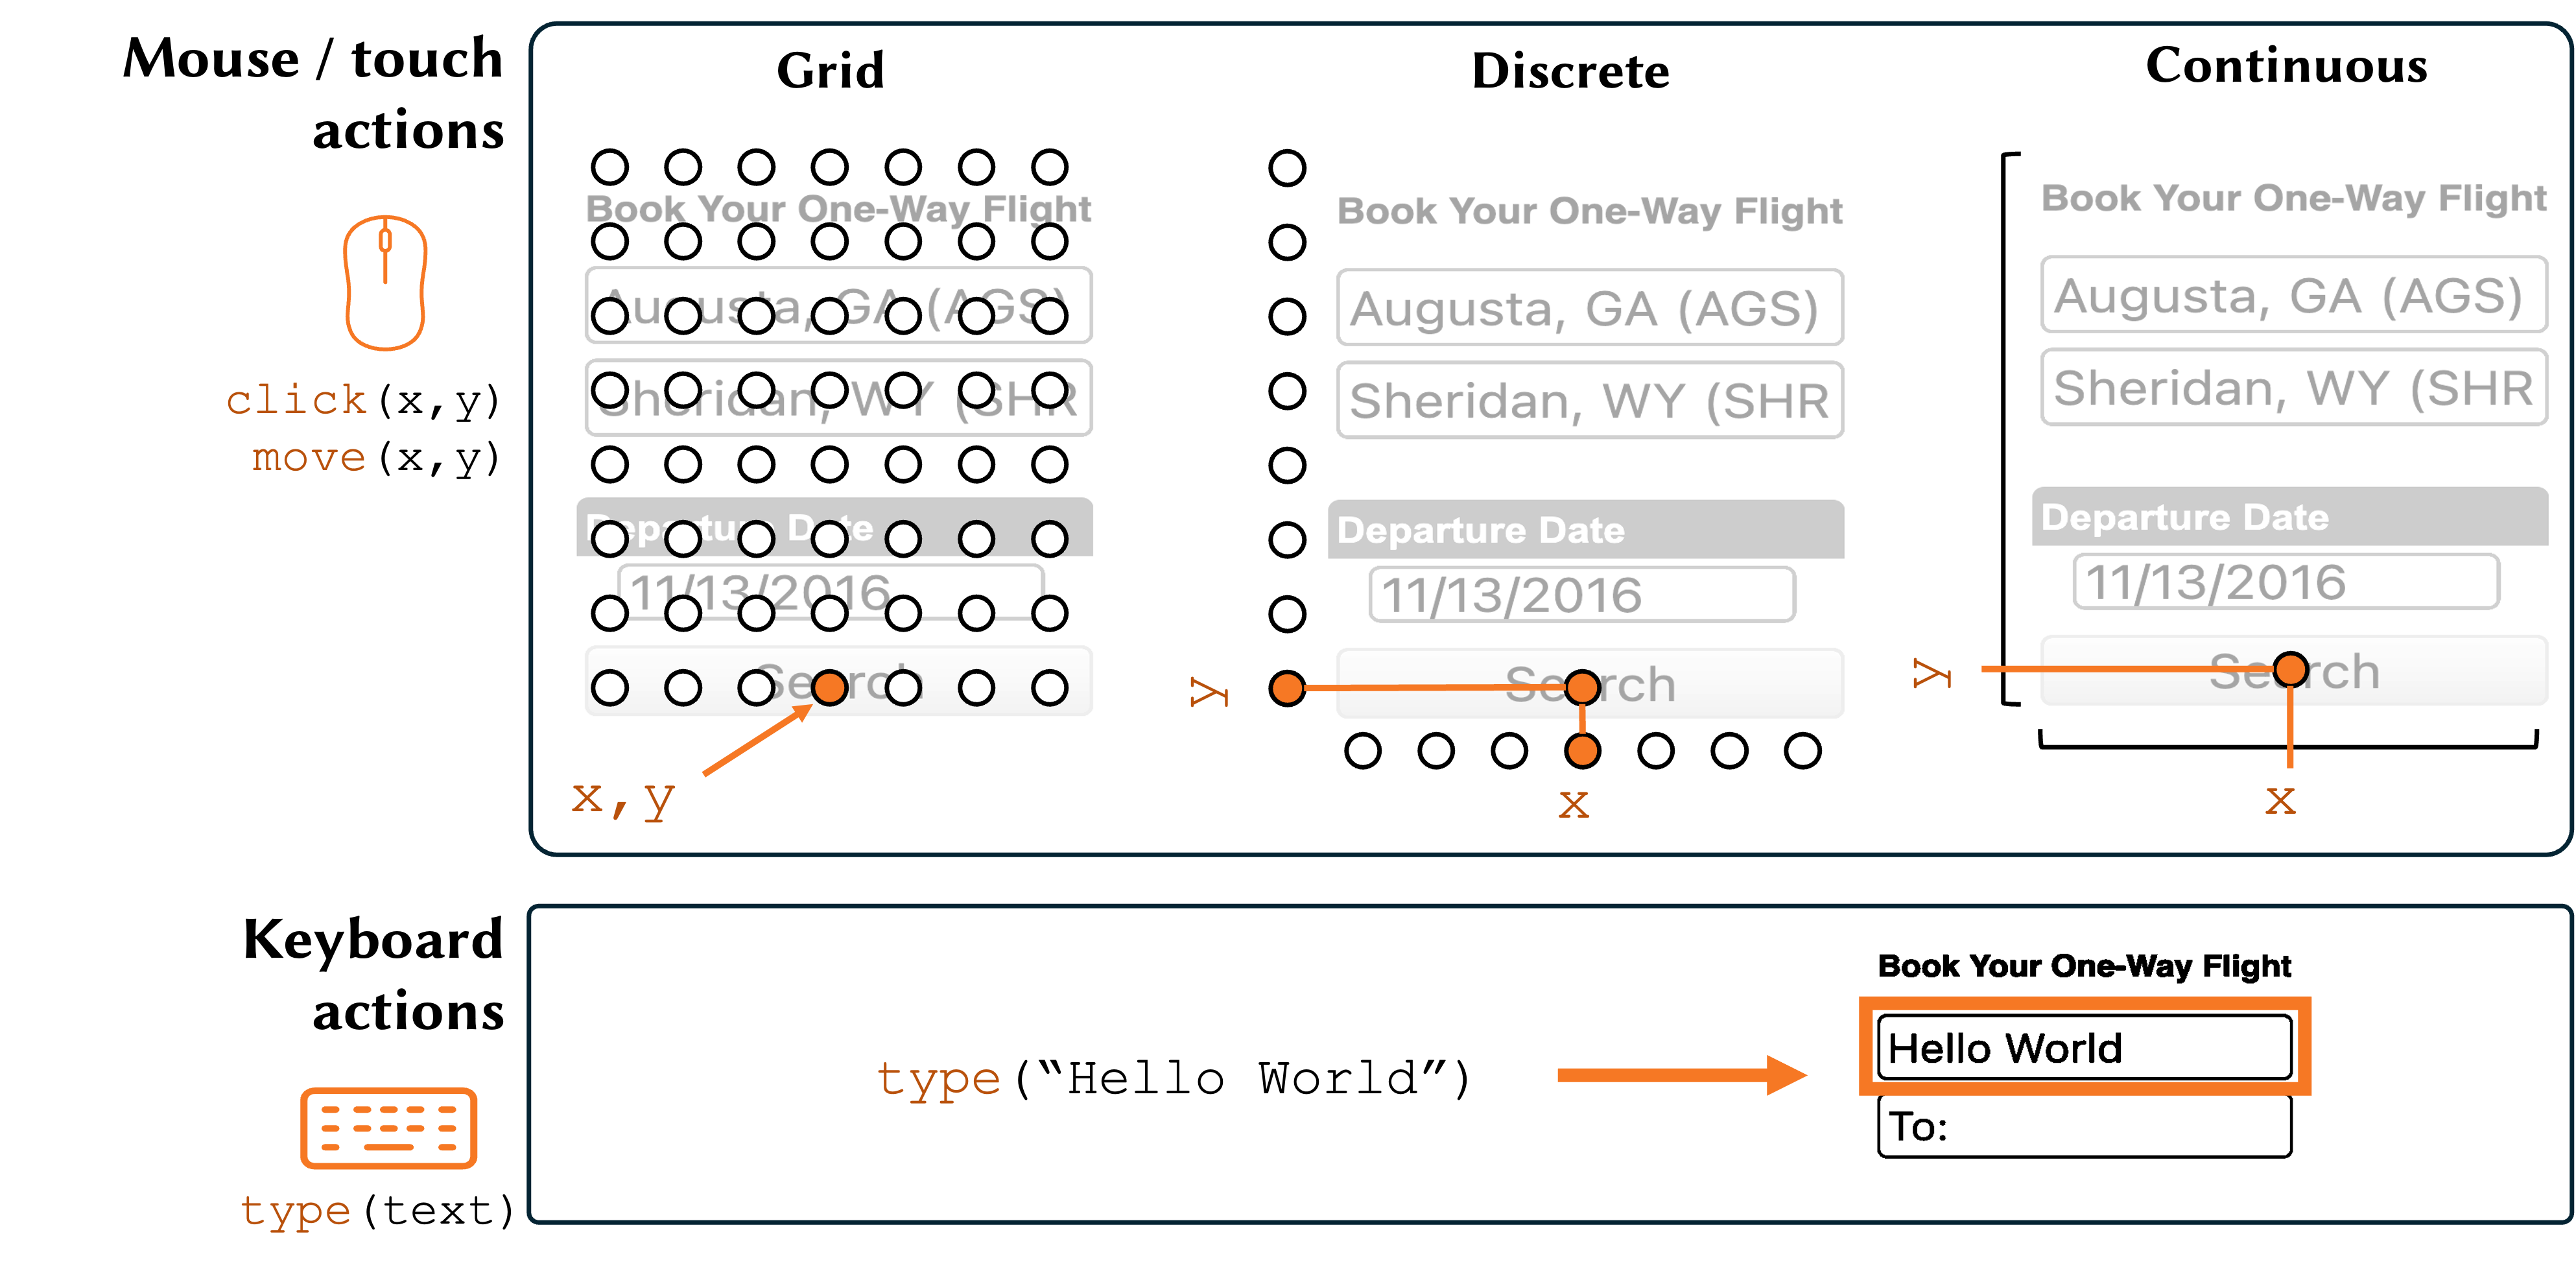
\includegraphics[width=0.65\linewidth]{figures/mouse_keyboard_action.png}
    \caption{Common mouse and keyboard actions, highlighting coordinate prediction.}
    \Description{Visualization of mouse and keyboard action modalities in agent control interfaces.
    The figure clarifies differences between common screen-coordinate prediction modes in user interface control. In the top section, three types of mouse or touch actions are shown using illustrative overlays: (1) grid-based prediction constrains clicks to fixed grid points, (2) discrete prediction allows selection from independent horizontal and vertical positions, and (3) continuous prediction enables unconstrained coordinate selection. These modes are visualized over a web form to highlight spatial precision. The bottom section shows a keyboard input scenario, where an agent types into a text box within a form interface. This comparison illustrates how action types differ in terms of input structure, spatial for mouse/touch, symbolic for keyboard, and supports the distinction between discrete and continuous action spaces.}
    \label{fig:mouse-keyboard-action}
\end{figure}

Keyboard actions (e.g., \texttt{type(text)}) are typically used to input text into a previously selected UI element.
While earlier methods relied on predefined text fragments \citepeg{humphreys_data-driven_2022} or extracted text from the instruction $i$ \citepeg{gur_learning_2019} as input, in most of the current systems, ACUs generate the text using a language model \citepeg{hong_cogagent_2024}, as this provides the required freedom to type diverse texts. 
%
% While free-text typing is a general-purpose action applicable across various applications, predicting predefined text fragments is often constrained to specific contexts and not used by general-purpose ACUs.
%
Beyond typing, keyboard actions are frequently used for special commands, such as navigating via pressing arrow keys \citepeg{li_zero-shot_2023} or using shortcuts such as \texttt{select all}, \texttt{copy}, or \texttt{paste} \citepeg{cho_caap_2024}.



\subsubsection{Direct UI Access}\label{sec:action_space_direct}

Direct UI access actions such as \texttt{click(e)} or \texttt{type(e, text)} target a specific UI element \texttt{e} observed by the agent.
Agents typically identify these elements \texttt{e} by either predicting unique identifiers like HTML \texttt{id} tags \citepeg{li_zero-shot_2023}, XPath\footnote{https://www.w3.org/TR/xpath-31/} descriptions \citep{kim_language_2023} (for an example of predicting \texttt{click(id=search)} based on \texttt{\(<\)button id="search"\(>\)} see \cref{fig:direct-action}), or by scoring and selecting from all visible elements \citepeg{jia_dom-q-net_2019, li_uinav_2024}.
%
\begin{figure}[b]
    \centering
    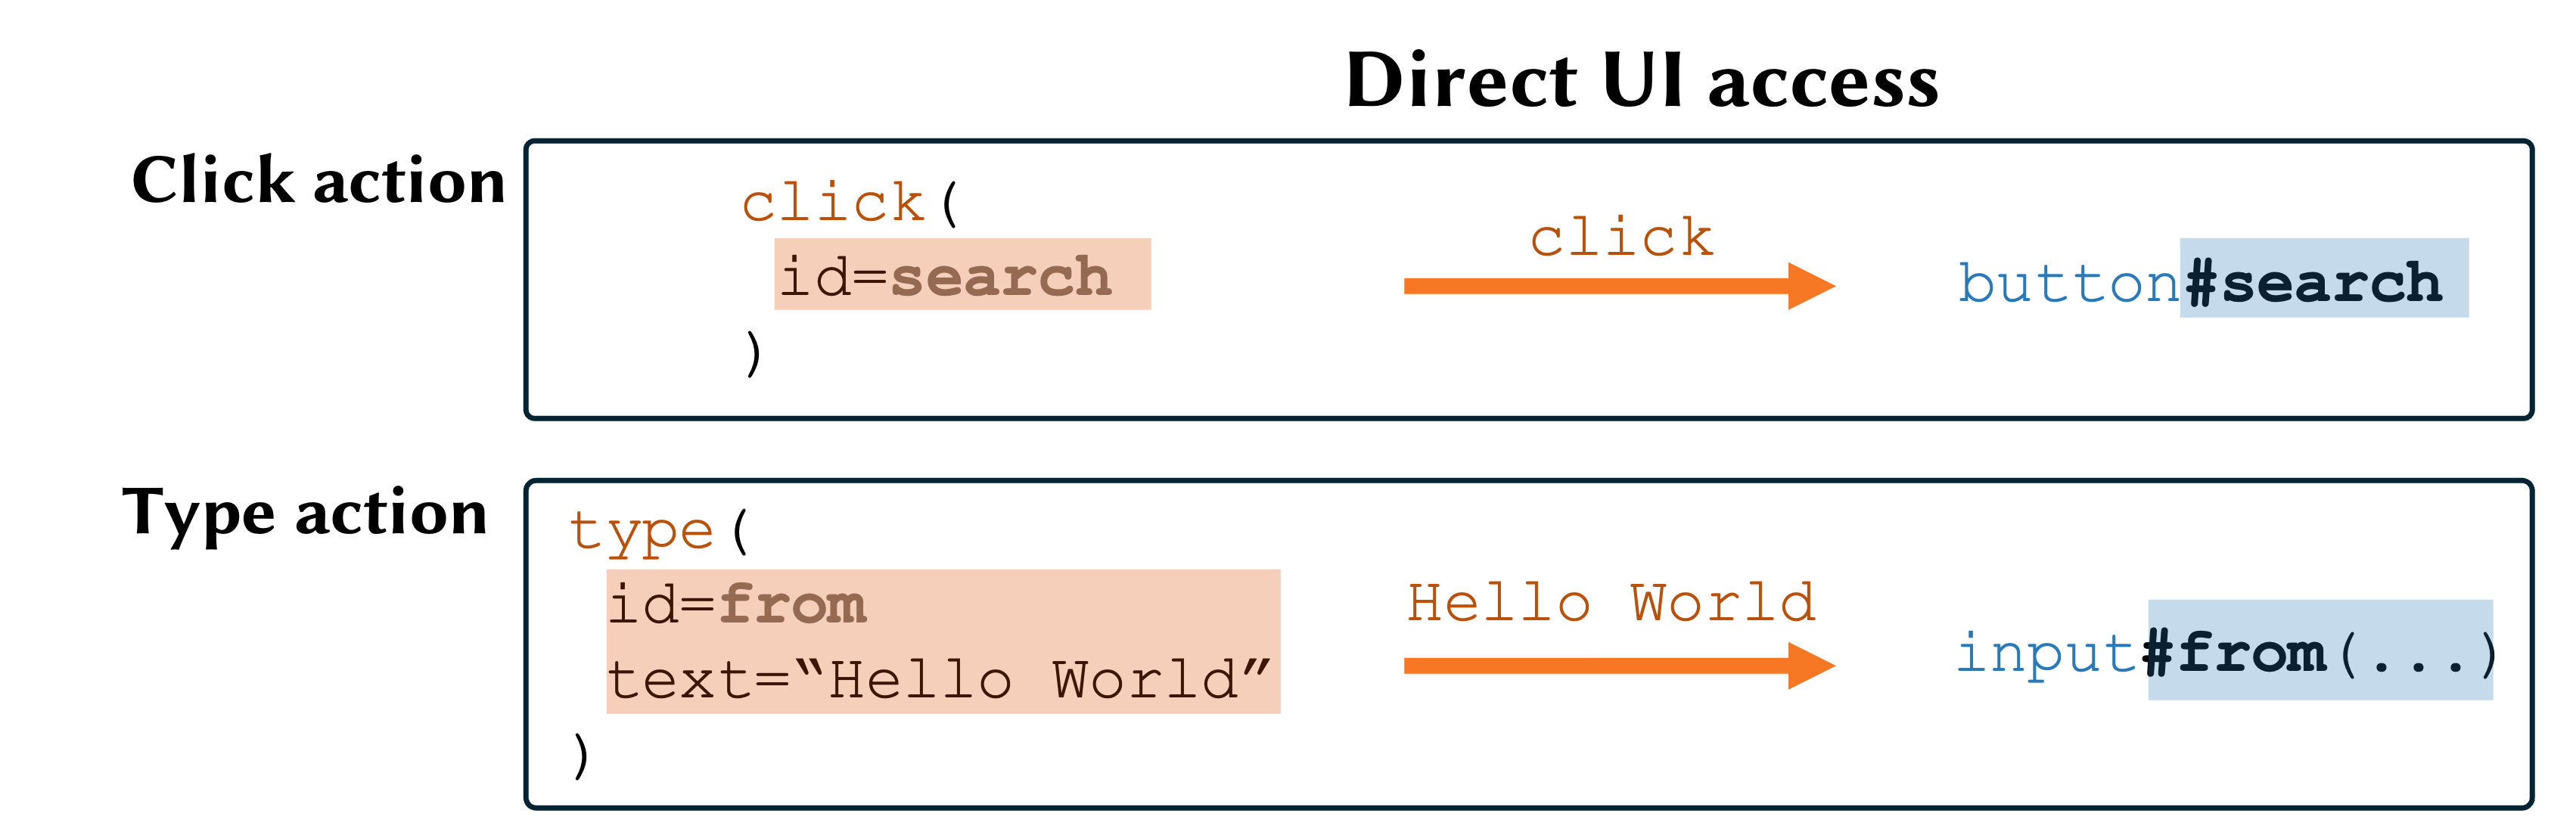
\includegraphics[width=0.6\linewidth]{figures/direct_action.png}
    \caption{Common direct UI access actions, referencing the HTML element by its \texttt{id} attribute.}
    \Description{The figure illustrates examples of direct UI access targeting HTML elements via their bolded \texttt{id} attributes. The first example demonstrates a click action where the function call specifies the \texttt{id} as ``search'' to trigger a button click. The second example shows a type action, in which the function call targets the input field with \texttt{id} equals ``form'' to enter the text ``Hello World.'' Arrows visually connect each function call to its respective HTML element, emphasizing the explicit mapping between the code and interface components.}
    \label{fig:direct-action}
\end{figure}

To simplify selection, agents may restrict referenceable elements to leaf nodes in the user interface tree \citepeg{liu_reinforcement_2018} or pre-filter them with an auxiliary model that can preselect potential candidate elements \citepeg{deng_mind2web_2023}. For specific tasks such as web navigation, agents may be limited by design to selecting hyperlinks only \citep{zaheer_learning_2022, chen_webvln_2024}.

After selecting an element, optional text input follows similar generation strategies as got keyboard input, including generating free-form text \citepeg{li_zero-shot_2023}, selecting predefined fragments \citepeg{shvo_appbuddy_2021}, or extracting text from the instruction \citepeg{jia_dom-q-net_2019}.

By classifying each reviewed ACU, we identify direct UI access as the most widely adopted action space in the literature (see Appendix~\cref{fig:action-space-dist}). We believe this dominance is due to its balance between generality and learnability. Unlike coordinate-based mouse or touch actions, which require fine-grained spatial reasoning and introduce high-dimensional prediction challenges, direct UI access operates over a lower-dimensional and semantically meaningful action space. By allowing agents to refer to structured element identifiers (e.g., \texttt{id}, XPath, or other selectors), this form of interaction abstracts away spatial complexity while still supporting a broad range of tasks.
However, as it requires an identifier for the UI elements, it is primarily compatible with text observations and, as discussed in the previous section, does therefore not scale well to the desktop domain.
Also, it typically only works well for simplified, well-structured UIs that are often not available for real-world use cases but common for earlier benchmarks (see \cref{sec:datasets}).


\subsubsection{Task-Tailored Actions}\label{sec:action_space_task}
Task-tailored actions are environment-specific commands for common operations.
For instance, \citet{wang_officebench_2024} define application-specific actions such as \texttt{create\_event} for a calendar application and \texttt{send\_email} for an email client.
These high-level actions reduce learning complexity as they typically correspond to an entire trajectory of clicking actions.
Nevertheless, the downside is that they require additional engineering as these subroutines are often hand-crafted \citepeg{wang_officebench_2024, tan_towards_2024}.

We consider most task-specific actions as a shortcut that might help to improve on narrowly designed benchmarks, but are not helpful for building general ACUs, especially when the actions are highly task-specific.
However, a few task-tailored actions demonstrate broader applicability and merit inclusion due to their capacity to generalize across tasks within a given domain.
For example, \citet{bonatti_windows_2024} define the action \texttt{open\_application}, which enables an agent to open and switch between applications on a Windows operating system. Similarly, \citet{nakano_webgpt_2022} define a \texttt{search} action, which allows the agent to navigate to specific text positions within a website. These actions exemplify a favorable trade-off between general-purpose utility and domain-relevant specialization, particularly when integrated with more comprehensive action spaces.

\subsubsection{Executable Code}\label{sec:action_space_code}
Agents may also generate code, executed by interpreters like Python or Bash.
Executable code varies in its structure and the level of abstraction provided by its application programming interface (API):

\begin{description}
    \item[Structure] of generated code: \hfill
        \begin{description}
            \item[Straight-line code] consists of a sequence of statements without control flow \citepeg{tao_webwise_2023}. It is akin to predicting a single or multiple actions.
            \item[Control-flow code] includes control flow mechanisms such as conditional statements (e.g., \texttt{if}), loops (e.g., \texttt{for}), and function definitions. Complex code can represent the agent's entire execution plan \citep{sun_adaplanner_2023}, where the agent dynamically adjusts its plan based on precondition checks failing.
        \end{description}
    \item[API abstraction level] utilized by generated code: \hfill
        \begin{description}
            \item[General-purpose API:]
                Some agents use an API with functions akin to general-purpose actions like clicking elements or screen coordinates. For example, \citet{gur_real-world_2024} use the Selenium web driver API\footnote{\url{https://www.selenium.dev/documentation/webdriver/}} to provide such low-level interactions.
            \item[Task-tailored API:]
                Other agents use an API of hand-engineered functions tailored to tasks. For example, \citet{guo_pptc_2024} define functions like \texttt{insert\_rounded\_rectangle(...)} for their PowerPoint agent.
        \end{description}
\end{description}

See Appendix \cref{fig:action-space-code} for both code structure and API abstraction examples.
Executable code is generated using either general foundation models \citepeg{guo_pptc_2024} or specialized models \citepeg{gur_real-world_2024}. Foundation models often come pre-trained on well-established APIs like Selenium web driver, while hand-engineered functions are typically introduced through contextual prompts or, alternatively, by using an API selector to first retrieve relevant functions \citep{song_restgpt_2023}.

An open question is the benefits of using executable code over other action types.
\citet{chen_program_2023} and \citet{gao_pal_2023} found that producing straight-line code instead of predicting actions as strings can reduce hallucinations when using GPT-3. 
However, \citet{assouel_unsolved_2023} suggested that this advantage disappears when using GPT-4, indicating that the benefits of executable code over other action types diminish with more advanced models.

\subsubsection{Action Grounding}\label{sec:action_space_grounding}
Action grounding  $a_t^* \rightarrow a_t$ refers to the process of converting an abstract action, such as \texttt{click submit button}, into an executable action, such as \texttt{click(e)}, where \texttt{e} represents the specific UI element. Grounding is typically required when a text foundation model generates an abstract, text-based plan that must be transformed into a sequence of executable actions \citepeg{gao_assistgui_2024, kim_language_2023}.
% 
Two common strategies include:

\begin{description}
    \item[Prediction-based grounding:] 
        Given an abstract action, a grounding model predicts the corresponding UI element. For example, for the abstract action \texttt{navigate to settings}, \citet{li_mapping_2020} predict \texttt{click(e)} where \texttt{e} refers to the settings app icon.
    \item[Rule-based grounding:] 
        A rule-based module matches an abstract action $a_t^*$ to the actionable UI element. For example, \citet{song_visiontasker_2024} use text matching rules to achieve this mapping, whereas \citet{lee_explore_2023} first predict abstract \emph{template} actions containing placeholders (e.g., \texttt{click(text=``[contact\_name]'')}), followed by rule-based grounding substituting the placeholders with context-specific values derived from the user instruction $i$.
\end{description}

Grounding is not limited to textual models but is also used in vision-based agents.
These vision-based agents rely on grounding because current vision models struggle to predict screen coordinates accurately. Several strategies for grounding in vision models have been explored and discussed by \citet{zheng_gpt-4vision_2024}.
The most successful one is \emph{set-of-mark} prompting \citep{yang_set--mark_2023}, where actionable elements are annotated with bounding boxes and unique identifiers, enabling the agent to access them directly using the identifier instead of relying on coordinate prediction.
However, this prompting strategy requires identifying the actionable elements, which is done by either using an additional textual screen representation with positional data \citepeg{zheng_gpt-4vision_2024,li_appagent_2024,zhang_appagent_2023} or extracting them from the screenshot via a specialized model \citepeg{lu_omniparser_2024}. 
Although the latter approach offers flexibility, it is often imprecise, leading to suboptimal performance \citep{bonatti_windows_2024}.

Despite the success of set-of-mark prompting, we posit that this grounding step may be a temporary workaround, designed to compensate for the limitations of current vision foundation models, which have not yet been trained sufficiently to predict screen coordinates directly. Recent studies suggest that learning visual grounding via coordinate prediction is feasible and straightforward \citep{dardouri_visual_2024, cheng_seeclick_2024} and may eventually render the need for set-of-mark prompting unnecessary.



\subsubsection{Recommendations}
%
\begin{figure}[t]
    \centering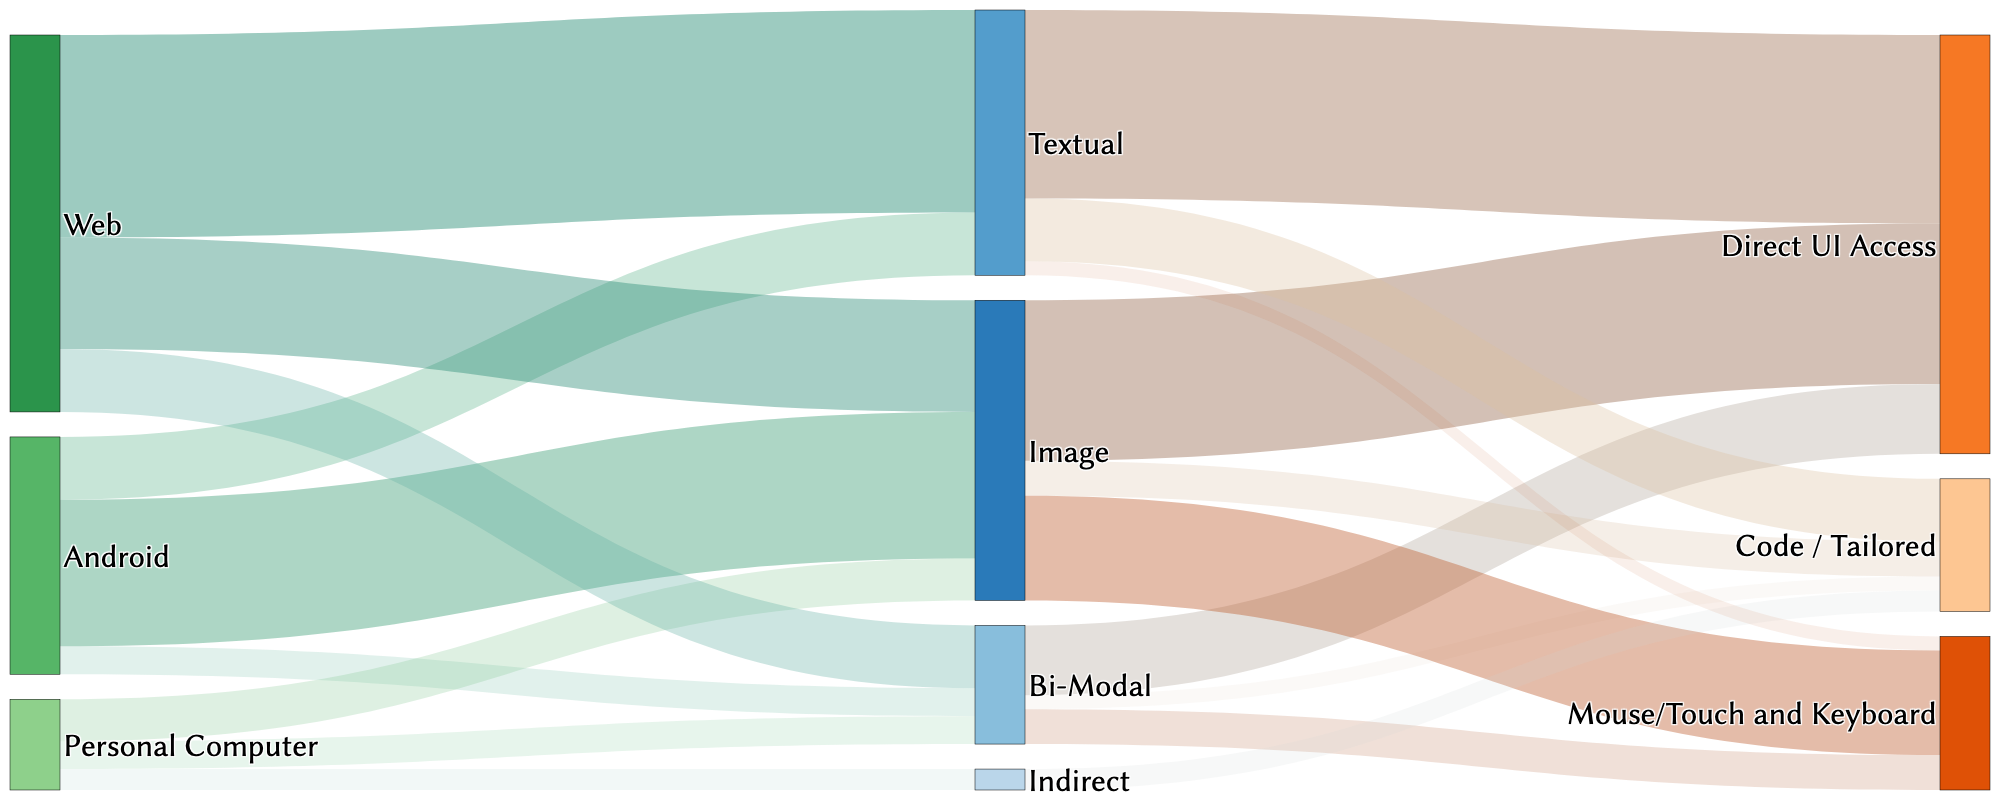
\includegraphics[width=1\linewidth]{figures/data/doa_sankey.png}
    \caption{Sankey diagram showing the connections between domains (left) and observation spaces (middle), and between observation and action spaces (right). The path width represents the number of papers within this survey associated with the corresponding topic.}
    \Description{A Sankey diagram with three columns depicting the relationships among surveyed research papers across domains, observation types, and action types. The left column enumerates the domains: Web, Android, and personal computer. The middle column presents observation types categorized as Image, textual, bi-modal, and indirect. The right column displays action types, including direct user interface (UI) access, mouse/touch and keyboard input, and code/tailored actions. Flows connect domains to observation types and subsequently to action types, with flow widths proportional to the number of papers associated with each connection. The strongest flows from domains to observations are from Web to textual data, Android to image, and Web to image. Among observation-to-action connections, the most prominent flows are from textual and image observations to direct UI access, with notable flows from image observations to mouse/touch and keyboard actions. This visualization provides a quantitative summary of prevailing research focuses within the surveyed literature.}
    \label{fig:domain-os-as-sankey}
\end{figure}


Different action types demand distinct observational inputs.
Coordinate-based actions (e.g., mouse clicks) depend on spatial information, whereas direct UI actions (e.g., button presses) must be able to reference UI elements. 
Consequently, coordinate-based actions naturally align with visual input, while element-based actions align with text-based input.

Nevertheless, our analysis shows many deviations from this expected alignment through modality bridging.
For instance, many vision-based agents employ direct UI access actions (see \cref{fig:domain-os-as-sankey}).
While such strategies can be effective, we argue that they are short-term workarounds tailored to existing technological constraints, introducing unnecessary long-term architectural complexity.

Historically, during the dominance of text-only LLMs, many ACUs converted screenshots into textual representations to maintain compatibility \citepeg{song_visiontasker_2024,wen_autodroid_2024}.  More recently, techniques such as set-of-mark prompting have been adopted to compensate for shortcomings in precise coordinate prediction \citepeg{zheng_gpt-4vision_2024,zhang_appagent_2023}.
These workarounds are likely to diminish in relevance as vision foundation models improve in spatial and semantic grounding.

Expanding on the premise that image-based observations offer a more coherent and spatially continuous representation of the user interface, we propose that \textbf{versatile ACUs should rely on mouse, touch, and keyboard actions} as these actions align naturally with visual observations.
Moreover, these actions can still be combined with higher-level subroutines (e.g., application switching) that abstract common interaction patterns into single actions.

\section{Agent Perspective}\label{sec:conceptional_view}

While previous sections described the agent's external environment and interactions, this section examines the internal structure of ACUs.
Here, we focus on two prevalent agent types: \emph{Foundation agents} (based on foundation models) and \emph{specialized agents} (based on domain-specific design).

\begin{description}
    \item[Foundation Agent:] \label{sec:foundation_agent}
    A foundation agent \citepeg{zheng_gpt-4vision_2024} uses a \emph{general pre-trained} foundation model (such as an LLM or VLM) as its policy $\pi$. While currently dominated by LLMs and VLMs, this category encompasses any architecture leveraging broad pre-training for zero-shot or few-shot transfer, including vision-language-action (VLA) models or diffusion models. These agents employ the model's broad knowledge and in-context learning capabilities for \emph{episodic improvement} (see \cref{sec:learning_strategy_pretraining,sec:episodic_improvement}).
    For example, a text-based foundation model receives a textual observation $o_t$ alongside a prompt specifying its role as agent, a description of available UI actions $\mathcal{A}$, and the instruction $i$. The model then \emph{generates} an action $a_t$ that is executed in the environment.
    %During each episode, the agent typically accumulates a \emph{history} of past observations and actions to provide additional contextual information to the foundation model as needed (see \cref{sec:agent_policy}).
    \item[Specialized Agent:] \label{sec:reinforce_agent}
    A specialized agent \citepeg{humphreys_data-driven_2022} employs a \emph{custom} network architecture as its policy $\pi$, which \emph{predicts} actions $a_t \in \mathcal{A}$ based on a given observation $o_t$ and instruction $i$, relying on the possibilities of the predefined output options.
    For example, the architecture might process an image $o_t$ and a text instruction $i$ as inputs through encoder networks and predict logits for each action type (such as \texttt{clicking}) alongside additional outputs (such as screen coordinates \texttt{(x,y)}). 
    %To track the past, observations are continuously aggregated in an internal Markov \emph{state}.
    Learning typically involves \emph{environment learning} techniques such as reinforcement learning (see \cref{sec:environment_adaption}).
\end{description}

Specialized agents work particularly well on narrow tasks and when the task conditioning of humans (the instruction) is limited (e.g., fill out a simple form given a user ID). In such cases, specialized agents often perform robustly and are computationally efficient due to their smaller parameter count \citepeg{humphreys_data-driven_2022}.
However, in multi-step tasks with diverse observation spaces or strong instruction-based conditioning, agents clearly benefit from general pre-training and reasoning techniques such as Chain-of-Thought (CoT) \citepeg{zhou_webarena_2024}. 

\Cref{table:two-main-agents} summarizes the key characteristics of the two common agent designs, highlighting their differences in architecture, action type, memory of information from past episodes, and learning strategy.

\begin{table}
    \caption{Properties of the two common ACU types.}
    \label{table:two-main-agents}
    \begin{tabular}{lllll}
    \toprule
   \textbf{ACU Agent Types } & \textbf{Architecture}   & \textbf{Action}  & \textbf{Memory}  & \textbf{Learning Strategy} \\ 
    \midrule
    Foundation agent & LLM / VLM               & Generation       & history-based  & General + Episodic \\
    Specialized agent  & Custom                  & Prediction       & state-based    & Environment learning  \\ 
    \bottomrule
    \end{tabular}
\end{table}

\subsection{Policy -- How to Act}\label{sec:agent_policy}
The policy $\pi$ defines how an agent selects actions \citep[Chapter~1.3]{sutton_reinforcement_2018}. For computer control, we distinguish three types of policies: Memoryless policies that act only on the current input; history-based policies that use explicit past observation and/or action sequences; and state-based policies that aggregate information about the past in an internal memory. 
%Among these, history-based and state-based policies leverage distinct types of memory to track past observations and/or actions.
Among them, history-based policies are the main research focus in the surveyed reviews, with almost $60$ out of the reviewed $87$ ACUs using some form of history in their policy (see Appendix \cref{fig:policy-dist} and \cref{tab:agent_literature}).
%The distribution of these policies across agents analyzed in this review shows in \cref{fig:policy-dist} (for a detailed association to publications, refer to \cref{tab:agent_literature}).

\subsubsection{Memoryless Policies}\label{sec:agent_policy_memoryless}
Memoryless policies \citepeg{chen_webvln_2024} ignore past observations and actions and act solely on the current observation $o_t$:
\begin{equation}
a_t \sim \pi(\ \cdot\ |\ o_t,\ i\ ) \label{eq:memoryless-policy}
\end{equation}

Memoryless policies are often insufficient for real-world control scenarios where context across time is critical and selecting an appropriate next action $a_t$ requires information about past observations $o_{t-n}, ..., o_{t-1}$ and/or actions $a_{t-n}, ..., a_{t-1}$. 
For instance, in the context of purchasing multiple items from an online store, an agent must remember which items were already added to the shopping cart.
% Therefore, state-of-the-art agents utilize more complex policies.
Still, since memoryless can be sufficient for specific tasks, their simplicity is sometimes leveraged in model design \citepeg{shvo_appbuddy_2021}.

\subsubsection{History-based Policies}\label{sec:agent_policy_history}
History-based policies track the past by adding observations and actions in a continuously growing sequence, called history $h_t=\left(o_{0},\hdots,o_{t-1},a_{0},\hdots,a_{t-1}\right)$ \citepeg{zheng_gpt-4vision_2024}.
For example, a vision-only agent's history consists of all the screenshots it perceived and the actions it performed during an episode. When predicting the next action $a_t$, the agent retrieves relevant information from its history $h_t$:
%
\begin{equation}
a_t \sim \pi(\ \cdot\ |\ o_t,\ i,\ h_t\ ) \label{eq:history-based-policy}
\end{equation}

Foundation agents commonly follow this pattern, as foundation models typically come with a context window to track past information, a specific instance of a policy history.
A key challenge with history-based approaches lies in the high dimensionality of observations $o_t$ (often screenshots or long textual descriptions). They either do not fit into the limited context windows of foundation models or, if they fit, they are computationally very expensive due to the large amount of required tokens.
Therefore, the history $h_t$ is often approximated as $h_t^*$. Common simplifications include:

\begin{description}
    \item[Actions only:] Keep only the past actions $h_t^*=\left(a_0,\hdots,a_{t-1}\right)$ and discard the observations \citepeg{zheng_gpt-4vision_2024}. In extreme cases, retain only the last action $h_t^*=\left(a_{t-1}\right)$ \citepeg{gao_assistgui_2024}.
    \item[Selective observations] Retain certain previous observations $o_{<t}$, such as keeping the last two screenshots with all actions as $h_t^*=\left(o_{t-2},o_{t-1},a_0,\hdots,a_{t-1}\right)$ \citep{furuta_multimodal_2024}.
    \item[Embedded summaries:] Create embeddings of the last observations $h_t^*=\left(\tilde{o}_{t-4},\hdots,\tilde{o}_{t-1},a_0,\hdots,a_{t-1}\right)$ \citep{lu_gui_2024}.
    \item[Text summaries:] Summarize past observations into text, enabling to keep the entire summarized observation history alongside raw actions $h_t^*=\left(\tilde{o}_{0},\hdots,\tilde{o}_{t-1},a_0,\hdots, a_{t-1}\right)$ \citep{zheng_synapse_2024}.
\end{description}

These strategies reduce token usage but risk omitting essential information, as the function for reducing information is not optimized for the given task. While suitable for simple GUIs, they are likely to limit performance in tasks requiring longer-term reasoning.

\subsubsection{State-based Policies}\label{sec:agent_policy_state}
In contrast, state-based policies rely on a compact internal memory $m_t$, often referred to as a Markov state, that is of fixed dimensionality and used during the action selection process \citepeg{humphreys_data-driven_2022}:
%
\begin{equation}
a_t \sim \pi(\ \cdot\ |\ o_t,\ i,\ m_t\ ) \label{eq:state-based-policy}
\end{equation}
%
This internal state $m_t$ is updated at each time step via a deterministic state-update function, typically of the form $m_{t+1}=f_m(o_{t},m_{t})$.
In practice, $f_m$ is commonly implemented as a learnable function, such as a recurrent neural network, enabling the agent to track task-relevant aspects of the history in a compressed representation for improved decision-making \citepeg{humphreys_data-driven_2022}.

While foundation models typically employ history-based policies, specialized agents often rely on state-based policies.
A notable exception is \citet{zhang_appagent_2023}, who propose a foundation agent with a state-based policy using an external \emph{text-based} state $m_t$. The foundation model not only generates the next action $a_t$ but also the next state $m_{t+1}$ given the current state $m_{t}$ and observation $o_t$, effectively operating as both policy and state-update function.

\subsubsection{Mixed Policies}\label{sec:agent_policy_mixed}
Mixed policies are hybrid approaches that combine history and state.
For example, \citet{bonatti_windows_2024} prompt their internal foundation model with the past actions and the last observation $h_t^*=\left(o_{t-1},a_0,\hdots, a_{t-1}\right)$, while keeping an external text-based state $m_t$.
Similarly, \citet{iki_berts_2022} feed the current observation $o_t$, the last action $h_t^*=\left(a_{t-1}\right)$, and an external text-based state $m_{t}$ into a fine-tuned model to predict the next action $a_t$ as well as state $m_{t+1}$.

% Zhang et al. \cite{zhang_appagent_2023}, use a foundation, state-based agent. Their foundation model generates the next action and a text-based summary given the current observation $o_t$ and the previous summary; the summary is essentially a text-based state.

\subsubsection{Recommendations}
Most state-of-the-art approaches leverage foundation models that use history-based policies.
Nevertheless, processing the full, unfiltered episode history at every decision step is computationally inefficient and, in many cases, infeasible. This limitation necessitates some form of history simplification for history-based policies. 
A common approach involves retaining only past actions while discarding observations. Although effective for current benchmarks, this method deliberately omits observation information that is essential for solving more complex tasks requiring reasoning over temporally distributed observations.

Other history simplification strategies are either manually crafted \citepeg{cho_caap_2024} or based on generic summarization models \citepeg{zheng_synapse_2024}, both lacking adaptability to environments.
We posit that the ability to act effectively in complex environments inherently involves the capacity to learn what historical information is relevant and what can be safely ignored. Therefore, we argue that \textbf{history simplification should be a learnable component of the agent}, integral to achieving robust and generalizable behavior for complex tasks. The literature on \emph{world models} is herein closely related (cp. \citet{ha2018world}, \citet{lecun_path_2022}, \citet{hafner2025mastering}).

Notably, specialized agents employ state-based policies, wherein past information is compressed into a Markovian state via a learnable state-update function.
This function can be interpreted as a form of learned history simplification.
This conceptual link between specialized and foundation agents, revealed by our taxonomy, may inspire future history simplification research for foundation agents.


\subsection{Learning Strategy - How to Learn to Act}\label{sec:learning_strategy}

An agent’s learning strategy can involve up to three stages (not all ACUs utilize every stage):

\begin{description}
    \item[General pre-training:] 
        The agent acquires broad, environment-agnostic knowledge. Examples include foundation models learning general-purpose capabilities or vision backbones learning image representations.
    \item[Environment learning:] 
        The agent learns to adapt to a specific computer environment. This involves explicit parameter (weight) updates or implicit methods, such as storing environment experiences for later retrieval.
    \item[Episodic improvement:] 
        The agent refines its performance within the current episode through methods such as instruction tuning or few-shot learning \citep{brown_language_2020}. Unlike the previous steps, this step does not result in persistent learning, as changes are discarded post-episode.
\end{description}

\Cref{fig:learning-flow} illustrates how these steps sequentially combine into learning strategies for both foundation and specialized agents.
Our analysis of learning strategies shows that the combination of general pre-training with prompting is the most common strategy (see Appendix~\Cref{fig:learning-strategy-dist}).
The following sections explore each learning step in detail, emphasizing current practices and highlighting exceptions.

\begin{figure}[t]
    \centering
    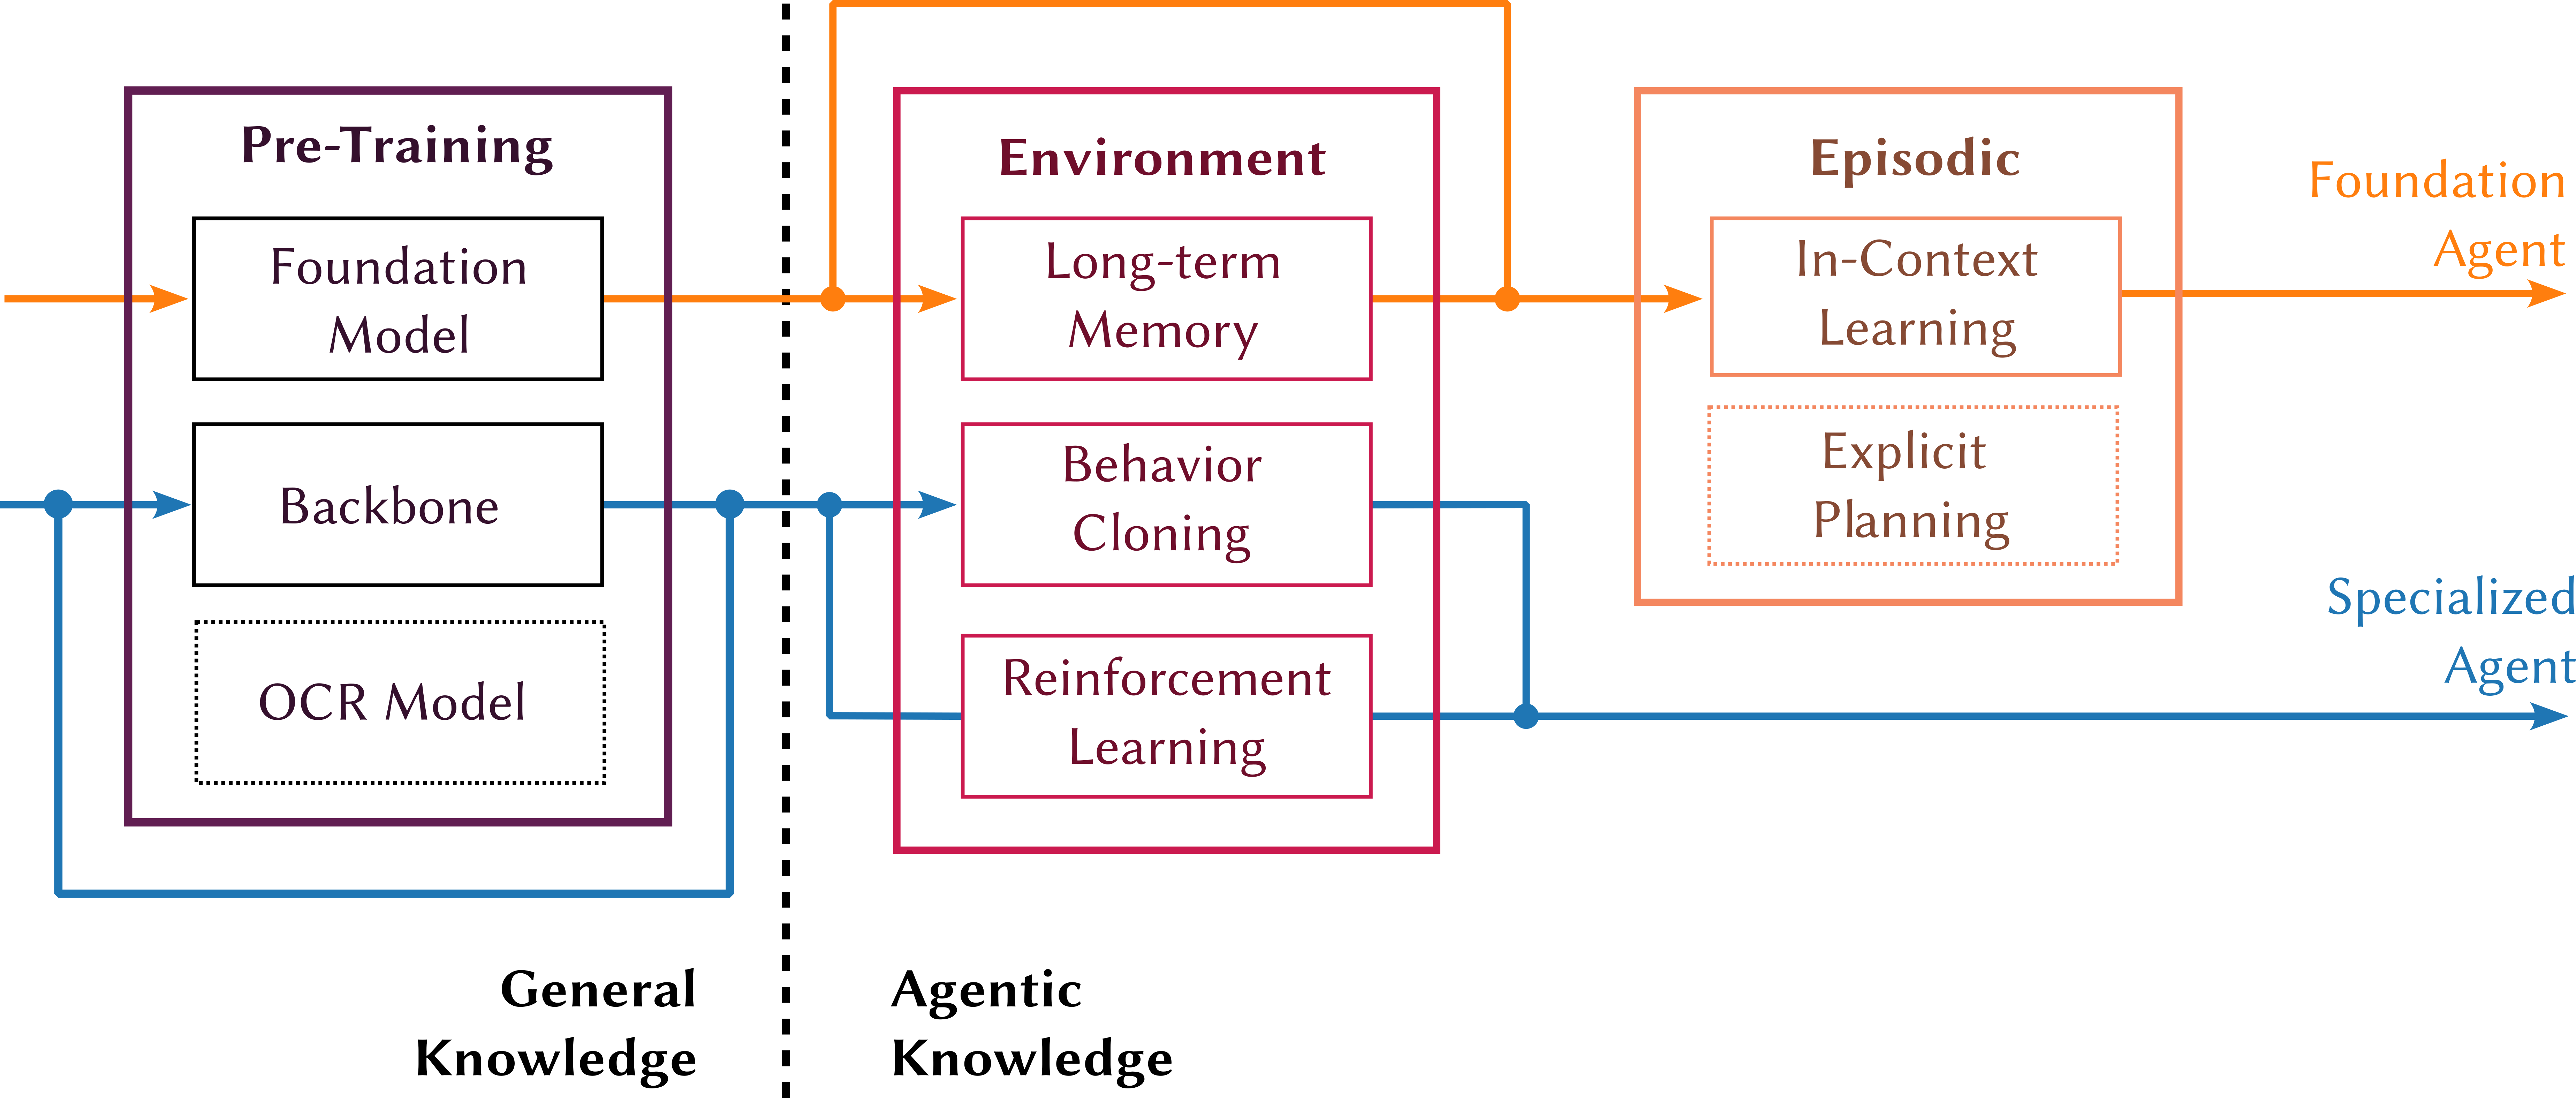
\includegraphics[width=0.95\linewidth]{figures/learning_flow_colored.png}
    \caption{Overview of learning steps and strategies: \emph{Pre-training} involves acquiring broad, environment-agnostic knowledge. \emph{Environment learning} and \emph{episodic improvement} hone a ACU's agentic capabilities. A combination of these steps defines a learning strategy. ACUs typically follow one of two strategies: (1) \emph{Specialized agents} (blue)  start from scratch or use a pre-trained backbone, learn to act in a specific environment through behavioral cloning (BC) or reinforcement learning (RL) ; (2) \emph{foundation agents} (orange) begin with a general-purpose foundation model, optionally storing successful episodes for future demonstration retrieval, and employ in-context learning.}
    \Description{The diagram depicts the learning strategies and typical training pathways of agents for computer use, organized into three main stages arranged from left to right: pre-training, environment learning, and episodic improvement. The pre-training stage includes the foundation model, backbone, and OCR model components and corresponds to general knowledge acquisition. The environment learning stage involves long-term memory, behavior cloning, and reinforcement learning, which together form agentic knowledge. The episodic improvement stage consists of in-context learning and explicit planning, aimed at refining agent performance in specific tasks. Two main learning strategies are illustrated by color-coded flow paths: foundation agents begin with the foundation model, optionally leverage components in the environment stage, and utilize in-context learning during episodic improvement, while specialized agents start from the backbone model or from scratch and rely on behavior cloning or reinforcement learning during environment learning. A dashed vertical line separates the pre-training phase from the subsequent stages, highlighting the transition from general to agentic knowledge. The figure emphasizes that foundation and specialized agents generally follow distinct and limited combinations of these training strategies.}

    \label{fig:learning-flow}
\end{figure}

\subsubsection{Leveraging General Pre-Training} \label{sec:learning_strategy_pretraining}
General pre-training serves as an initialization stage for an agent. This initial knowledge can be modified and adapted through \emph{environment learning} (e.g., fine-tuning, see \cref{sec:environment_adaption}) or preserved and utilized via \emph{episodic improvement} (e.g., prompting, see \cref{sec:episodic_improvement}).

Foundation agents primarily rely on the former approach. They leverage foundation models with broad knowledge and in-context learning capabilities \citep{brown_language_2020}. These capabilities can eliminate the need for environment-specific fine-tuning, allowing agents to operate in computer environments using only the foundation model's broad knowledge and instructions provided through prompts to adapt to specific environments \citepeg{kim_language_2023}.
For example, GPT-4 \citep{openai_gpt-4_2024}, when prompted as a web agent, can complete tasks such as filling out forms or navigating website links \citep{zheng_gpt-4vision_2024}.

In contrast, specialized agents are either trained from scratch \citepeg{humphreys_data-driven_2022} or initialized with a pre-trained backbone (e.g., an image encoder) to accelerate learning the observation space \citep{li_mug_2024}. These agents typically require additional fine-tuning to adapt to computer environments (see \cref{sec:environment_adaption}).
% 
The foundation model or backbone choice depends on the observation space, action space, and specific task requirements. For example, 
%\begin{itemize}
    %\item 
    \citet{zheng_gpt-4vision_2024} use GPT-4 \citep{openai_gpt-4_2024} as a multi-modal foundation model for their bi-modal agent.
    %\item 
    \citet{gur_real-world_2024} employ a coding-proficient foundation model \citep{chung_scaling_2022} to generate executable code.
    %\item 
    \citet{shaw_pixels_2023} fine-tune a vision backbone for their vision-based agent.
    %\item 
    \citet{iki_berts_2022} fine-tune a text backbone for their text-based agent.
    %\item 
    \citet{song_visiontasker_2024} use pre-trained object detection and OCR models to convert screenshots into text-based observations for direct UI access actions.
    %\item 
    \citet{gur_real-world_2024} pre-train an LLM from scratch only on HTML data while utilizing an HTML-specific local and global attention mechanism.
%\end{itemize}

\subsubsection{Environment Learning}\label{sec:environment_adaption}
Environment learning involves adaptation to computer environments through experience. Three main approaches are used: \emph{reinforcement learning}, \emph{behavioral cloning}, and \emph{long-term memory}. Among them, behavioral cloning is the most frequently used strategy (see Appendix~\Cref{fig:environment-adaption-dist}). 

Many foundation agents bypass the environment learning step, relying solely on their pre-trained, out-of-the-box capabilities by using prompting strategies. While these capabilities can be remarkably effective \citepeg{zheng_gpt-4vision_2024}, the absence of environment learning limits these agents, as they lack mechanisms to adapt or improve their performance within specific computer environments.

\paragraph{Reinforcement Learning} \label{sec:environment_adaption_rl}

In reinforcement learning (RL), an agent acts in an environment and learns to maximize a cumulative reward by trial and error \citep{sutton_reinforcement_2018}.
For computer use tasks, such environments are hand-crafted simulations, called \emph{controlled environments}, designed to mimic real-world computer settings while providing a reward signal for guidance.
% 
RL has been implemented with various algorithms, including approximate policy iteration \citep{humphreys_data-driven_2022}, policy gradients \citep{shi_world_2017}, and bootstrapping with tree search \citep{shaw_pixels_2023}.

Agents in simpler environments may rely on brute-force exploration to learn directly from random behavior \citepeg{toyama_androidenv_2021, shvo_appbuddy_2021}.
However, in most computer environments, rewards are sparse as they are only given upon completing the assigned instruction $i$ \citepeg{shi_world_2017}, such as submitting a flight booking form after filling out \emph{all} details correctly.
Sparse rewards make learning from an initial random behavior often unsuccessful, as an agent is unlikely to predict a long action sequence by random chance \citep{humphreys_data-driven_2022}.
One strategy to mitigate sparse rewards is to begin by training an agent on human-labeled demonstrations (behavioral cloning), providing it with enough competence to start finding and learning from rewards \citepeg{shi_world_2017, humphreys_data-driven_2022}.
Relatedly, \citet{liu_reinforcement_2018} use human-labeled demonstrations to constrain the action space by defining sets of valid actions based on similarity to demonstrated actions, increasing the likelihood of reward discovery.

Without demonstrations, reward shaping \citep{ng1999policy} can artificially reduce sparsity by providing intermediate guidance, as shown by \citet{gur_learning_2019} and \citet{li_glider_2021}.
Alternatively, the task complexity can be adaptively adjusted. \citet{gur_environment_2021}, for instance, introduce a controlled environment that enables autonomous curriculum learning \citep{bengio2009curriculum} by automatically changing a task's complexity. Similarly, \citet{gur_learning_2019} employ curriculum learning by gradually moving an agent's starting point away from the goal state as it gains competence.

The key advantage of RL is its ability to autonomously explore environments and effectively navigate a dynamic dataset. However, RL's reliance on controlled environments limits its application to broad computer use tasks, as rewards must be defined and action consequences suppressed (i.e., ensure that actions within the simulation have no real-world consequences). The development of such environments can be very tedious, typically preventing current ACUs from acquiring broad knowledge by solely using RL.
Nevertheless, AndroidEnv \citep{toyama_androidenv_2021} combats this limitation by simulating a complete, virtual Android environment on top of which tasks can be configured by defining instructions and rewards.


\paragraph{Behavioral Cloning}\label{sec:environment_adaption_bc}

In behavioral cloning (BC) \citep{pomerleau_alvinn_1988}, an agent learns to mimic a shown behavior through supervised learning.
The shown behavior is usually a sequence of recorded observations and actions of a human completing a computer use task given an instruction \nolinebreak$i$.

Unlike RL, learning via BC does not require the agent to execute actions in the environment, making it applicable in \emph{uncontrolled} environments (trained based on observation-action pairs instead of a simulation). 
For example, \citet{zhang_you_2024} fine-tune a model on Android demonstrations from the work of \citet{rawles_android_2023}, while \citet{hong_cogagent_2024} combine Android demonstrations provided by \citet{rawles_android_2023} with Web demonstrations taken from the work of \citet{deng_mind2web_2023}.

BC methods vary in training strategies and data collection.
For example, \citet{gur_understanding_2023} train the entire model, \citet{hong_cogagent_2024} only update specific components, while \citet{li_effects_2024} use low-rank adaption \citep{hu_lora_2021} to fine-tune a foundation model.
Datasets are typically human-labeled \citepeg{humphreys_data-driven_2022}, but autonomous data collection methods also exist. For instance, \citet{furuta_multimodal_2024} use rejection sampling to identify successful trajectories from another agent's actions in a controlled environment, leveraging the environment’s rewards for validation. Similarly, \citet{lai_autowebglm_2024} iteratively collect successful demonstrations for improving their agent.

While BC can be used independently to train ACUs, it can also be used as a pre-trained step, with the ACU being fine-tuned afterward using RL to improve performance.
Typically, RL further enhances the agent by exploring aspects missing from the behavioral data. For instance, \citet{humphreys_data-driven_2022} demonstrate that after training their agent on $2.4$ million human-labeled actions, RL increases the task success rate from approximately $30\%$ to over $95\%$. 
Nonetheless, some agents rely entirely on BC, which can suffice for simpler tasks \citepeg{gur_understanding_2023}.

\paragraph{Long-Term Memory} \label{sec:environment_adaption_ltm}

\begin{figure}[b]
  \begin{subfigure}{0.49\linewidth}
    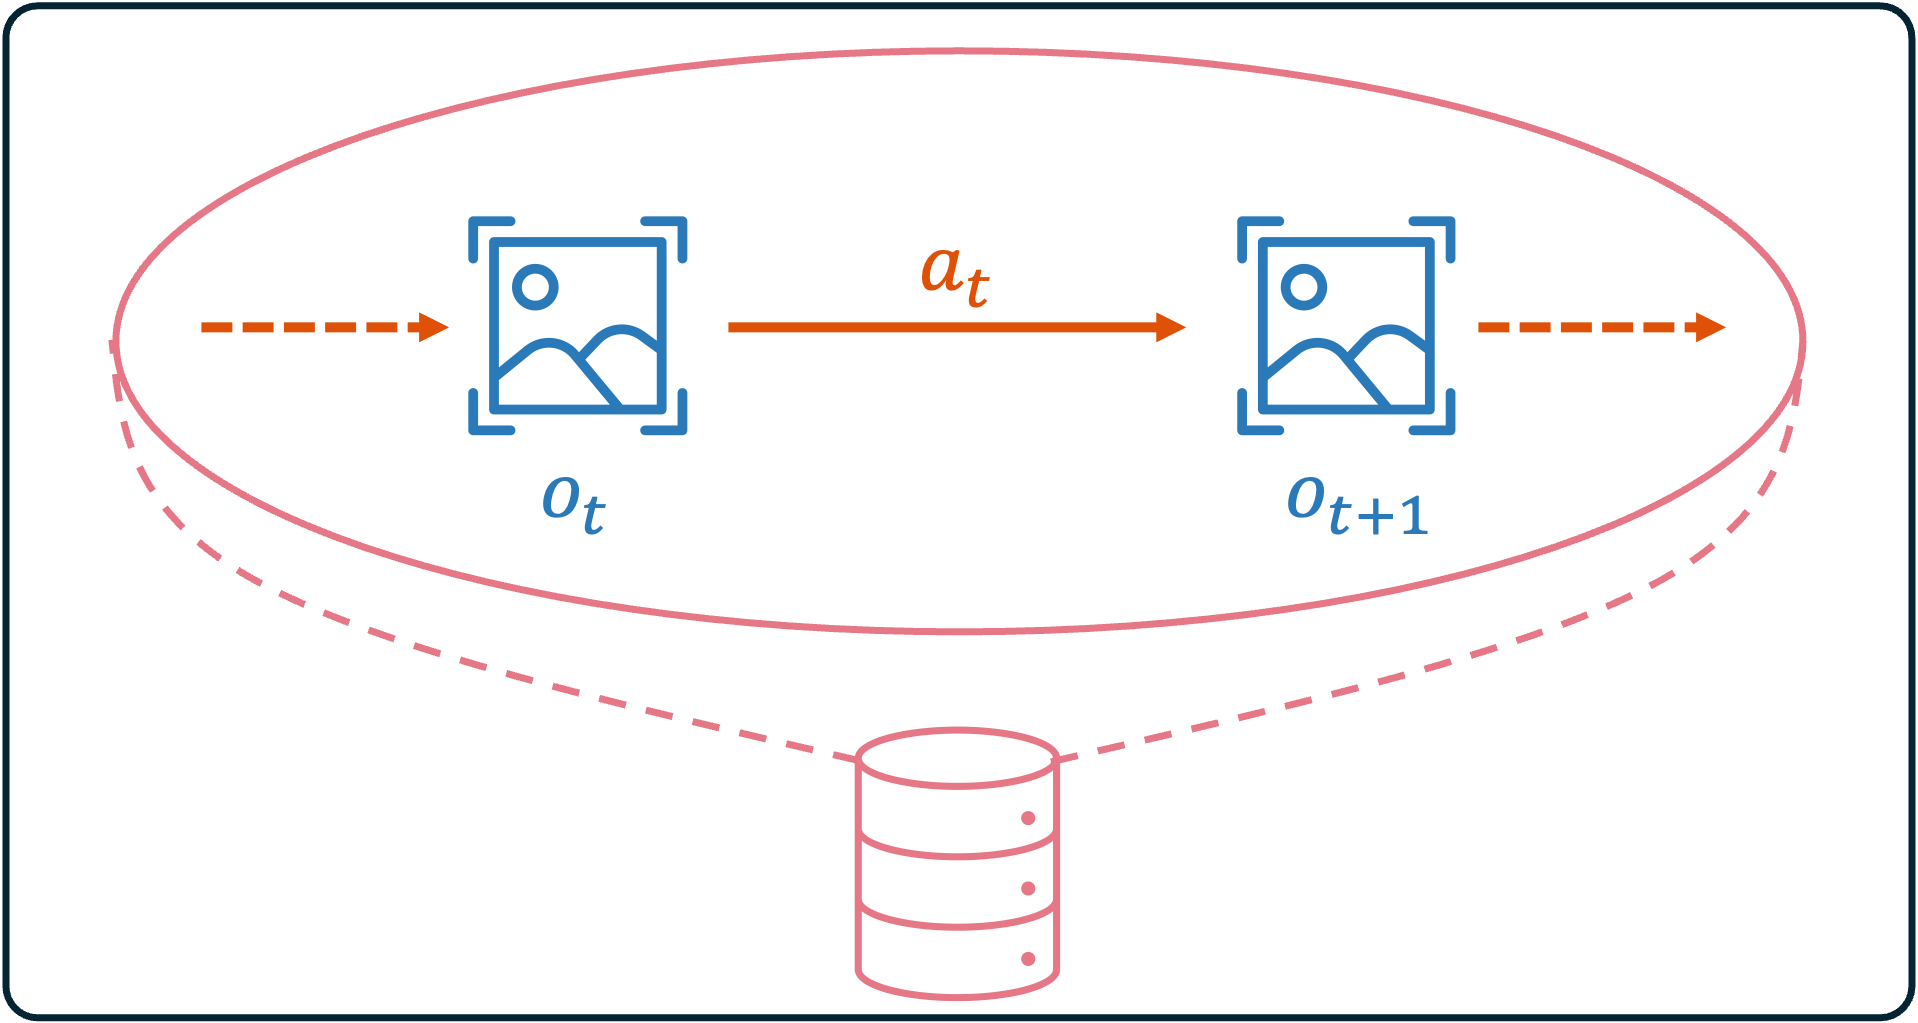
\includegraphics[width=\linewidth]{figures/few_shot_what_env.png}
    \caption{Memorize transitions $(o_t,a_t,o_{t+1})$}
    \label{fig:few_shot_what_env}
  \end{subfigure}
  \hfill
  \begin{subfigure}{0.49\linewidth}
    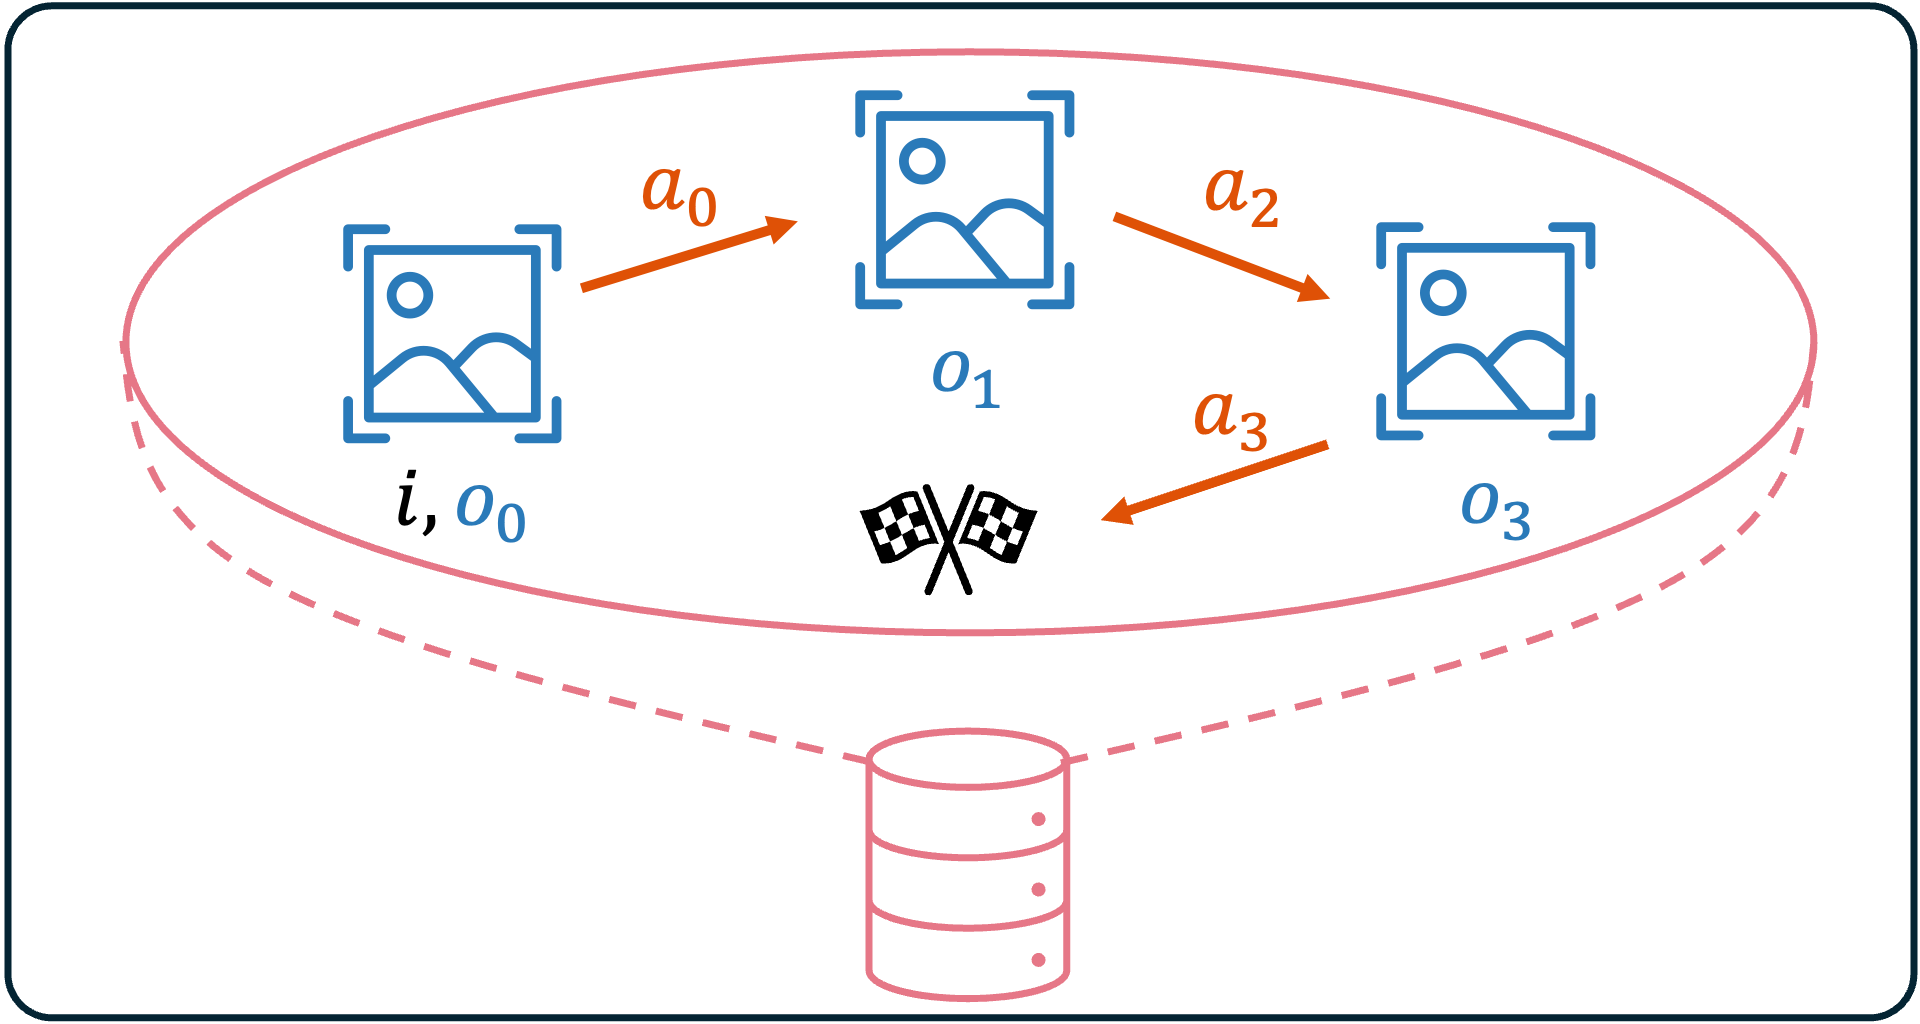
\includegraphics[width=\linewidth]{figures/few_shot_what_act.png}
    \caption{Memorize task demonstrations $(i,\tau)$}
    \label{fig:few_shot_what_act}
  \end{subfigure}
    \caption{Two kinds of experiences an agent can store in its long-term memory. (a) The agent memorizes the pre- and post-action observations as environment transitions $(o_t, a_t, o_{t+1})$. (b) The agent memorizes an instruction with a successful action-observation episode $(i, \tau)$}.
    \Description{This figure illustrates two conceptual approaches an agent can use to store experiences in long-term memory. The left panel shows storage of individual environment transitions as triplets consisting of the observation at time $t$, the action taken at time $t$, and the subsequent observation at time $t+1$. This emphasizes storing atomic transitions as discrete records. The right panel depicts storage of complete task trajectories, where an instruction is paired with the entire sequence of observations and actions from a successful episode. The figure uses a database symbol to represent the memory storage, highlighting that the left stores isolated transitions while the right stores full episodic trajectories.}
    \label{fig:few_shot_what}
\end{figure}

Foundation models exhibit strong few-shot learning capabilities \citep{brown_language_2020}, enabling foundation agents to enhance action prediction by incorporating successful demonstrations as examples directly into their context (see \cref{sec:episodic_improvement}).
This paradigm is also known as in-context learning (ICL).
Long-term memory extends ICL by first allowing the agent to execute and store successful trajectories in an external memory, and then later retrieve previous trajectories from this memory as examples of how a specific (sub-)task can be solved.
Importantly, since the examples are collected by the agent itself rather than provided by a human, the agent learns to improve its capabilities over time and adapts \emph{autonomously} to an environment (we discuss human prompt designs in the next section).
\cref{fig:few_shot_what} illustrates the two main types of experiences:

\begin{description}
    \item[Environment transitions:] 
        The agent memorizes environment transitions as triples ($o_t$, $a_t$, $o_{t+1}$), where $a_t$ represents the action taken, and $o_t,o_{t+1}$ capture the pre- and post-action observations, respectively. For example, the agent might store the consequence of its actions, such as ``clicking on the calculator app ($a_t$) on the home screen ($o_t$) opens the calculator app ($o_{t+1}$).'' \citet{wen_autodroid_2024} collect such transitions for Android apps in an offline phase by random exploration. They describe and summarize these transitions using an LLM, enabling the agent to enrich actionable elements with outcome information. For example, a \texttt{more options} button could be annotated to reveal specific hidden menu items, informing the agent what to expect if this button is clicked. Autonomous transition memories can also be combined with human demonstrations, as shown by \citet{zhang_appagent_2023} and \citet{li_appagent_2024}.
    \item[Task demonstrations:] 
        The agent memorizes task demonstrations by storing a tuple ($i$, $\tau_i$) containing the instruction $i$ and a successful demonstration $\tau_i=(o_{0},a_{0},\hdots,o_{t},a_{t})$ of solving $i$. Since only successful attempts are informative for the agent, the agent must have a mechanism to filter \emph{successful} trajectories. 
        % A common approach is to use a controlled environment's reward \citepeg{tao_webwise_2023} or human data \citepeg{li_appagent_2024}. Another approach is to use a foundation model to predict success \citepeg{}. 
        A common approach is to use a controlled environment's feedback and only to store trajectories that yield a high reward \citepeg{tao_webwise_2023}.
        To manage memory constraints, trajectories $\tau_i$ are typically simplified to $\tau_i^*=(\tilde{o}_0,a_0,\hdots,\tilde{o}_t,a_t)$ (where $\tilde{o}_i$ is a simplification of $o_i$) before being stored. 
        For instance, \citet{deng_multi-turn_2024} only keep the actions $\tau_i^*=(a_0,\hdots,a_t)$, while \citet{sun_adaplanner_2023} store the complete executable program that solves $i$.
        These simplifications mirror history simplifications ($h_t \rightarrow h_t^*$), as the history $h_t$ is a (partial) trajectory.
        An alternative approach for discovering successful trajectories is programming by demonstration. Here, a human supervises the agent, intervenes if necessary, and demonstrates the correct solution for $i$, enabling online learning. \citet{song_visiontasker_2024} propose this method to summarize the corrected behavior for future retrieval.
\end{description}

A limitation of memory-based approaches is their reliance on storing specific instances rather than learning abstract generalizations. To mitigate this, \citet{lee_explore_2023} organize memories into a graph where observations are nodes, actions are edges, and both are generalized to unify related experiences. For example, an action $a=$ \texttt{click(text=Bob)} is generalized to $a^*=$ \texttt{click(text=[contact name])}. When retrieving memories, the graph is searched, and parameterized actions are instantiated based on the current state $(o_t, i)$, grounding parameters like \texttt{[contact name]} to specific values.
However, it still remains challenging to map specific trajectory instances to general concepts and to later retrieve and adapt helpful general concepts for specific tasks.


\subsubsection{Episodic Improvement}\label{sec:episodic_improvement}
Episodic improvement refers to an agent's ability to enhance its performance within a single episode by reasoning over its current context, without retaining knowledge across episodes. This effectively trades test-time computing for improved task execution.

Foundation agents commonly achieve episodic improvement through in-context learning \citep{brown_language_2020}.
ICL encompasses techniques such as \emph{instruction tuning}, where guidance is provided to the model through the prompt, and few-shot learning, which gives examples of successful trajectories as \emph{demonstrations} to the agent.

In contrast, current specialized agents typically do not employ episodic improvement. However, analogous mechanisms exist, such as search-based planning in game-playing agents, which simulate future outcomes to guide action selection \citep{silver_mastering_go_2017}. Such approaches can be considered as a more traditional reasoning within agents.

\paragraph{In-Context Learning through Instruction Tuning} \label{sec:episodic_improvement_instruction}

Foundation models are often adapted to specific tasks through \emph{prompt engineering}.
Typically, these prompts are designed by humans to adapt a foundation model to specific environmental conditions \citepeg{zheng_gpt-4vision_2024} and can include guidance on valid actions, previous history, assumed roles, or intermediate reasoning steps.
\Cref{tab:in-context-learning} exemplifies some snippets taken from the (much longer) prompts in the literature (for more details, refer to Table 6 in Zheng at al.~\citep{zheng_gpt-4vision_2024}). 

While most prompts are human-authored, some methods automate prompt construction.
For example, \citet{sun_adaplanner_2023} uses a second model as a planner to autonomously generate prompts for the agent.
This strategy, known as \emph{self-prompting}, involves using multiple instances of the foundation model, each fulfilling different roles and interacting with one another through iterative prompting \citepeg{song_mmac-copilot_2024}.

With the rise of vision-language models, \emph{visual prompt engineering} has emerged. This includes techniques such as extending screenshots to incorporate user instructions \citep{lee_pix2struct_2023}, overlaying bounding boxes on actionable UI elements \citepeg{bonatti_windows_2024}, and adding unique identifiers for visual grounding \citepeg{zhang_ufo_2024}.

\begin{table}

    \caption{Example snippets of actual prompts.}
    \label{tab:in-context-learning}
     {\footnotesize
    \begin{tabular}{>{\raggedright\arraybackslash}p{3.5cm} >{\raggedright\arraybackslash}p{10cm}}
        \toprule
        \textbf{Category} & \textbf{Prompt Snippet} \\
        \midrule
        Action Generation & \texttt{[...] you can \textbf{click an object} by referring to its id, such as 'click id=..., [...]'} \citep{li_zero-shot_2023} \\ 
        %\hline
        Provide history $h_t$ &  \texttt{\textbf{Previous} Actions: \{PREVIOUS ACTIONS\}} \citep{zheng_gpt-4vision_2024} \\ 
        %\hline
        Prescribe a role & \texttt{Imagine that you are \textbf{imitating humans} doing web navigation [...]} \citep{zheng_gpt-4vision_2024} \\ 
        %\hline
        Elicit intermediate thoughts & \texttt{[...] \textbf{think about} what the current webpage is [...] analyze each step of the previous action history [...] based on your analysis [...] decide on the following action [...]} \citep{zheng_gpt-4vision_2024} \\ 
        %\hline
        Provide general guidelines & \texttt{To be successful [...] only issue a \textbf{valid action} [...] only issue \textbf{one action} [...]} \citep{zheng_gpt-4vision_2024} \\
        \bottomrule
    \end{tabular}
    }
\end{table}

\paragraph{In-Context Learning through Demonstrations}\label{sec:episodic_improvement_demostrations}

Few-shot learning enhances agent performance by providing example trajectories, ${\tau_1, \tau_2, \hdots}$, which demonstrate successful task execution.
\Cref{fig:few_shot} illustrates four common techniques for collecting and providing demonstrations to the agent. These common sourcing strategies include:

\begin{description}
    \item[Human-crafted:] 
        For a given class of tasks, a fixed set of human-crafted demonstrations $\{\tau_1, \tau_2, \hdots\}$ is provided to the foundation model \citepeg{kim_language_2023}.
    \item[Semantic retrieval:] 
        Based on the semantic similarity of the instruction $i$ compared to previous instructions, an agent retrieves human-crafted demonstrations from a database \citepeg{cho_caap_2024}.
    \item[Auxiliary model:] 
        A secondary agent is first used to generate a large set of demonstrations, after which the agent retrieves those demonstrations that are semantically relevant to the current instruction $i$.
    \item[Agent-collected:] 
        The agent autonomously collects its own demonstrations, referred to as \textit{long-term memory}, by searching through its past experiences (\cref{sec:environment_adaption_ltm}).
\end{description}

Given the limitations of context length, a provided trajectory $\tau = \bigl((o_0,a_0), (o_1, a_1), ... \bigr)$ is typically compressed $\tau \rightarrow \tau^*$,  analogous to history simplification ($h_t \rightarrow h_t^*$, \cref{sec:agent_policy_history}).

In addition to the trajectory, a demonstration may include rationales for each action taken \citepeg{cho_caap_2024}. These rationales, inspired by chain-of-thought prompting \citep{liu_chain_2023}, can aid the agent when making similar decisions. Such reasoning can be written by humans \citepeg{wang_enabling_2023} or generated autonomously by another model \citepeg{cho_caap_2024, sodhi_heap_2023}.

\begin{figure}[b]
    \centering
    %\centering
    % \includegraphics[width=1.0\textwidth]{figures/few_shot.png}
 \begin{subfigure}{0.49\linewidth}
    \centering
    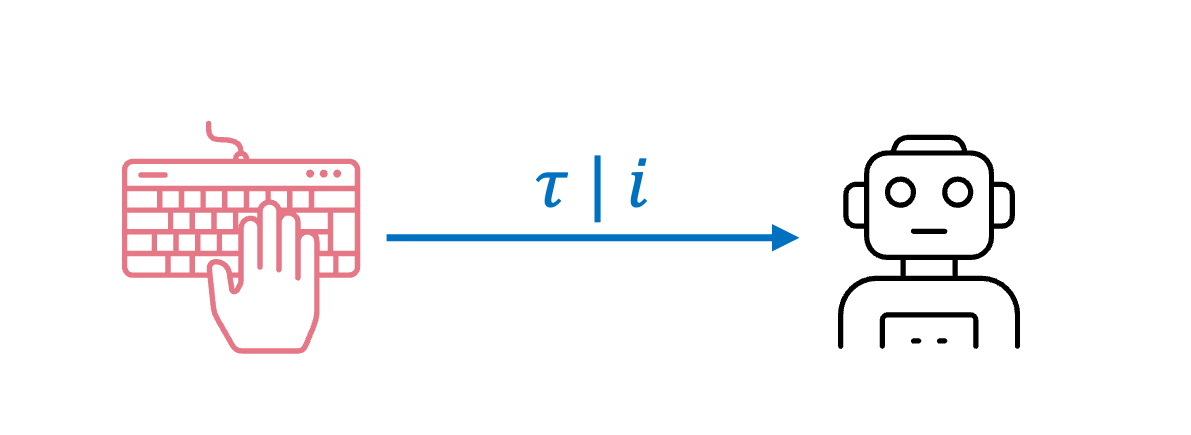
\includegraphics[width=0.7\linewidth]{figures/few_shot_1.png}
    \caption{Human-crafted.}
    \label{fig:few_shot_1}
  \end{subfigure}
  \hfill
  \begin{subfigure}{0.49\linewidth}
    \centering
    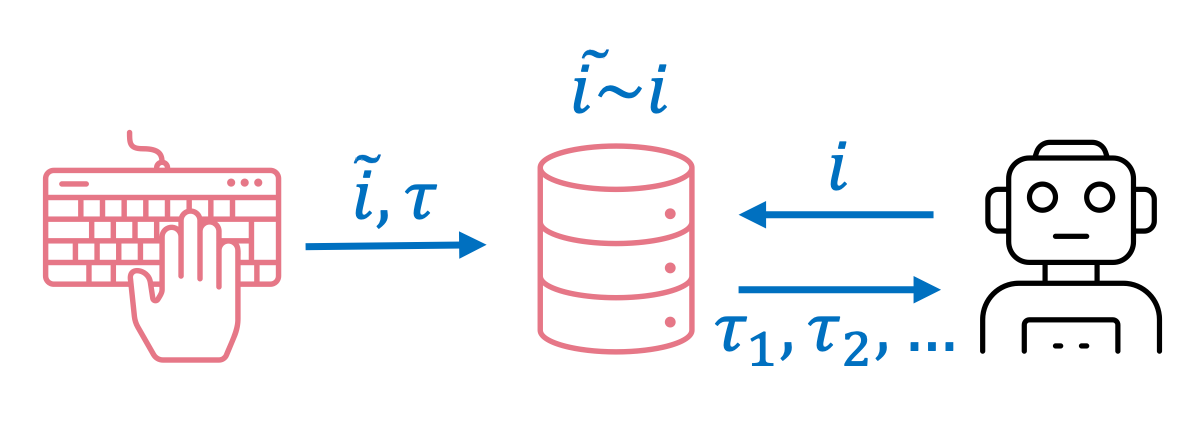
\includegraphics[width=0.7\linewidth]{figures/few_shot_2.png}
    \caption{Semantic search.}
    \label{fig:few_shot_2}
  \end{subfigure}
  \hfill
  \begin{subfigure}{0.49\linewidth}
  \centering
    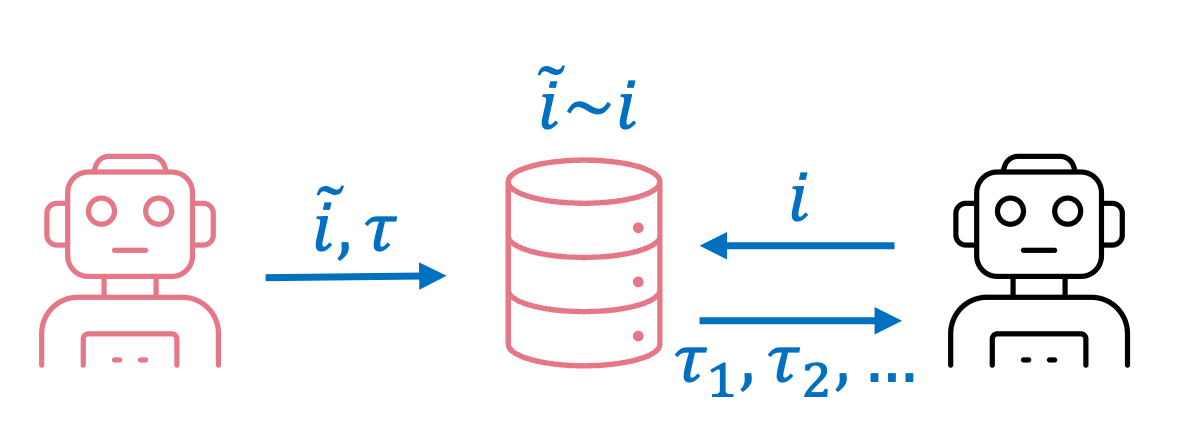
\includegraphics[width=0.7\linewidth]{figures/few_shot_3_n.png}
    \caption{Auxiliary model.}
    \label{fig:few_shot_3}
  \end{subfigure}
  \hfill
  \begin{subfigure}{0.49\linewidth}
  \centering
    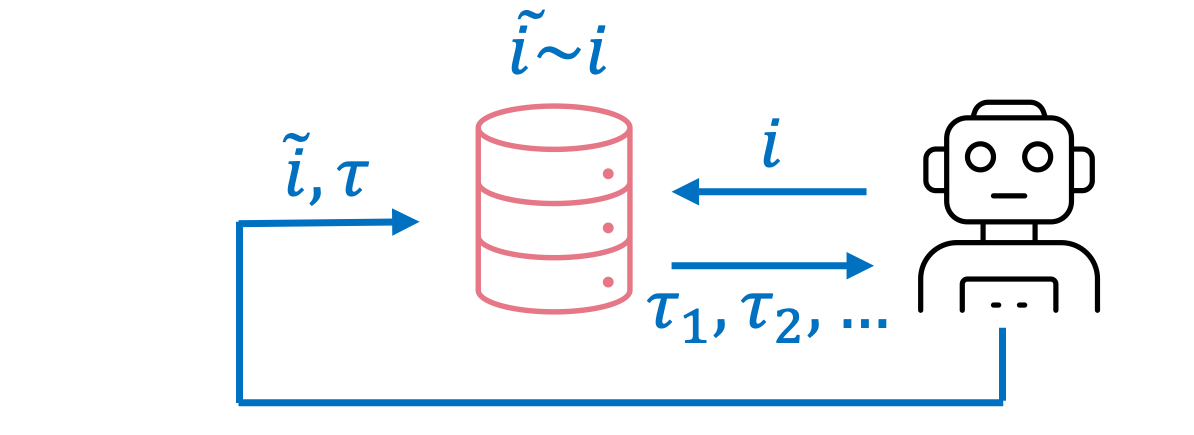
\includegraphics[width=0.7\linewidth]{figures/few_shot_4_n.png}
    \caption{Agent collected.}
    \label{fig:few_shot_4}
  \end{subfigure}
    \caption{The four most common few-shot learning strategies for ACUs.}
    \Description{
    This figure presents four common few-shot learning strategies for ACUs, each visualized through schematic subfigures involving a human (keyboard icon), an ACU (robot icon), and a demonstration store (cylinder icon). Arrows denote the direction and type of information flow, such as instructions $i$ and task demonstrations $\tau$, highlighting distinctions in data provenance and retrieval mechanisms. In (a) \emph{human-crafted}, the human directly provides demonstrations $\tau$ conditioned on $i$ to the agent. In (b) \emph{semantic search}, the human contributes $\tau$ and $i$ to a database, which the agent then queries bidirectionally to retrieve demonstrations. In (c) \emph{auxiliary model}, an auxiliary agent, rather than a human, populates the database with $\tau$ and $i$, while the main agent retrieves data as in (b), visually distinguishing the source of data via the origin of the arrows. In (d) \emph{agent collected}, the ACU both generates and retrieves demonstrations, forming a closed-loop interaction absent in other strategies and not explicitly detailed in the main text. These diagrams emphasize that although the textual descriptions may appear similar, the strategies differ fundamentally in terms of data origin and control flow.
}
    \label{fig:few_shot}
\end{figure}

\paragraph{Episodic Improvement through Planning} \label{sec:episodic_planning}

ACUs are goal-driven and often require planning to fulfill complex instructions $i$ \citep[Chapter~2.4]{russell_artificial_2022}. Most specialized agents perform implicit planning in their latent space, a process \citet{li_zero-shot_2023} called \emph{iterative planning}, where future states or action consequences are not explicitly constructed.

Agents based on foundation models typically generate explicit plans in text form. One common method is \emph{chain-of-thought} prompting \citep{liu_chain_2023}, which guides the model to produce intermediate reasoning steps before deciding on an action, improving the agent's performance \citepeg{rawles_android_2023, zhang_android_2024}. Another method involves decomposing an instruction into sequential sub-tasks, such as breaking down the task \texttt{Book an economy class flight from Hangzhou to Beijing} into steps like \texttt{Open the Alipay app} and \texttt{Input ``Hangzhou'' as the departure city} \citep{guan_intelligent_2023}. 

Plans can be refined iteratively.
For instance, after initial prompting, agents may either follow their initial plan rigidly \citepeg{kim_language_2023} or adapt it based on new observations \citepeg{sun_adaplanner_2023}.
Another refinement \citep{kim_language_2023} is done by prompting their foundation model to critique and refine its generated plans recursively. Although this can yield minor improvements, \citep{kambhampati_can_2024} argues that the benefits of self-critiquing may be limited.

These prompt-based planning strategies are considered informal planning, as they are based on the text output of foundation models, as opposed to internally simulating various action trajectories before deciding on one.
In contrast, formal planning can be implemented based on a search algorithm.
For instance, \citet{koh_tree_2024} simulate actions in a controlled environment and search through potential future states (observations) to better inform decision-making for the next action.
This approach shows significant performance gains, with task success rates improving by 50\% at a search depth of $5$. 
Building on this, \citet{chae_web_2024} fine-tune a model to predict the effects of actions on current observations, allowing for better decision-making without relying on an external simulator.
%Those ideas are similar to recent test-time compute techniques using agentic workflows \citep{snell2024scaling, singh2024enhancing}.



\subsubsection{Recommendations}
The landscape of learning strategies for ACUs is notably diverse.
Historically, RL and BC dominated as the primary paradigms. More recently, the emergence of foundation agents has shifted attention toward prompt-based learning. Despite this evolution, our analysis reveals that the field has yet to converge on a unified framework (see Appendix~\cref{fig:learning-strategy-dist}).

To enable a technology-agnostic characterization, we categorized learning paradigms into three sequential steps: pre-training, environment learning, and episodic improvement.
Our analysis reveals \textbf{a research gap in an effective and practical environment learning paradigm for foundation agents}:
Long-term memory approaches, while practical, often suffer from poor generalization. Storing raw trajectories is less beneficial than capturing underlying concepts, which remains highly challenging within this approach.
In contrast, reinforcement learning (RL) and behavioral cloning (BC) provide strong learning signals and enable concept abstraction, but they are highly resource-intensive, requiring either high-fidelity simulation environments or curated and labeled datasets for effective fine-tuning.

To address this bottleneck, we recommend research into the direction of introducing a \textbf{self-supervised fine-tuning stage between general pre-training and resource-intensive environment learning}. This intermediate stage would align general-purpose foundation models more closely to computer use contexts --- analogous to the role of RLHF in aligning LLMs with human preferences \citep{ziegler_fine_2020} or GRPO in improving reasoning \citep{shao2024deepseekmathpushinglimitsmathematical}. Such an alignment stage would equip models with domain-specific inductive biases, enabling faster and more robust adaptation during subsequent environment learning phases \citep{ouyang_training_2022}.

Our analysis also identifies planning as a major limitation in current ACU architectures. 
LLMs exhibit limited long-horizon planning capabilities \citep{valmeekam2023planning}, and the dynamics of the environment are often unknown, which hinders direct adaptation of symbolic approaches.
Thus, we argue that \textbf{planning in ACUs remains an open and pressing research challenge}. However, we identify two promising research directions for addressing this gap:
First, recent developments in reasoning-oriented LLMs, such as OpenAI o1, demonstrate promising capabilities in planning and long-horizon decision-making \citep{valmeekam2024llms, tan_towards_2024}. 
Adapting these capabilities for ACUs—and demonstrating robust planning performance in dynamic digital environments—is a critical next step.
Second, hybrid systems that combine symbolic planning with learned models of perception and action outcomes, such as those proposed by \citet{koh_tree_2024}, offer a compelling alternative. These methods draw from classical planning algorithms \citep[Chapter~11]{russell_artificial_2022} while leveraging neural components for generalization and flexibility.
% Forward state-space search could benefit from more agentic foundation models and approaches could adapt more sophisticated planning methods, such as using constraints \citep{porteous2001extraction,hoffmann2004ordered}.
Although these approaches extend beyond the ACU domain, we argue that ACUs provide an ideal testbed due to their complexity and fully digital nature. The integration of neuro-symbolic methods with agentic foundation models may pave the way for more sophisticated, adaptive, and general-purpose computer use agents.

\section{Computer Use Datasets}\label{sec:datasets}
In this section, we focus on important computer use datasets and do not cover datasets used for general pre-training of foundation models or those only partially relevant for computer use, such as question answering \citepeg{hudson2019gqa} and tool usage datasets \citepeg{patil2023gorilla}.
\Cref{tab:overview_datasets} provides an overview of all considered computer use datasets and their key properties.

To illustrate the evolution of these datasets, \Cref{fig:dataset-timeline} presents a timeline of their development across three major domains: Web, Android, and personal computers. The figure reflects a general trend toward increasing task complexity and realism over time, highlighting how research has shifted from simplified environments toward real-world applications and large-scale demonstrations.


\begin{figure}[t]
    \centering
    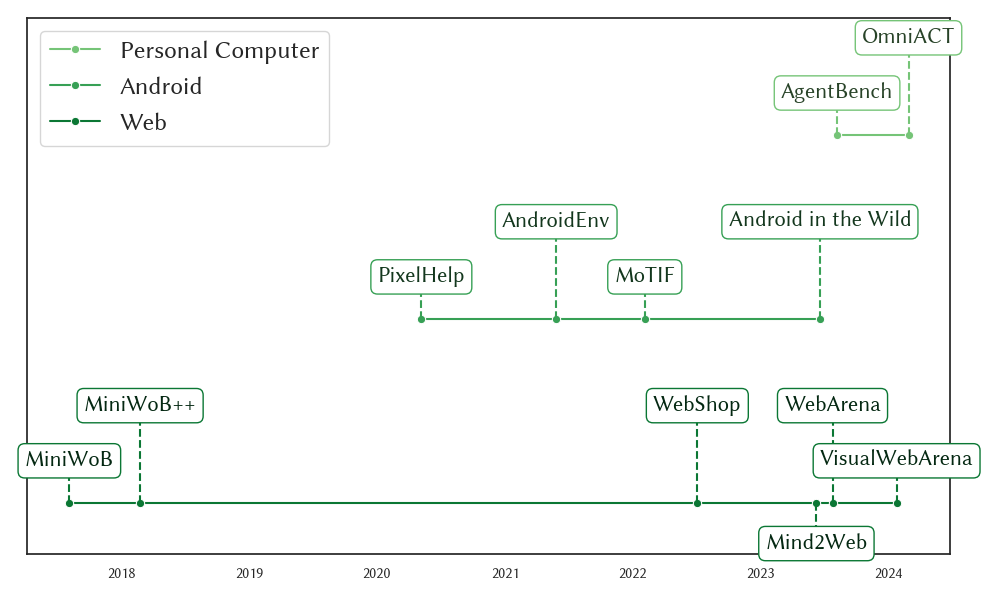
\includegraphics[width=0.7\linewidth]{figures/dataset_domain_timeline.png}
    \caption{Development of datasets across domains over time. In general, complexity increases over time. For the \emph{Web domain}: MiniWoB \citep{shi_world_2017} and MiniWoB++ \citep{liu_reinforcement_2018} contain $100$ tasks on a simplified UI. WebShop \citep{yao_webshop_2022} is a more realistic single webshop application focusing on realistic product diversity. Mind2Web \citep{deng_mind2web_2023} contains $2350$ demonstrations across $137$ actual websites. WebArena \citep{zhou_webarena_2024} is a controlled environment of $4$ realistic web applications. VisualWebArena \citep{koh_visualwebarena_2024} extends WebArena with $910$ more visual tasks and an additional application. For the \emph{Android domain}: PixelHelp \citep{li_mapping_2020} contains step-by-step instructions across $4$ applications. AndroidEnv \citep{toyama_androidenv_2021} provides a framework to define custom tasks in Android applications. MoTIF \citep{avidan_dataset_2022} contains $756$ demonstrations across 125 applications. Android in the Wild \citep{rawles_android_2023} provides over $700,000$ demonstrations across $357$ applications. For the \emph{personal computer domain}: AgentBench \citep{liu_agentbench_2023-1} is a benchmark framework that spans operating systems, databases, web, and gaming tasks, including existing benchmarks like WebShop or Mind2Web. OmniACT \citep{kapoor_omniact_2024} contains $9802$ tasks labeled with straight-line code actions spanning $57$ applications on Windows, MacOS, Linux, and the Web.}
    \Description{The figure shows the chronological order of dataset releases for Web, Android, and Personal Computer domains over the years 2017 to 2024. It reveals that the Web domain saw earlier development activity, starting in 2017, while large-scale Android and Personal Computer datasets began emerging around 2020 and 2023, respectively. The timeline also indicates a concentration of new datasets in 2023 and 2024 across all domains, suggesting recent intensified interest. Although dataset complexity is not visually encoded, the temporal arrangement highlights the evolving landscape of task diversity and domain coverage over time.}
    \label{fig:dataset-timeline}
\end{figure}

\subsection{Dataset Types}
% Computer use datasets must fulfill two properties:
% \begin{itemize}
%     \item \textbf{Teaching Signal:}  The dataset must provide a teaching signal, enabling the agent to receive feedback on its actions $a_t$ or trajectories $\tau$, which is essential for guiding the learning process.
%     \item \textbf{Isolated Execution:} Training is typically conducted offline, separate from the final deployment platform, to prevent the agent from executing tasks that could have real-world consequences, such as modifying production databases or booking flight tickets during the learning phase.
%\end{itemize}

ACUs leverage two types of computer use datasets:
%

\begin{description}
    \item[Controlled Environments:] 
    A controlled environment is a simulated setting, meaning an agent can act freely without consequences, as the simulation can always be reset.
    These environments support reinforcement learning, given they provide an additional reward signal  \citepeg{humphreys_data-driven_2022}.
    Furthermore, they can be utilized to collect long-term memories in a safe simulation phase \citepeg{wen_autodroid_2024} and to plan at inference time by simulating potential actions \citep{koh_tree_2024}.
    \item[Offline Dataset: ]
    An offline dataset is collected by instructing humans on a computer task while recording observations and executed actions.
    The agent only sees the recorded interaction during training, meaning it never acts in the underlying environment, making training safe from consequences.
    % Collecting human trajectories is more straightforward than creating a controlled environment.
    Offline datasets can be utilized for few-shot learning \citepeg{deng_mind2web_2023} or fine-tuning an agent \citepeg{rahman_v-zen_2024} in an uncontrolled environment like a productive website. Furthermore, an offline dataset of a controlled environment can be used for initial behavioral cloning to combat sparse rewards \citep{humphreys_data-driven_2022}.
\end{description}

Both dataset types have distinct characteristics. 
Controlled environments are costly to create because they involve engineering simulations that mimic real-world behaviors, but the agent can explore all aspects of the environment autonomously.
In contrast, offline datasets can be recorded in any environment, but are incomplete as not every possible interaction is captured.
Furthermore, offline datasets only show a single trajectory to achieve an instruction, but maybe multiple ones exist.


\subsection{Domains, Observation and Action Spaces}
By analyzing the domains of our $\numdatasets$ reviewed datasets, we find that the majority of existing datasets are from the Web domain \citepeg{zhou_webarena_2024} and Android domain \citepeg{rawles_android_2023}, while the personal computer domain \citepeg{hong_cogagent_2024} receives less attention (see Appendix~\cref{fig:dataset-domain-dist}).

The types of observations and actions available in these datasets vary depending on the domain and data collection method. For observations, some datasets provide only image screen representations \citepeg{rawles_android_2023}, some only textual screen representations \citepeg{pasupat_mapping_2018}, while others offer both \citepeg{chen_websrc_2021}. Regarding actions, some datasets focus solely on mouse/touch and keyboard actions \citepeg{kapoor_omniact_2024}, some provide direct UI actions \citepeg{chen_webvln_2024}, while others focus on task-tailored actions \citepeg{liu_agentbench_2023}.
\Cref{tab:overview_datasets} provides an overview.
% Executable code is generally absent from offline datasets, as it is not feasible to record all possible code snippets an agent could generate.
% 
In many cases, additional observation and action types can be generated through post-processing efforts. For instance, HTML representations can be rendered through a web browser to provide image-based screen representations.

\subsection{Dataset Complexity}
Several factors, including the size of the state, observation, and action spaces, and the diversity of the tasks, influence the complexity of a computer use dataset. 
%These factors vary significantly between controlled environments and offline datasets.

Controlled environments are often simplified and less diverse compared to offline datasets. 
For instance, in MiniWoB++ \citep{shi_world_2017}, all tasks are performed within a uniform, simplified website design with minimal graphical user interface (GUI) elements and clean HTML. 
Similarly, WebShop \citep{yao_webshop_2022} is limited to a single, simplified webshop application. 
While WebArena \citep{zhou_webarena_2024} offers more realistic web environments, it is limited to four tasks.

Offline datasets tend to feature more realistic observations, with the diversity depending on the variety of scenarios, such as how many websites were included.
For example, Mind2Web \citep{deng_mind2web_2023} records tasks from 137 websites across 31 categories, providing substantial diversity.
Similarly, Android in the Wild \citep{zhang_android_2024} records tasks spanning 357 Android apps or websites.
% Offline datasets collected within controlled environments inherit the simplicity of the controlled environment, limiting their complexity and diversity.

The complexity of tasks varies greatly across datasets. 
For example, MiniWoB++ \citep{shi_world_2017} includes 100 tasks with randomized text and an average of 3.6 actions per task, ranging from simple actions like clicking a button to more complex tasks like filling out a form to book a flight. 
WebShop \citep{yao_webshop_2022} offers 12,000 crowd-sourced instructions, all related to shopping, with an average of 11.3 actions per task. 
Mind2Web \citep{deng_mind2web_2023} provides 2,000 tasks averaging 7.3 actions, while WebArena \citep{zhou_webarena_2024} features 812 tasks, some requiring actions across applications, such as the task to create a Reddit account mirroring a GitLab profile.

Generally, the complexity of newer datasets increases as agents become more capable.
A straightforward way to do this is to make observations and tasks more diverse and challenging.
For example, WebArena \citep{zhou_webarena_2024} has a more realistic observation space than MiniWoB++ \citep{shi_world_2017}, and tasks require more actions to be achieved.
However, there are many other ways to increase complexity:
VisualWebArena \citep{koh_visualwebarena_2024} adds images as part of the instruction, such as asking an agent to create a post selling a product shown in an image.
%\texttt{Help me make a post selling this item and navigate to it. Price it \$10 cheaper than the most similar item on the site}. 
AgentStudio \citep{zheng_agentstudio_2024} provides video-based observations, requiring agents to process dynamic, time-dependent information. 
MT-Mind2Web \citep{deng_multi-turn_2024} extends Mind2Web by introducing multi-turn tasks, where users give sequential instructions to the agent, requiring a more nuanced agent behavior.
MoTIF \citep{avidan_dataset_2022} introduces infeasible instructions in its offline dataset, challenging agents to recognize unachievable tasks.

\subsection{Recommendations}
\begin{comment}
A key limitation of current datasets lies in their insufficient task complexity, with most tasks within existing datasets involving a limited number of actions (averaging fewer than 10).
While increasing the number of actions can contribute to complexity, a more significant factor lies in the nature of these actions.
Actions can causally depend on previous actions, increasing task complexity.
For example, a meeting suggestion based on availability can only occur \emph{after} looking up available time slots.
In contrast, some actions can be performed in any order, such as filling out form fields, which typically indicates their independence from one another.
As such, we recommend that \textbf{future ACU datasets to increase the task complexity by requiring more actions, specifically causally dependent actions}.
\end{comment}


A key limitation of current datasets lies in their insufficient trajectory complexity. They have limited structural and causal dependencies between actions in a task sequence. Complex tasks often require agents to execute actions in a specific causal order, where later actions depend on the outcomes of earlier ones. For instance, proposing a meeting time requires first retrieving the user's availability. In contrast, filling form fields can often be performed in any sequence. We recommend that \textbf{future ACU datasets increase trajectory complexity} by designing tasks that require longer, causally dependent action sequences.

Although trajectory complexity is crucial, observation, action, and task diversity should not be neglected, as broader observation and action types (e.g., dealing with various UI components) and more diverse tasks within and across applications are essential for accurately reflecting real-world usage and improving the generality of agents.


\section{Agent Evaluation}\label{sec:evaluation_agent}
\begin{figure}
    \centering
    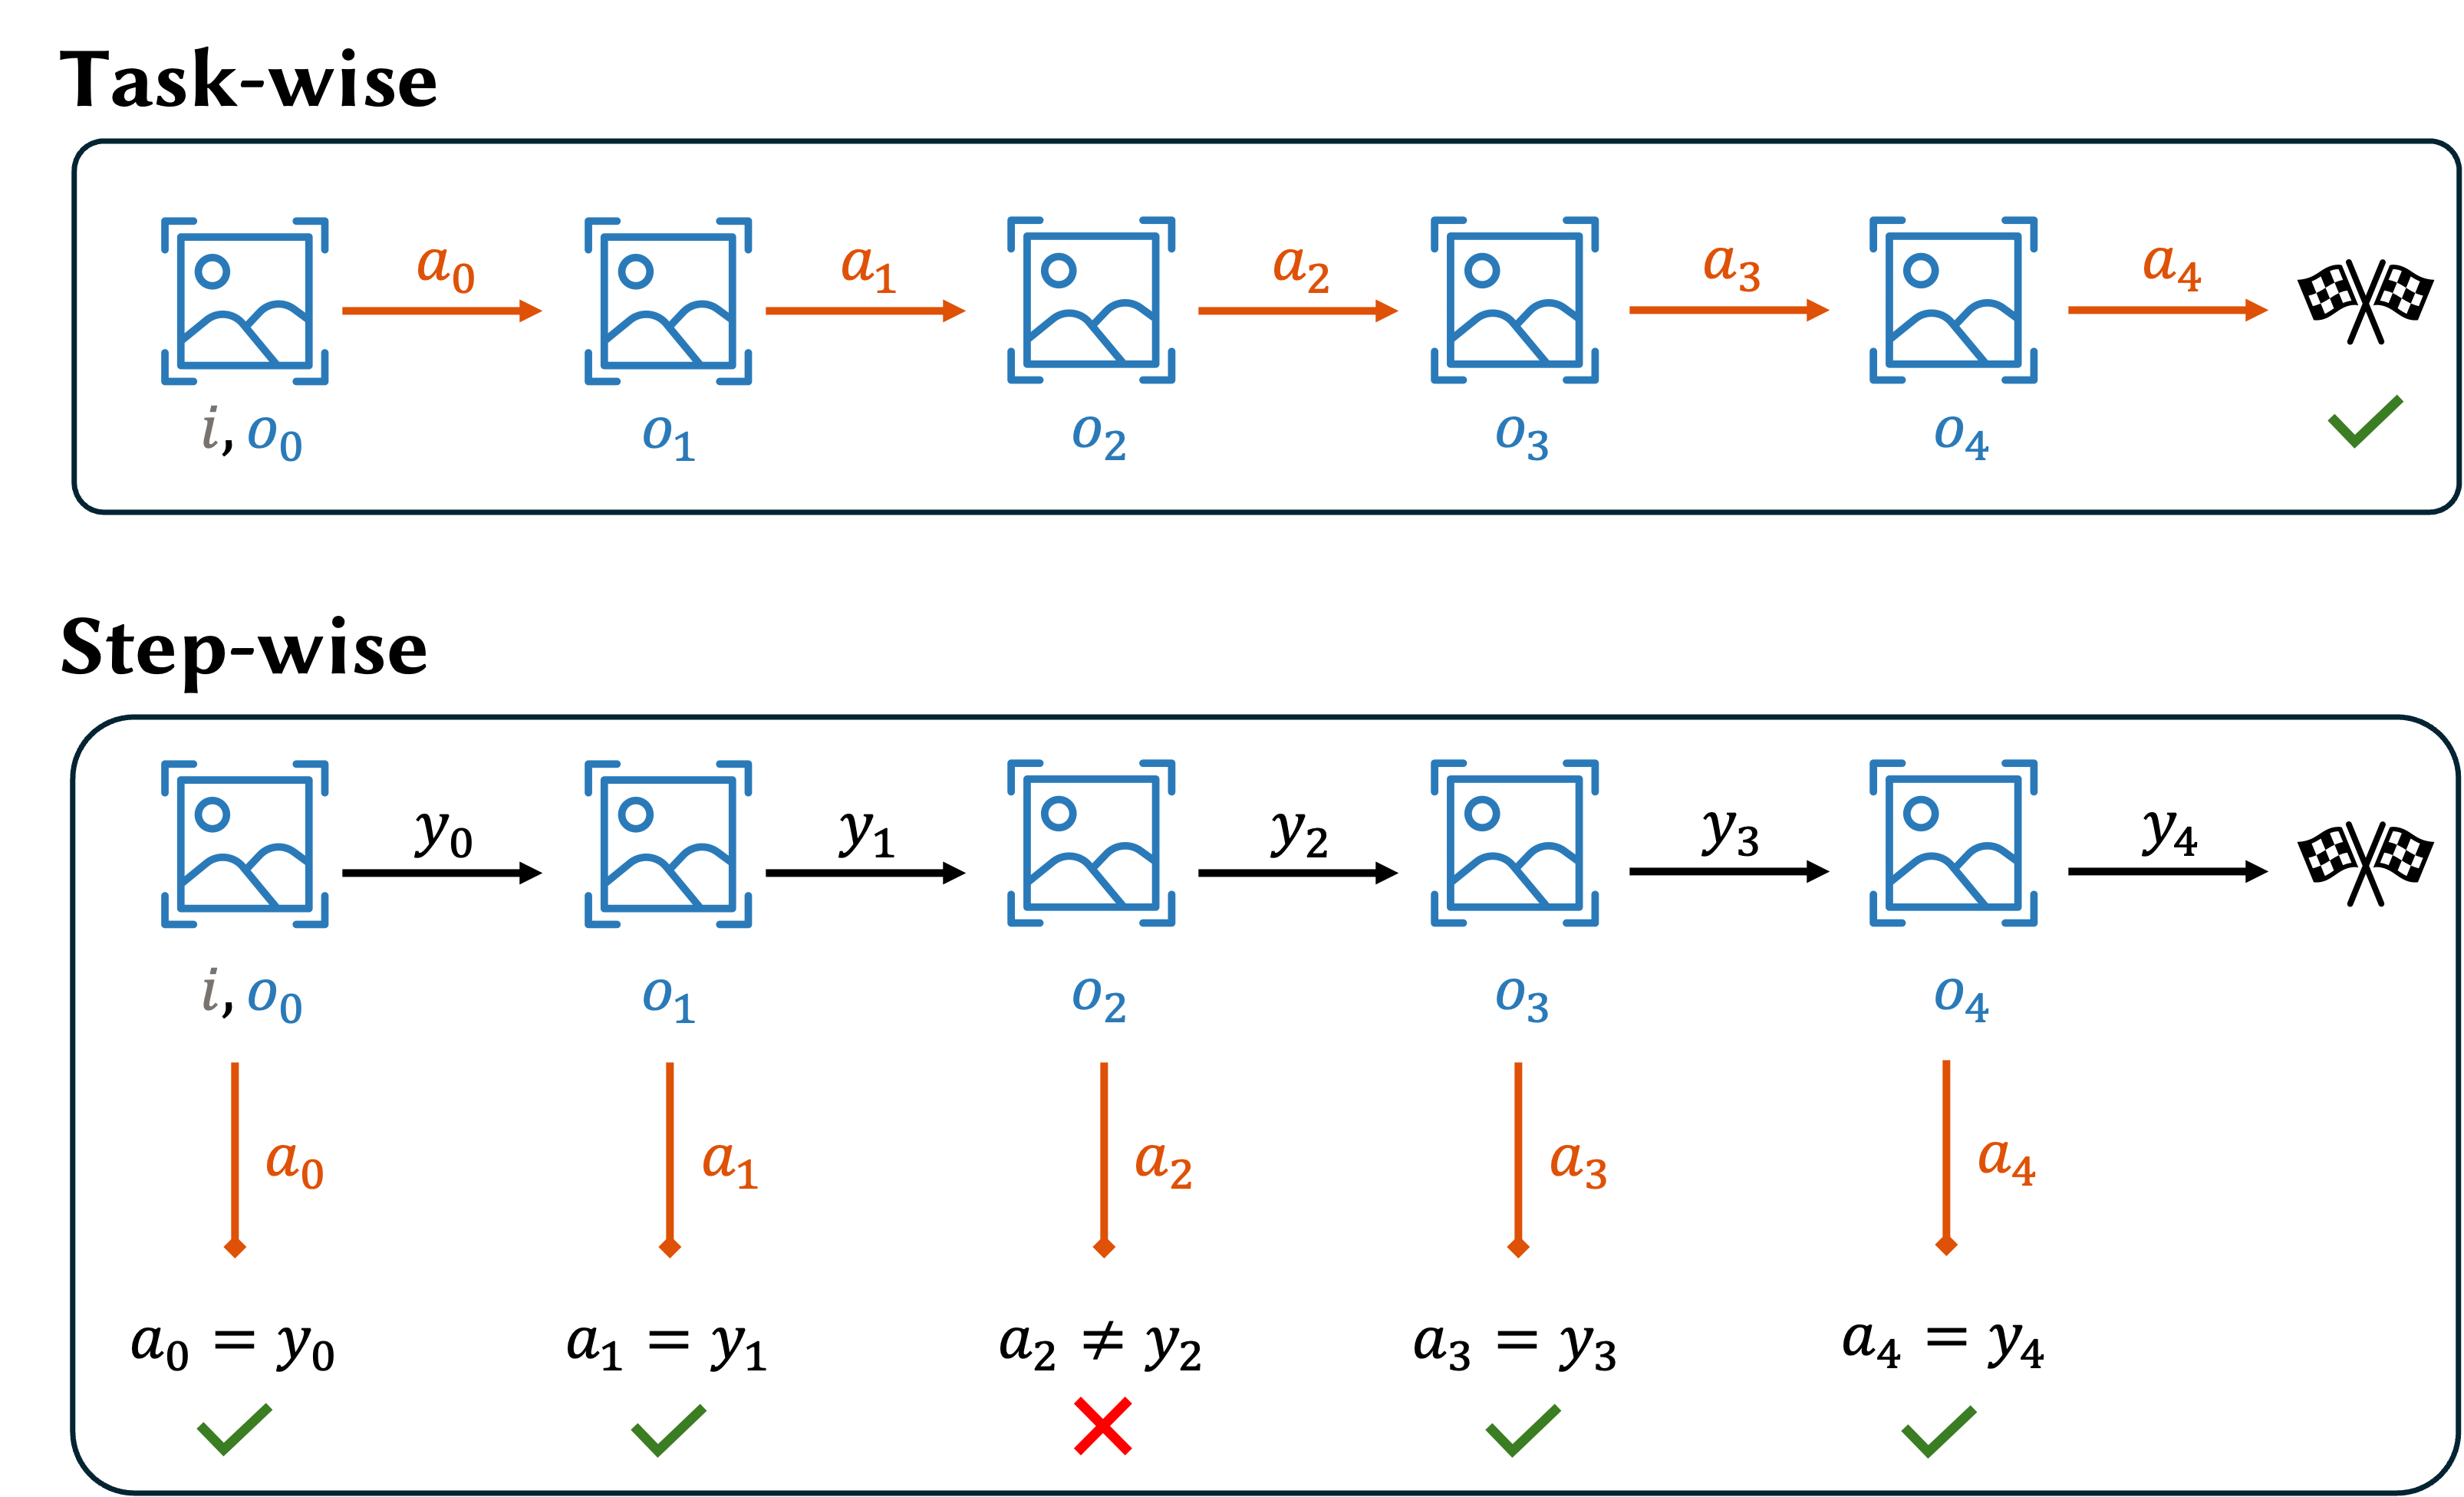
\includegraphics[width=0.6\linewidth]{figures/evaluation_types.png}
    \caption{Task-level metrics measure performance across individual tasks (instructions). Step-level metrics measure performance across individual steps (actions).}
    \Description{The figure contrasts two evaluation approaches. In both cases, a sequence of four generic observations and a single instruction is shown. In the task-wise evaluation (upper part), transitions between observations result from the model's predicted actions, and evaluation is performed only at the final observation. In the step-wise evaluation (lower part), transitions follow ground-truth actions, and the performance metric is computed after each individual prediction. A green checkmark visually indicates when evaluation occurs. Specific content of observations and instructions is not depicted, as they serve only to illustrate the evaluation paradigms.}
    \label{fig:evaluation_types}
\end{figure}

Various evaluation metrics are used in the current literature. 
We identify three groups of evaluation metrics (see also \cref{fig:evaluation_types}): \emph{Task-level metrics}, \emph{step-level metrics}, and \emph{other metrics}.  

\subsection{Task-Level Metrics}
Task-level metrics focus on the overall effectiveness of an agent in achieving an instruction $i$.
\emph{Task success rate} is the most common task-level metric, which measures the overall success rate of completing an entire task \citep{deng_mind2web_2023,zhang_android_2024}.
For controlled environments, the environment state indicates successful task completion. 
For offline datasets, an agent predicting the full trajectory correctly counts as successful task completion, termed \emph{offline task success rate} (also called complete match \citepeg{li_mapping_2020}).

The offline task success rate underestimates the actual task success rate, as it only considers a single recorded trajectory, whereas alternative valid trajectories may exist. Consequently, it serves as a \emph{lower bound} on the true task success rate.
To obtain a more accurate estimate, the \emph{online task success rate} can be used. To measure online task success rate, the agent must be deployed in its original environment, typically the live websites from which the offline dataset was collected. 
Human evaluators then determine whether the agent successfully completes the task \citep{zheng_gpt-4vision_2024, song_restgpt_2023, li_sugilite_2017}. Notably, \citet{zheng_gpt-4vision_2024} report that their agent's success rate increased from 12\% to 36\% when evaluated online, highlighting the limitations of relying solely on offline trajectories.
However, the reproducibility of the online task success rate poses a challenge, due to potential changes in the online environment and the potential for error in human evaluation \citep{reason1990human}.

Other, less common task-level metrics exist, often providing a more nuanced assessment of the agent's capabilities.
\emph{Task progress} measures the average task completion progress, meaning how far the agent, on average, is to complete a task \citepeg{sodhi_heap_2023, zhang_android_2024}.
\emph{Average reward} captures the average reward obtained across episodes within a controlled environment \citepeg{jia_dom-q-net_2019}. 
% It is worth noting that while these metrics are useful for comparing agents during development, they are not suitable for comparing agents across different environments, as they depend on the environment.

\subsection{Step-Level Metrics}

Step-level metrics focus on the overall effectiveness of an agent in predicting actions (steps) across tasks.
\emph{Step success rate} is the most common step-level metric, which assesses the accuracy of action prediction \citepeg{deng_mind2web_2023}.
In the literature, step success rate is also called \emph{partial match} \citepeg{li_mapping_2020} or \emph{action accuracy} \citepeg{wen_autodroid_2024}.

Each step (action) is part of a trajectory (a sequence of multiple actions), which in turn represents a single task in the dataset (comprising multiple tasks). Consequently, step-level metrics must define how to average step scores both within their trajectory and across tasks, similar to other fields like multi-class classification, where metrics are averaged within classes and across samples \citep{grandini2020metrics}.
Two natural approaches for averaging exist:

\begin{description}
    \item[Macro averaging:] 
        Step scores are averaged first within their respective trajectory and then across tasks. As a result, each step score is weighted by the inverse of its corresponding trajectory's length.
    \item[Micro averaging:] 
        Step scores are averaged across all steps (of all trajectories). This assigns equal weight to each step score regardless of trajectory length.
\end{description}

For computer use, \emph{macro averaging} seems to be the prevailing approach, established by Mind2Web \citep{deng_mind2web_2023} and adopted by subsequent work \citepeg{zheng_synapse_2024}.

Other less common step-level metrics include the \emph{action F1} score \citepeg{li_mug_2024}, \emph{action recall} \citepeg{li_glider_2021}, or measuring only if parts of the action are correct, like the \emph{element accuracy} for direct UI access actions \citepeg{deng_mind2web_2023}.
Finally, all step-level metrics only exist for offline datasets, as controlled environments' rewards do not indicate the correctness of individual actions.


\subsection{Other Metrics}

Other metrics in the literature measure performance indicators other than an agent's capabilities.
\citet{song_restgpt_2023} evaluate agent \emph{efficiency} by measuring the number of API calls required to execute an instruction successfully, emphasizing minimal resource usage during task execution.
\citet{zhang_ufo_2024} incorporate a safeguard mechanism to seek user confirmation before executing critical actions (e.g., delete) to build a safer and more trustworthy agent. The \emph{safeguard rate} measures how accurately the agent identifies sensitive actions and requests user confirmation. 

\subsection{Recommendations}
A standardized evaluation protocol is currently absent in the ACU literature. A key challenge lies in the prevalent use of custom datasets or modified benchmarks to highlight specific strengths \citepeg{wang_mobile-agent_2024,wen_autodroid_2024}, which limits comparability across studies.
For instance, in the MiniWoB++ benchmark \citep{shi_world_2017,liu_reinforcement_2018}, different studies have adopted varying subsets of tasks, complicating cross-study comparisons. \citet{humphreys_data-driven_2022} evaluated agents on all 104\footnote{MiniWoB++ currently includes 100 tasks, excluding four that violate the static assumption.} tasks, while \citet{zheng_synapse_2024} used 64 tasks and \citet{kim_language_2023} selected 55. 
Despite these differences between ACU evaluations, average task performance is compared directly, undermining fair assessment. 
For example, \citet[Figure 3]{zheng_synapse_2024} and \citet[Figure 4 (b)]{kim_language_2023} compared their average task performance on a subset of tasks with an ACU evaluated on the full benchmark.

Moreover, no consensus exists on how to measure agent performance.
Among the available performance metrics, the task success rate best reflects practical agent capabilities, as it evaluates whether an agent completes a task in its entirety.
In contrast, step-level metrics measure the performance across individual steps and can be misleading when assessing actual agent competence, as a single error in a lengthy action trajectory may have substantial real-world consequences but only a minor influence on step-level metrics.
Accordingly, we recommend that for evaluating performance, \textbf{ACU publications should report the task success rate as the primary metric on established and complete benchmarks}.

While task success rate can be reliably measured in controlled environments, it is challenging for offline datasets. 
Reporting the offline task success rate provides only a lower bound and might underestimate agent performance; reporting the online task success rate is labor-intensive and suffers from limited reproducibility due to evolving online environment conditions and different evaluation procedures.
In such offline dataset settings, the step success rate can serve as a reproducible proxy that must be interpreted with caution:
First, it is a conservative estimate of actual step correctness, as alternative valid actions are often not captured in the dataset and penalized as errors.
Second, higher step-level accuracy does not necessarily translate to higher task-level performance.

For evaluations on offline dataset benchmarks, we recommend reporting both the step success rate as a reproducible proxy metric and, where possible, the online task success rate as a measure of actual agent performance. To improve comprehensibility and traceability, the online evaluation protocol should be thoroughly documented, including details such as the date of the evaluation and any strategies used to mitigate human error \citep{reason1990human}.

Finally, ACUs must be capable of predicting a deliberate \texttt{stop} action to signal task completion. This capability is critical both for practical deployment and for correctly identifying when a task has been completed \citepeg{wang_mobile-agent_2024}. We therefore recommend requiring a \texttt{stop} action in ACU evaluations whenever feasible and suggest that future benchmarks enforce this requirement. For example, controlled environments could reward agents only after they reach the goal state and explicitly issue the stop action.

\input{imported_papers/ACU_JAIR/sections/08_challenges}


% ─────────────────────────────────────────────────────────────────────────────
\section{Chapter Summary}
\label{sec:acu_chapter_summary}
% ─────────────────────────────────────────────────────────────────────────────

This chapter has presented a comprehensive survey and taxonomy of agents for
computer use, covering 87 original research papers and 33 benchmark datasets
spanning the period 2018 to 2024. The three-perspective taxonomy — domain,
interaction, and agent — provides a technology-agnostic organisational
framework that bridges the previously fragmented literatures on
reinforcement-learning-based agents and foundation-model-based agents, enabling
systematic comparison across architectures and training paradigms.

Three structural trends characterise the current state of the field. The field
is transitioning from specialised, task-specific agents toward foundation-model-based
agents that leverage pre-trained vision-language models for open-ended reasoning.
The dominant observation modality is shifting from structured text
representations, such as HTML and accessibility trees, toward raw screenshots,
reflecting both the fragility of text-based observations and the improving
visual capabilities of foundation models. Behaviour cloning from human
demonstrations has emerged as the dominant learning paradigm among agents that
do learn from experience, though its data requirements and limited adaptability
represent significant practical constraints.

The primary finding of the survey, and its central contribution to the
thesis argument, is the identification of six persistent research gaps that
recur across the surveyed systems independently of their specific architecture,
training procedure, or platform:

\begin{enumerate}
    \item \textbf{Insufficient generalisation.} ACU systems fail reliably when
    interface layouts, task formulations, or environmental conditions differ
    from those encountered during training. The failure pattern is not one of
    missing data but of missing representational structure: systems cannot
    recombine familiar components in novel configurations.

    \item \textbf{Inefficient learning.} Current systems require large volumes
    of demonstration data and do not transfer learned behaviour effectively to
    related tasks. Sample inefficiency is systematic, not incidental, and
    reflects the absence of structural priors that would make infrequently
    encountered situations tractable.

    \item \textbf{Limited planning.} Reliable execution of long-horizon tasks
    requires maintaining a coherent model of task state and anticipating the
    effects of future actions. Current systems fail along both dimensions, either
    drifting from the goal over long autoregressive sequences or relying on world
    models whose predictions diverge exponentially with rollout length.

    \item \textbf{Low task complexity in benchmarks.} Widely used benchmarks
    evaluate agents on tasks that are systematically simpler than real-world
    computer use in sequence length, environmental variability, and success
    criterion complexity. Strong benchmark performance does not reliably predict
    strong deployment performance.

    \item \textbf{Non-standardised evaluation.} The absence of shared evaluation
    protocols makes direct comparison between systems unreliable. Reported
    success rates are not comparable across works, inflating the apparent
    progress of the field.

    \item \textbf{Disconnect between research and practical conditions.} ACU
    systems are developed and evaluated in static, deterministic, idealised
    environments. Real-world deployment introduces dynamic interfaces,
    non-stationarity from software updates, privacy constraints, and the need
    for conditional rather than full autonomy — properties that are absent from
    virtually all existing research settings.
\end{enumerate}

These six gaps are not independent failures of individual systems. They are
manifestations of a common pattern: current AI systems exhibit high competence
within the statistical regime of their training distribution and systematic
brittleness outside it. The specificity of this pattern demands a specific
explanation.

The standard response in the field is to attribute the gaps to insufficient
scale or to benchmark limitations, and to predict that they will close as
models and datasets grow. The evidence presented in this chapter does not
support this prediction. The generalisation and planning failures persist in
the largest and most capable foundation models currently evaluated on ACU
benchmarks. The benchmark complexity gap is not narrowing: as benchmarks
become more realistic, the gap between evaluated performance and the minimum
required for practical deployment remains substantial. And the disconnect
between research conditions and deployment conditions is structural — it
reflects assumptions baked into experimental design, not a shortfall in
model capacity that additional compute can correct.

Part~\ref{part:diagnosis} takes up the question of what these failures do
indicate. Chapter~\ref{chap:selfattention} establishes, at the level of
mathematical proof, that the representational geometry produced by
gradient-based training on standard objectives is determined by the structure
of the training signal rather than by the causal structure of the world.
The six gaps identified here are, under this account, predictable consequences
of a learning paradigm that encodes statistical correlations rather than
invariant structure. This reframing has direct implications for what kinds of
interventions can address the gaps — a question taken up in Parts~\ref{part:constraints}
and~\ref{part:paradigm}.

\chapter{Limitations of Foundation Models}
\margintoc
\input{sections/3-2_llm_benchmark}

\chapter{Compositional Generalization Remains Unsolved}
\margintoc
\input{sections/3-3_cogitao}

%----------------------------------------------------------------------------------------
%	PART III: Root Causes
%----------------------------------------------------------------------------------------

\pagelayout{wide}
\addpart{Root Causes — What Backpropagation Actually Learns}
\pagelayout{margin}

\chapter{The Mathematical Structure of Self-Attention — Symmetry, Directionality, and Statistical Correlation}
\margintoc
\input{sections/4-1_attention}


%----------------------------------------------------------------------------------------
%   PART IV: Mitigating the Limitations — Hard Constraints and Inductive Biases
%----------------------------------------------------------------------------------------

\pagelayout{wide}
\addpart{Mitigating the Limitations — Hard Constraints and Inductive Biases}
\pagelayout{margin}

\chapter{Koopman-JEPA — Enforcing Linear Dynamics for Stable World Models}
\margintoc
\input{sections/5-1_koopman_jepa}

\chapter{Input-Space Constraints via Domain Knowledge: Hounsfield Units for CT Segmentation}
\margintoc
\input{sections/5-2_hounsfield}

\chapter{Inference-Time Grounding via Hybrid Retrieval}
\margintoc
\input{sections/5-3_retrieval}


%----------------------------------------------------------------------------------------
%   PART V: PARADIGM CHANGE
%----------------------------------------------------------------------------------------

\pagelayout{wide}
\addpart{A Change of Paradigm — Neuro-Inspired Architectures}
\pagelayout{margin}

\chapter{The Cooperative Network Architecture — Structured Assemblies as an Alternative to Distributed Representations}
\margintoc
\input{sections/6-1_cna}

%----------------------------------------------------------------------------------------
%   PART VI: DISCUSSION AND CONCLUSION
%----------------------------------------------------------------------------------------

\pagelayout{wide}
\addpart{Synthesis and Conclusion}
\pagelayout{margin}

\pagelayout{wide}
\addpart{Synthesis}
\pagelayout{margin}

\chapter{Discussion}
\margintoc
\input{sections/7-1_discussion}

\chapter{Conclusion}
\margintoc
\input{sections/7-2_conclusion}

\appendix % From here onwards, chapters are numbered with letters, as is the appendix convention

\pagelayout{wide} % No margins
\addpart{Appendix}
\pagelayout{margin} % Restore margins

\chapter{Additional Material}

Additional material goes here.


%----------------------------------------------------------------------------------------

\backmatter % Denotes the end of the main document content
\setchapterstyle{plain} % Output plain chapters from this point onwards

%----------------------------------------------------------------------------------------
%	BIBLIOGRAPHY
%----------------------------------------------------------------------------------------

\defbibnote{bibnote}{Here are the references in citation order.\par\bigskip} % Prepend this text to the bibliography
\printbibliography[heading=bibintoc, title=Bibliography, prenote=bibnote] % Add the bibliography heading to the ToC, set the title of the bibliography and output the bibliography note

%----------------------------------------------------------------------------------------
%	INDEX
%----------------------------------------------------------------------------------------

\printindex % Output the index

\end{document}
